\documentclass[12pt,a4paper,titlepage]{book}

\usepackage[utf8]{inputenc}
\usepackage[french]{babel}
\usepackage[T1]{fontenc}
\usepackage{amsmath}
\usepackage{amsfonts}
\usepackage{amssymb}
\usepackage{graphicx}
\usepackage{subcaption}
\usepackage[babel=true]{csquotes}
\usepackage[left=2cm,right=2cm,top=2cm,bottom=2cm]{geometry}
\usepackage{braket}
\usepackage{pdfpages}

\title{NOTES DU COURS DE MÉCANIQUE QUANTIQUE 2}
\author{Baptiste CALVEZ}
\date{L3 Physique}

\begin{document}
\maketitle
\pagenumbering{gobble}
\newpage
\null
\newpage
\begin{center}
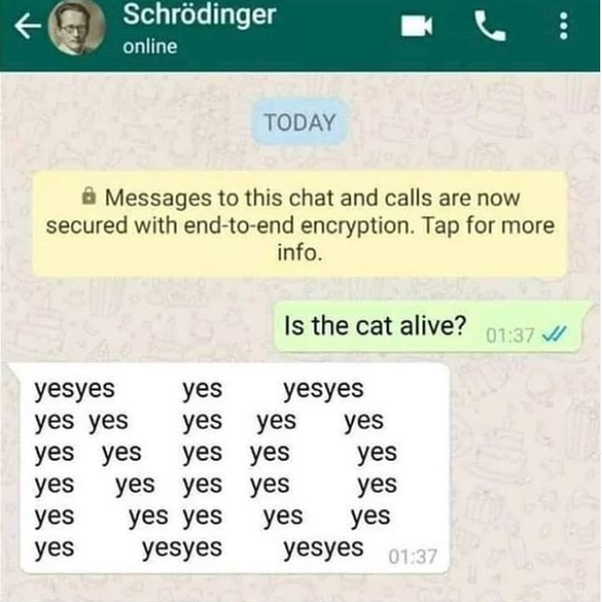
\includegraphics[scale=0.5]{memereddit.png}

\includegraphics[scale=0.2]{memereddit2.png}
\end{center}

\textit{en haut : Reddit : r/physicsmemes, Schrödinger's alive!! par u/Helpful\_{}Option\_{}7678}\\

\textit{au dessus : Reddit : r/physicsjokes, Double slit guilt par u/Egren}
\newpage
\null
\newpage
\pagenumbering{arabic}
\tableofcontents
\newpage
\chapter*{PRÉFACE}

Ce document est une mise en forme de mes notes de cours, c'est à dire que toutes les abréviations que j'ai utilisé sont remplacées par ce qu'elles abrégeaient. Comme il s'agit de mes notes de cours, des erreurs peuvent s'y être glissée. J'ai également complété mes notes de cours avec des recherches personnelles, qui seront insérées dans des encadrés.\\

Étant donné la certaines longueur du cours, je propose en fin de ce document un \enquote{essentiel du cours}, qui consiste principalement à vous donner les formules et phrases importantes du cours avec le numéro de la page pour compléter et retrouver rapidement le passage en question.\\

Plusieurs parties du cours, notamment des démonstrations, eurent lieu en travaux dirigés. De même, comme dit plus tard, ce cours contient de nombreuses références au \enquote{Cohen}. Il s'agit du livre de Claude Cohen-Tannoudji \enquote{Mécanique Quantique}.\\

Aussi, il y a un trou dans le premier chapitre du cours, à l'écriture de ce document.\\

Ce document a été rédigé en {\LaTeX} sur TeXmaker, sous GNU/Linux Ubuntu 20.04 LTS.\\

\newpage
\chapter*{CONSTANTES \& ABRÉVIATIONS}

\begin{tabular}{|p{15cm}|}
\hline
$\blacksquare$ Abréviations :\\
\hline
\enquote{cst} : constante.\\
\hline
\end{tabular}\\

\begin{tabular}{|p{15cm}|}
\hline
$\blacksquare$ Constantes :\\
\hline
e : nombre d'Euler, où $e \approx 2.781~218~282~459~045~\ldots$.\\
$\pi$ : Pi, nombre irrationnel, parfois appelé constante d'Archimède. $\pi \approx 3,141~592~653~589~793~\ldots$.\\
$h$ : constante de Planck, elle a pour valeur (fixé par convention le 20 mai 2019) 6,626 070 15 $\times 10^{-34}$ J.s. Son unité est le Joule seconde (J.s), et est de dimension $[h] = M.L^2.T^{-1}$. À noter qu'elle est à la base de la définition du kilogramme.\\
$\hbar$ : constante de Planck réduite, aussi dite constante de Dirac. Elle est égale à la constante de Planck divisé par $2\pi$. Elle est lié au fait qu'en mécanique quantique, il est plus \enquote{naturel} de parler en fréquence angulaire que de la fréquence, c'est à dire, s'exprimer en radians par seconde plutôt qu'en hertz. Ce qui a conduit à coupler la constante de Planck avec le facteur $2\pi$. Son unité est $kg.m^2.s^{-1}.rad^{-1}$ et sa dimension est $[\hbar] = M.L^2.T^{-1}.[rad]^{-1}$.\\
\hline
\end{tabular}\\

\begin{tabular}{|p{15cm}|}
\hline
$\blacksquare$ Symboles mathématiques :\\
\hline
$\mathcal{C}$ : Ensemble des nombres complexes ($z = a \pm ib$).\\
cos : fonction cosinus.\\
d, dt, dx : dérivée, dérivée selon t (généralement le temps), dérivée selon x.\\
$\partial$ : dérivée partielle.\\
$\in$ : appartient à.\\
exp(x) : fonction exponentielle. S'écrit également $e^x$ où e est le nombre d'Euler.\\
$\perp$ : est perpendiculaire à.\\
$i$ : nombre imaginaire ($i^2 = -1$).\\
$\sum$ : somme de (aussi dit sigma de).\\
sin : fonction sinus.\\
$\Re$ : partie réelle d'un nombre.\\
$\Im$ : partie imaginaire d'un nombre.\\
$\propto$ : est proportionnel à.\\
\hline
\end{tabular}\\

\newpage
\chapter*{INTRODUCTION AU COURS}

Comme dit dans la préface, ce document est une retranscription de mes notes du cours de Mécanique Quantique 2, dont les cours magistraux furent assurés par Arfa MONDHER. Ce cours fait suite au cours Mécanique Quantique de Gilles VIEN NGUYEN, qui eu lieu en licence 2 Physique. Ce cours, ou équivalent dans d'autres universités, est un prérequis à ce présent cours. Ces deux cours ont été dispensé à l'Université de Bretagne Occidentale à l'UFR de Sciences $\&$ Techniques à BREST.\\

Avant de parler du contenu du présent, faisons un résumé du cours précédent. Dans le dernier cours, nous avons vu les origines de la mécanique quantique, le comportement ondulatoire classique, allant de la définition de la longueur d'onde à la cohérence, aussi appelé \enquote{train d'ondes} en passant par la superposition, les interférences...\\

Ensuite, le cours précédent est revenu sur l'ensemble des rayonnements électromagnétique situés entre 400 nm et 700 nm, dit visibles, plus simplement : la lumière. Il fut rappelé l'histoire de l'étude de la lumière depuis le XVII$^e$ siècle avec les travaux de Kepler (propagation rectiligne de la lumière) de Descartes (loi de la réfraction) et de Newton. Rapidement, il fut démontré que la lumière possède un comportement de particule mais également un comportement ondulatoire (dualité onde - corpuscule ; mise en évidence par l'expérience des fentes de Young). L'un des points importants dans l'histoire de la mécanique quantique, le rayonnement du corps noir permit d'introduire, dans le cours, des constantes importantes tel que la constante de Planck ($h = 6.6 \times 10^{-34} Js$).\\

Max Planck fut celui qui introduit la notion de \enquote{quanta} d'énergie (d'où la mécanique quantique tire son nom). Le cours poursuit sur les nombreux travaux ayant lieu entre la toute fin du XIX$^e$ siècle et au début du XX$^e$ siècle sur l'atome (avec Thomson, Rutherford et Bohr principalement). Nous revenons ensuite sur la dualité onde-corpuscule où l'on aborde en détail l'expérience des fentes de Young, la notion du paquet d'onde et l'interprétation des inégalités de Heisenberg.\\

Après que les fondements de la mécanique quantique furent abordés, le cours se pencha ensuite sur la notion très importante en mécanique quantique qu'est la probabilité, par la loi de Malus notamment. Le cours de \enquote{Mécanique Quantique} dispensé en licence 2 termine sur des points qui seront vu plus loin dans les premiers chapitres ce présent cours, tel que la notation de Dirac (les bras et les kets), la notion d'hermitien / hermitique, les adjoints, la mesure de grandeurs physiques et l'équation de Schrödinger.\\

Le cours de \enquote{Mécanique Quantique 2} abordera, quand à lui, les aspects suivants de la discipline : l'espace des fonctions d'ondes, où nous profiterons pour revenir sur la notation de Dirac, les opérateurs hermitiques et les adjoints, pour finir sur les ensembles d'observables qui commutent. Nous verrons ensuite les six postulats de la mécanique quantiques, leurs interprétations physiques, mais aussi nous résoudrons l'équation de Schrödinger. Nous enchaînerons avec le magnétisme atomique où nous mettrons en évidence le spin.\\

Puis viendra une pause pour introduire de nouveaux concepts mathématiques, tel que les ondes planes, les transformées de Fourier, la généralisation aux fonctions à trois dimensions et le produit tensoriel. Nous poursuivront en abordant le potentiel à une dimensions constant par morceau, où nous verrons la continuité de la fonction d'onde, le théorème de Wronshien, la dégénérescence ou non des états. De surcroît, nous parlerons de l'oscillateur harmonique, des états non liés et du moment cinétique et nous conclurons ce cours avec la théorie des perturbations, qui sera vu par le biais d'une résolution d'exercice.\\

Pour conclure cette introduction, je tient à préciser que le cours contient des exercices d'applications qui n'ont pas été reporté dans cette retranscription de cours --- car oui, je ne vais quand même pas travailler à la place du prof non plus quoi, faut que vous bossez aussi. En effet, je tient à préciser que cette retranscription du cours n'est juste qu'un support dont la présence en cours magistraux et travaux dirigés est importante, car, par mon expérience, les cours magistraux sont denses en informations.\\

\newpage
\chapter{OUTILS MATHÉMATIQUES}
\section{Espace de Hilbert}
Introduction de la fonction d'onde, abrégée en \enquote{f.o.}. $\Psi (\overrightarrow{r}, t)$ est une fonction d'onde, c'est à dire qu'elle décrit l'état d'un système ou d'une particule. Elle n'a aucun sens physique. Son module $|\Psi (\overrightarrow{r}, t) |$ nous donne la densité de présence à l'instant t et au point $\overrightarrow{r}$. De plus $|\Psi (\overrightarrow{r}, t)|^2$ nous donne la probabilité de présence à l'instant t en $\overrightarrow{r}$ dans l'élément de volume $dv ~=~ dx~dy~dz$.\\

D'où la relation suivante :\\
\begin{equation*}
\int_{-\infty}^{+\infty} \vert \Psi (\overrightarrow{r}, t) \vert ^2 dv ~=~ 1
\end{equation*}

$\Psi (\overrightarrow{r}, t)$ est normalisée. On dit que $\Psi (\overrightarrow{r}, t)$ est une fonction d'onde de carré sommable, se seront les seules que nous utiliserons dans ce cours, les autres ayant pas de sens physique. Donc $\Psi (\overrightarrow{r}, t) ~\in~ \mathfrak{L}^2$ : elle appartient à un espace de Hilbert. Nous nous limiterons dans ce cours au sous-espace $\mathfrak{F} \subset \mathfrak{L}^2$. Le sous-espace $\mathfrak{F}$ contient les fonctions d'ondes continues, définies partout et indéfiniment dérivables. Les fonctions d'ondes appartenant au sous-espace $\mathfrak{F}$ ont un sens physique.

\subsection{Structure de l'espace $\mathfrak{F}$ des fonctions d'ondes}
\subsubsection{A : $\mathfrak{F}$ est un espace vectoriel}

Si $\Psi_1 (\overrightarrow{r}, t)$ et $\Psi_2 (\overrightarrow{r}, t)$ ; et que $\lambda_1, \lambda_2 ~\in~ \mathbb{C}$, nous aurons donc :
\begin{equation*}
\lambda_1 \Psi_1 (\overrightarrow{r}, t) ~+~ \lambda_2 \Psi_2 (\overrightarrow{r}, t) ~\in~ \mathfrak{F}
\end{equation*}
Pour rappel : $\Psi_1 (\overrightarrow{r}, t)$ et $\Psi_2 (\overrightarrow{r}, t)$ sont de carré sommable.\\
\begin{equation*}
\vert \Psi (\overrightarrow{r}, t) \vert^2 ~=~ \vert \lambda_1 \Psi_1 (\overrightarrow{r}, t) ~+~ \lambda_2 \Psi_2 (\overrightarrow{r}, t) \vert^2
\end{equation*}
\begin{equation*}
\vert \Psi (\overrightarrow{r}, t) \vert^2 ~=~ |\lambda_1 |^2 |\Psi_1 (\overrightarrow{r}, t)|^2 ~+~ |\lambda_2 |^2 \Psi_2 (\overrightarrow{r}, t) ~+~ \lambda_1^{\mathsf{x}} \lambda_2 \Psi_1 (\overrightarrow{r}, t) \Psi_2 (\overrightarrow{r}, t) ~+~ \lambda_1 \lambda_2^{\mathsf{x}} \Psi_1 (\overrightarrow{r}, t) \Psi_2 (\overrightarrow{r}, t)
\end{equation*}

Et c'est de carré sommable !\\

À voir également l'inégalité de Schwarz :\\
\begin{equation*}
\int |\Psi_1^{\mathsf{x}} (\overrightarrow{r}, t) \Psi_2 (\overrightarrow{r}, t)|^2 d^3 r ~\leqslant~ \int |\Psi_1 (\overrightarrow{r}, t)|^2 d^3 r \int |\Psi_2 (\overrightarrow{r}, t)|^2 d^3 r
\end{equation*}
\textit{Voir également le \enquote{Cohen} page 165 chapitre 2 complément A II.}

\subsubsection{B : Le produit scalaire}

A tout couple $\Psi (\overrightarrow{r}, t)$ et $\varphi (\overrightarrow{r}, t) ~\in~ \mathfrak{F}$ associé à un complexe :
\begin{equation*}
(\varphi (\overrightarrow{r}, t), \Psi (\overrightarrow{r}, t)) ~=~ \int \varphi (\overrightarrow{r}, t) \Psi (\overrightarrow{r}, t) d^2 r
\end{equation*}
Propriété des produit scalaire :\\
- Linéaire :
\begin{equation*}
(\varphi (\overrightarrow{r}, t), \lambda_1 \Psi_1 (\overrightarrow{r}, t) ~+~ \lambda_2 \Psi_2 (\overrightarrow{r}, t)) ~=~ \lambda_1 (\varphi (\overrightarrow{r}, t) \Psi (\overrightarrow{r}, t)) ~+~ \lambda_2 (\varphi (\overrightarrow{r}, t) \Psi (\overrightarrow{r}, t))
\end{equation*}
- Antilinéaire :
\begin{equation*}
(\lambda_1 \varphi_1 (\overrightarrow{r}, t) ~+~ \lambda_2 \varphi_2 (\overrightarrow{r}, t), \Psi (\overrightarrow{r}, t)) ~=~ \lambda_1^{\mathsf{x}} (\varphi_1 (\overrightarrow{r}, t) \Psi (\overrightarrow{r}, t)) ~+~ \lambda_2^{\mathsf{x}} (\varphi_2 (\overrightarrow{r}, t) \Psi (\overrightarrow{r}, t))
\end{equation*}

Il faut également noter que : $(\Psi, \Psi) ~\geq~ 0$ et $\in \mathbb{R}$ ; $(\Psi, \Psi) ~=~ 0 ~\rightarrow~ \Psi ~=~ 0$ ; et $\sqrt{(\Psi, \Psi)}$ est la norme de $\Psi$.

\subsection{Bases orthonormées discrètes dans $\mathfrak{F}$ : $\lbrace u_i (r)\rbrace $}
\subsubsection{A : Définition}
Soit $\lbrace u_i (\overrightarrow{r}) \rbrace$ un ensemble de fonctions appartenant à $\mathfrak{F}$ avec $i ~=~ 1, \ldots, n$. L'ensemble $\lbrace u_i (\overrightarrow{r}) \rbrace$ est orthonormé si :\\
\begin{equation*}
\forall (i, j) (u_i, u_j) ~=~ \delta_{ij} ~=~ \int u_i^{\mathsf{x}} (\overrightarrow{r}) u_j (\overrightarrow{r}) d^3 r
\end{equation*}
À noter que $\delta_{ij}$ est le symbole de \textit{Kronecker}.\\


\begin{tabular}{|p{15cm}|}
\hline
Symbole de Kronecker, aussi appelé \textbf{delta de Kronecker}. Nommé d'après le mathématicien prussien Léopold Kronecker (1823 - 1891). Introduite par ce dernier en 1866, il s'agit d'une fonction de deux variables qui est égale à 1 si celles-ci sont égales, et 0 sinon.\\
\begin{equation*}
\delta_{ij} ~=~ \delta_i^j ~=~ \delta^{ij} ~=~ 1 ~\rightarrow~ i = j ~;~ 0 ~\rightarrow~ i ~\neq~ j
\end{equation*}\\

Source : \textit{https://fr.wikipedia.org/wiki/Symbole$\_$de$\_$Kronecker}\\
\hline
\end{tabular}\\

L'ensemble $\lbrace u_i (\overrightarrow{r}) \rbrace$ forme une base dans $\mathfrak{F}$ si toute fonction $\Psi (\overrightarrow{r}, t) ~\in~ \mathfrak{F}$ s'écrit de façon unique sous la forme $\Psi (\overrightarrow{r}, t) ~=~ \sum\limits_{i} (i(t)u_i(\overrightarrow{r}))$.

\subsubsection{B : Composante d'une fonction d'onde sur la base $\lbrace u_i (r) \rbrace$}

Cette composante est donnée par le produit scalaire de $\Psi (\overrightarrow{r}, t)$ par $u_i (\overrightarrow{r})$ :\\
\begin{equation*}
C_i (t) ~=~ \int u_i^{\mathsf{x}} (\overrightarrow{r}) \Psi (\overrightarrow{r}, t) d^3 r
\end{equation*}

\subsubsection{C : Expression du produit scalaire}

\begin{equation*}
\varphi (\overrightarrow{r}, t) ~\text{et}~ \Psi (\overrightarrow{r}, t) ~\in~ \mathfrak{F}
\end{equation*}
\begin{equation*}
\varphi (\overrightarrow{r}, t) ~=~ \sum\limits_{i} C_i (t) u_i (\overrightarrow{r})
\end{equation*}
\begin{equation*}
\Psi (\overrightarrow{r}, t) ~=~ \sum\limits_{i} D_j (t) u_j (\overrightarrow{r})
\end{equation*}
\begin{equation*}
(\Psi, \varphi) ~=~ \int \sum\limits_{i} C_i^{\mathsf{x}} (t) u_i^{\mathsf{x}} (\overrightarrow{r}) \sum\limits_{j} D_j (t) u_j (\overrightarrow{r}) ~=~ \sum\limits_{ij} C_i^{\mathsf{x}} (t) D_j (t) \int u_i^{\mathsf{x}} (\overrightarrow{r}) u_j (\overrightarrow{r}) d^3 r
\end{equation*}
Avec :\\
\begin{equation*}
\int u_i^{\mathsf{x}} (\overrightarrow{r}) u_j (\overrightarrow{r}) d^3 r ~=~ \delta_{ij} ~=~ \sum\limits_{ij} C_i^{\mathsf{x}} (t) D_j \delta_{ij} ~=~ \sum\limits_{i} C_i^{\mathsf{x}} (t) D_j (t)
\end{equation*}

\begin{equation*}
(\Psi, \Psi) ~=~ \sum\limits_{i} \vert D_i (t) \vert ^2
\end{equation*}

\subsubsection{D : Relation de fermeture}

Nous établissons ici une relation très importante de la mécanique quantique : la relation de fermeture. Soit $\lbrace u_i (\overrightarrow{r}) \rbrace$ dans une base $\mathfrak{F}$, avec $\Psi ~\in~ \mathfrak{F}$.
\begin{equation*}
\Psi (\overrightarrow{r}, t) ~=~ \sum C_i (t) u_i (\overrightarrow{r})
\end{equation*}

On rappelle que :

\begin{equation*}
C_i (t) ~=~ \int u_i^{\mathsf{x}} (\overrightarrow{r'} \Psi (\overrightarrow{r}, t) d^3 r'
\end{equation*}
D'où :
\begin{equation*}
\Psi (\overrightarrow{r}, t) ~=~ \sum\limits_i \int u_i^{\mathsf{x}} (\overrightarrow{r'}) \Psi (\overrightarrow{r}, t) d^3 r u_i (\overrightarrow{r})
\end{equation*}

Il faut noter que :

\begin{equation*}
\sum\limits_i u_i^{\mathsf{x}} (\overrightarrow{r'}) u_i (\overrightarrow{r}) ~\text{se note :}~ \delta(\overrightarrow{r} - \overrightarrow{r'})
\end{equation*}
Et donc nous arrivons à :
\begin{equation*}
\sum\limits_i u_i^{\mathsf{x}} (\overrightarrow{r'}) u_i (\overrightarrow{r}) ~=~ \delta (\overrightarrow{r} - \overrightarrow{r'})
\end{equation*}
Voilà la relation de fermeture !\\

\subsection{Opérateurs linéaires}
\subsubsection{A : Définition}
Un opérateur linéaire est un objet mathématique qui a toute fonction d'onde $\Psi ~\in~ \mathfrak{F}$ fait correspondre une autre fonction d'onde $\Psi' ~\in~ \mathfrak{F}$. Il est à noter que la correspondance est linéaire.
\begin{equation*}
A \Psi (\overrightarrow{r}, t) ~=~ \Psi' (\overrightarrow{r}, t)
\end{equation*}
\begin{equation*}
A \left( \lambda_1 \Psi_1 (\overrightarrow{r}, t) ~+~ \lambda_2 \Psi_2 (\overrightarrow{r}, t) \right) ~=~ A \lambda_1 \Psi_1 (\overrightarrow{r}, t) ~+~ \lambda_2 \Psi_2 (\overrightarrow{r}, t) ~=~ \lambda_1 \Psi_1 ' ~+~ \lambda_2 \Psi_2 '
\end{equation*}
\subsubsection{B : Produit d'opérateur}
Soit A et B deux opérateurs linéaires, leur produit est définit par l'équation :\\
\begin{equation*}
BA \Psi (\overrightarrow{r}, t) ~=~ B(A \Psi (\overrightarrow{r}, t)) ~=~ B \Psi' (\overrightarrow{r}, t) ~=~ \Psi'' (\overrightarrow{r}, t)
\end{equation*}
En règle générale : $AB ~\neq~ BA$. On appel commutateur de A et B l'opérateur : $[A,B] ~=~ AB ~-~ BA$

\section{Espace des états : notation de Dirac}
\subsection{Introduction}

Tout état quantique d'une particule sera caractérisé par un vecteur d'état appartenant à un espace abstrait $\mathcal{E}$ appelé espace des états. Pour le reste de ce chapitre, nous développeront le calcul vectoriel dans $\mathcal{E}$.

\subsection{Vecteur \enquote{bra} et \enquote{ket}}
\subsubsection{A : Élément de $\mathcal{E}$ ket}

Il existe un isomorphisme entre les espace $\mathcal{E}$ et $\mathfrak{F}$. En effet $\Psi ~\in~ \mathfrak{F}$ lui correspond $\ket{\Psi} ~\in~ \mathcal{E}$. Ici $\Psi$ représente une fonction d'onde dans $\mathfrak{F}$. Donc $\ket{\Psi}$ est un vecteur dans $\mathcal{E}$.

\subsubsection{B : Élément de $\mathcal{E}^{\mathsf{x}}$ ($\mathcal{E}^{\mathsf{x}}$ est le dual de $\mathcal{E}$)}

A tout ket $\ket{\Psi} ~\in~ \mathcal{E}$ lui correspond un bra $\bra{\Psi} ~\in~ \mathcal{E}^{\mathsf{x}}$. La correspondance est antilinéaire ! $\lambda_1 \ket{\Psi_1} ~+~ \lambda_2 \ket{\Psi_2} ~\in~ \mathcal{E}$ lui correspond $\lambda_1^{\mathsf{x}} \bra{\Psi_1} ~+~ \lambda_2^{\mathsf{x}} \bra{\Psi_2} ~\in~ \mathcal{E}^{\mathsf{x}}$

Nota.Bene : À tout bra ne correspond pas forcément un ket, \textit{cf. Cohen volume 1 page 111-112}.

\subsubsection{C : Notation de Dirac pour les produits scalaire}

Le produit scalaire de $\ket{\Psi}$ par $\ket{\varphi}$ est donné par $\braket{\varphi | \Psi}$.\\

Nous avons les propriétés suivantes :\\
\begin{equation*}
\braket{\varphi | \Psi} ~=~ \braket{\Psi | \varphi}^{\mathsf{x}}
\end{equation*}
\begin{equation*}
\braket{\varphi | \lambda_1 \Psi_1 + \lambda_2 \Psi_2} ~=~ \lambda_1 \braket{\varphi | \Psi_1} + \lambda_2 \braket{\varphi | \Psi_2}
\end{equation*}
\begin{equation*}
\left( \bra{\lambda_1 \varphi_1} + \bra{\lambda_2 \varphi_2} \right) \ket{\Psi} ~=~ \lambda_1^{\mathsf{x}} \braket{\varphi_1 | \Psi} + \lambda_2^{\mathsf{x}} \braket{\varphi_2 | \Psi}
\end{equation*}
$\braket{\Psi | \Psi} ~\geq~ 0$ si $\braket{\Psi | \Psi} ~=~ 0$, cela nous donne : $\bra{\Psi} ~=~ 0 ~\text{et}~ \ket{\Psi} ~=~ 0$.

\subsection{Opérateur linéaire}
A : object mathématique qui à tout $\ket{\Psi} ~\in~ \mathcal{E}$ associe $\ket{\Psi'} ~\in~ \mathcal{E}$. $A \ket{\Psi} ~=~ \ket{\Psi'}$. A est linéaire :
\begin{equation*}
A (\lambda_1 \ket{\Psi_1} + \lambda_2 \ket{\Psi_2}) ~=~ \lambda_1 A \ket{\Psi_1} + \lambda_2 A \ket{\Psi_2} ~=~ \lambda_1 \ket{\Psi_1} + \lambda_2 \ket{\Psi_2} 
\end{equation*}
Le produit de deux opérateurs A et B est : $BA \ket{\Psi} ~=~ B(A \ket{\Psi}) ~=~ B \ket{\Psi'} ~=~ \ket{\Psi''}$. On rappel que généralement : $AB ~\neq~ BA$. Voici maintenant un exemple d'opérateur linéaire : le projecteur. Par définition, un projecteur sur $\ket{\Psi}$ est donné dans la représentation de Dirac par l'expression :
\begin{equation*}
P_{\Psi} ~=~ \ket{\Psi} \bra{\Psi} ~\text{; avec :}~ \braket{\Psi | \Psi} ~=~ 1
\end{equation*}
À noter également que, pour rappel : $P_{\Psi}^2 ~=~ P_{\Psi}$. L'action de $P_{_Psi}$ sur $\ket{\varphi}$ s'exprime selon l'équation suivante :
\begin{equation*}
P_{\Psi} \ket{\varphi} ~=~ \ket{\Psi} \braket{\Psi | \varphi} ~=~ \braket{\Psi | \varphi} \ket{\Psi} ~=~ \alpha \ket{\Psi}
\end{equation*}
Avec $\alpha ~\in~ \mathbb{C}$ et c'est le produit scalaire de $\ket{\varphi}$ sur $\ket{\Psi}$.\\

Projection sur un sous-espace : Soit $\lbrace \ket{\Psi_i} \rbrace$ une base de vecteurs normés et perpendiculaires entre eux, avec $i = \lbrace 1, \ldots, N \rbrace$. Si on définit $P_{\Psi}$ le projecteur sur le sous-espace soutenu par la base $\lbrace \ket{\Psi_i} \rbrace$.

\begin{equation*}
P_{\Psi} ~=~ \sum\limits_{i=1}^{N} \ket{\Psi_i} \bra{\Psi_i} ~\times~ \left( \sum\limits_{j} \ket{\Psi_j} \bra{\Psi_j} \right)
\end{equation*}
\begin{equation*}
P_{\Psi}^2 ~=~ P_{\Psi}
\end{equation*}
L'action de $P_{\Psi}$ sur $\ket{\varphi}$ s'exprime sous l'équation suivante :\\
\begin{equation*}
P_{\Psi} \ket{\varphi} ~=~ \sum\limits_i \ket{\Psi_i} \braket{\Psi_i | \varphi} ~=~ \sum\limits_i \braket{\Psi_i | \varphi} \ket{\Psi_i} ~=~ \sum\limits_i \alpha_i \ket{\Psi_i}
\end{equation*}
Avec $\alpha_i ~\in~ \mathbb{C}$.

\subsection{Conjugaison hermitienne}

L'action d'un opérateur linéaire sur un bra $\bra{\varphi}$ est un bra, $\ket{\Psi}$ est un ket et $A$ un opérateur linéaire. On peut associer à $\ket{\Psi}$ le nombre $\braket{\varphi | H | \Psi}$. On peut dire que la donnée de $A$ et $\bra{\varphi}$ définie une fonctionnelle linéaire sur les kets appartenant à $\mathcal{E}$, c'est à dire un bra appartenant à $\mathcal{E}^*$. De plus :
\begin{equation*}
\bra{\varphi} \left( A \ket{\Psi}\right) = \left(\bra{\varphi} A \right) \ket{\Psi}
\end{equation*}

\subsubsection{A : Opérateur adjoint $A^{\dagger}$ d'un opérateur linéaire}
Nous avons associé un bra $\bra{\Psi}$ à tout ket $\ket{\Psi}$, nous associons un opérateur adjoint $A^{\dagger}$ à tout opérateur A.\\

\begin{tabular}{|p{15cm}|}
\hline
\begin{center}
{\Huge{$\dagger$}}
\end{center}
Voici l'obèle. Non, ce n'est pas une croix mais une dague (ou un poignard), ici simple (il existe aussi la dague double : $\ddagger$). En anglais, ce symbole s'appelle \textit{dagger}. C'est de part sa ressemblance avec la croix latine (croix chrétienne) que ce symbole est très souvent utilisé pour indiquer une information ayant une relation avec la mort, par exemple pour une date de décès, ou en biologie, une espèce disparue.\\

En mathématique, une des formes primitives de l'obèle, \textit{l'obélus} $\div$ signifie la division.\\

\textit{Source : hptts://fr.wikipedia.org/wiki/Ob$\%$C3$\%$A8le}\\
\hline
\end{tabular}\\

$A^{\dagger}$ est le conjugué hermitique de A. Soit $\ket{\Psi}$ et $\ket{\Psi'} ~\in~ \mathcal{E}$ et si $A \ket{\Psi} ~=~ \ket{\Psi'}$ la correspondance entre bra et ket permet de définir l'action de $A^\dagger$ sur $\bra{\Psi} / \bra{\Psi} A^\dagger ~=~ \bra{\Psi}$. L'action de $A^\dagger$ sur le bra $\bra{\Psi}$ est linéaire au même titre que celle de A sur $\ket{\Psi}$.

\begin{equation*}
(\lambda_1 \bra{\Psi_1} + \lambda_2 \bra{\Psi_2}) A^\dagger ~=~ \lambda_1 \bra{\Psi_1} A^\dagger + \lambda_2 \bra{\Psi_2} A^\dagger ~=~ \lambda_1 \bra{\Psi_1} + \lambda_2 \bra{\Psi_2}
\end{equation*}
Pour rappel : nous savons que $\braket{\Psi | \varphi} ~=~ \braket{\varphi | \Psi}^*$.\\

Si nous remplaçons $\ket{\Psi}$ par $\ket{\Psi'}$, nous avons :\\
\begin{align*}
\braket{\Psi' | \varphi} &= \braket{\varphi | \Psi'}^*\\
\braket{\Psi' |A^{\dagger}| \varphi} &= \braket{\varphi |A| \Psi'}^*\\
\braket{\varphi |A| \Psi} &= \braket{\Psi |A^{\dagger}| \varphi}^*
\end{align*}

\subsubsection{B : Propriétés et correspondance entre opérateur et son adjoint}

\begin{align*}
(A^*)^\dagger &= A\\
(A+B)^\dagger &= A^\dagger + B^\dagger\\
(\lambda A)^* &= \lambda^* A^\dagger\\
(AB)^\dagger &= B^\dagger A^\dagger
\end{align*}

\subsubsection{C : Conjugaison hermitique}
Il s'agit que si A un opérateur hermitique, avec $A ~=~ \ket v \bra u$, alors son adjoint sera $A^\dagger ~=~ \ket u \bra v$. Cette relation est démontré en travaux dirigés.

\section{Représentation dans l'espace de Dirac}
\subsection{Introduction}

Choisir une représentation, c'est choisir une base orthonormée dans l'espace des états $\mathcal{E}$. Dans une représentation, les kets, les bras et les opérateurs prennent une forme matricielle à coefficients complexes. Les kets deviennent des matrices colonnes, les bras deviennent des matrices lignes et les opérateurs deviennent, quand à eux, des matrices carrées.\\

Par exemple :
\begin{center}
\[
\ket{\Psi}=
\left\lbrace
\begin{matrix}
K_1 \\
K_2
\end{matrix}
\right\rbrace
\]
\[
\bra{\varphi}=
\left\lbrace
\begin{matrix}
B_1 & B_2\\
\end{matrix}
\right\rbrace
\]
\[
A=
\left\lbrace
\begin{matrix}
A_1 & A_2\\
A_3 & A_4
\end{matrix}
\right\rbrace
\]
\end{center}

Un autre exemple, avec des chiffres :
\begin{center}
\[
\ket{\Psi}=
\left\lbrace
\begin{matrix}
1 \\
0
\end{matrix}
\right\rbrace
\]
\[
\bra{\varphi}=
\left\lbrace
\begin{matrix}
0 & 1\\
\end{matrix}
\right\rbrace
\]
\[
A=
\left\lbrace
\begin{matrix}
1 & 0\\
i & 2/3
\end{matrix}
\right\rbrace
\]
\[
\ket{D}=\frac{1}{\sqrt{2}}
\left\lbrace
\begin{matrix}
1\\
i
\end{matrix}
\right\rbrace
\]
\[
\bra{G}= \frac{1}{\sqrt{2}}
\left\lbrace
\begin{matrix}
i & 1\\
\end{matrix}
\right\rbrace
\]
\end{center}

\subsection{Relation caractéristique d'une base orthonormée}
\subsubsection{A : La relation d'orthonormalisation}

Un ensemble $\lbrace \ket{u_i} \rbrace$ est orthonormée si ses éléments vérifient les relations $\braket{u_i | u_j} ~=~ \delta_{ij}$.

\subsubsection{B : La relation de fermeture}

Soit $\lbrace \ket{u_i} \rbrace$ constitue une base si tout les vecteur de $\mathcal{E}$ s'écrit de façon unique sur les éléments de cette base. Soit $\ket{\Psi}~\in~ \mathcal{E}$ ; $\ket{\Psi} ~=~ \sum\limits_i C_i \ket{u_i}$. Avec $C_i ~=~ \braket{u_i | \Psi}$ : d'où $\ket{\Psi} ~=~ \sum\limits_i \braket{u_i | \Psi} \ket{u_i} ~=~ \sum\limits_i \ket{u_i} \braket{u_i | \Psi}$. A noter que : $\sum\limits_i \ket{u_i} \bra{u_i} ~=~ I$. Et donc nous obtenons : $\ket{\Psi} ~=~ I \ket{\Psi}$. Il est à noter que I désigne l'opérateur identité.

\subsection{Représentation des kets et des bras}
\subsubsection{A : Représentation d'un ket}

Dans la base $\lbrace \ket{u_i} \rbrace$ le ket est représenté par une colonne matrice, ses coefficients sont donnés par le produit scalaire du ket sur les vecteurs de la base. $\ket{\Psi} ~\in~ \mathcal{E}$.\\

\begin{center}
\[
\ket{\Psi}=
\left\lbrace
\begin{matrix}
\braket{u_1 | \Psi}\\
\braket{u_2 | \Psi}\\
\braket{u_3 | \Psi}
\end{matrix}
\right\rbrace
\]
\end{center}

\subsubsection{B : Représentation d'un bra}

Dans la base $\lbrace \ket{u_i} \rbrace$ le bra est représenté par une matrice ligne, ses coefficients sont données par le produit scalaire du bra sur les vecteurs de la base. $\bra{\Psi} ~\in~ \mathcal{E}$.\\

\begin{center}
\[
\bra{\Psi}=
\left\lbrace
\begin{matrix}
\braket{\Psi | u_1} & \braket{\Psi | u_2} & \braket{\Psi | u_3}\\
\end{matrix}
\right\rbrace
\]
\end{center}

\subsection{Représentation matricielle d'un opérateur}
\subsubsection{A : Représentation de A par une matrice carrée}

Soit A un opérateur dans la base $\lbrace \ket{u_i} \rbrace$. La représentation par une matrice des coefficients $A_{ij} ~=~ \braket{u_i | A | u_j}$ où i est sur la ligne et j sur la colonne.

\begin{center}
\[
[A]=
\left\lbrace
\begin{matrix}
A_{11} & A_{12} & A_{13}\\
A_{21} & A_{22} & A_{23}\\
A_{31} & A_{32} & A_{33}
\end{matrix}
\right\rbrace
\]
\end{center}

\subsubsection{B : Représentation matricielle du ket $\ket{\Psi'} = A \ket{\Psi}$}

$\left\lbrace \ket{U_i} \right\rbrace$ est une représentation. On projette cette équation sur un vecteur quelconque $\ket{U_i}$.

\begin{align*}
\braket{U_i | \Psi'} &= \braket{U_i | A | \Psi}\\
\braket{U_i | \Psi'} &= \sum\limits_{j} \braket{U_i | A | U_j} \braket{U_j | \Psi}\\
C_i' &= \sum\limits_j A_{i j} C_j
\end{align*}

Écriture matricielle :

\begin{center}
\[
\left\lbrace
\begin{matrix}
C_{1}'\\
C_{2}'\\
C_{3}'
\end{matrix}
\right\rbrace = \left\lbrace
\begin{matrix}
A_{11} & A_{12} & A_{13}\\
A_{21} & A_{22} & A_{23}\\
A_{31} & A_{32} & A_{33}
\end{matrix}
\right\rbrace \left\lbrace
\begin{matrix}
C_1\\
C_2\\
C_3
\end{matrix}
\right\rbrace
\]
\end{center}

\subsubsection{C : Représentation matricielle de l'adjoint $A^{\dagger}$ de A}

Rappelons :
\begin{align*}
\braket{\varphi | A | \Psi}^* &= \braket{\Psi | A^{\dagger} | \varphi}\\
\braket{\varphi | A | \Psi} &= \braket{\Psi | A^{\dagger} | \varphi}^*
\end{align*}
Si maintenant, nous commutons tous les $A_{ij}$ :
\begin{equation*}
A_{ij} = \braket{U_i | A | U_j} = \braket{U_j | A | U_i}^{\dagger} = A_{ji}^{\dagger}
\end{equation*}

On passe de la matrice A à celle de son adjoint par la conjugaison complexe et par la permutation des indices (permutations des coefficients par symétrie en diagonale principale). Si A est hermitique : $A = A^{\dagger}$.

\subsection{Changement de représentation}
\subsubsection{A : Position du problème}

Considérons deux bases différentes $\left\lbrace \ket{U_i} \right\rbrace$ et $\left\lbrace \ket{t_k} \right\rbrace$ discrètes. Le changement de base nécessite le calcul des composantes $\braket{U_i | t_k}$ de chacun des kets de la nouvelle base dans l'ancienne. Nous posons $S_{ik} = \braket{U_i | t_k}$. Si $S^{\dagger}$ est son adjoint, son symbole matricielle est : $S_{ki}^{\dagger} = S_{ik}^{*}$. On rappelle que $\braket{U_i | t_k}^{*} = \braket{t_k | U_i}$.

\subsubsection{B : Transformer les composantes d'un ket}

Soit $\ket{\Psi} \in \mathcal{E}$ et $\left\lbrace \ket{U_i} \right\rbrace$ une représentation dans l'espace des états de Dirac. Considérons que nous connaissons les composantes de $\ket{\varphi}$ dans cette base et nous voulons connaître ses composantes dans une autre représentation $\left\lbrace \ket{t_k} \right\rbrace$. Nous savons déjà que $\ket{\Psi} = \sum C_i \ket{U_i}$. Pour connaître les composantes de $\ket{\Psi}$ dans la nouvelle base, nous faisons le projecteur sur tous ses vecteurs. Nous obtenons : $\braket{t_k | \Psi} = \sum C_i \braket{t_k | U_i}$.

\subsubsection{C : Transformation d'un bra}

Soit $\bra{\Psi} \in \mathcal{E}^*$ et $\bra{\Psi} = \sum\limits_i C_i^* \bra{U_i}$. $\left\lbrace \ket{U_i} \right\rbrace$ et $\left\lbrace \ket{t_k} \right\rbrace$ sont deux représentations : $\braket{\Psi | t_k} = \sum\limits_i C_i \braket{U_i | t_k}$. Supposons que : $\ket{\Psi} = \sum\limits_{k = 1} b_l \ket{t_k}$. Donc : $b_k^* = \sum\limits_i C_i^* S_{ik}$.

\subsubsection{D : Transformation des éléments de matrices}

Soit $A$ un opérateur linéaire et supposons que nous connaissons ses éléments de matrices dans la représentation $\left\lbrace \ket{U_i} \right\rbrace$ : $A_{ij}'$. On peut connaître les éléments de matrice dans cette opérateur dans toute autre représentation $\left\lbrace \ket{t_k} \right\rbrace$ par exemple.
\begin{align*}
A_{kl} = \braket{t_k | A | t_l} &= \braket{t_k | \sum\limits_i | U_i} \braket{U_i | A \sum\limits_j | U_j} \braket{U_j | t_l}\\
&= \sum\limits_i \sum\limits_j \braket{t_k | U_i} A_{ij} \braket{U_j | t_l}\\
&= \sum\limits_i \sum\limits_j S_{ik}^* A_{ij} S_{jl}\\
&= \sum\limits_{ij} S_{ki}^* A_{ij} S_{jl}\\
&= \sum\limits_{ij} S_{ik}^* A_{ij} S_{jl}
\end{align*}

\section{Équation aux valeurs propres}
\subsection{Vecteurs propres et valeurs propres d'un opérateur}
\paragraph*{Définition :}
Soit $\ket{\Psi} \in \mathcal{E}$ et ket propre de l'opérateur linéaire $A$ s'il vérifie que l'équation : $A \ket{\Psi} = \lambda \ket{\Psi}$ avec $\lambda \in \mathbb{C}$. C'est l'équation aux valeurs propres d'un opérateur linéaire. L'ensemble des valeurs propres de $A$ s'appelle le spectre de $A$.
\paragraph*{Remarque :}
Si $\ket{\Psi}$ est vecteur propre de $A$, alors $\alpha \ket{\Psi}$ avec ($\alpha \in \mathbb{C}$) l'est aussi et avec la même valeur propre.\\

Il convient de normaliser le ket et tout ket est à déterminer à une phase près. On dit que $\lambda$ est non dégénérée si elle est associée à un seul ket. $\lambda$ est dégénérée si elle est associée à au moins deux kets et qu'ils sont linéairement indépendant.\\

$\ket{\Psi_1} \rightarrow \lambda$ ; $A \ket{\Psi_1} = \lambda \ket{\Psi_1}$
$\ket{\Psi_2} \rightarrow \lambda$ ; $A \ket{\Psi_2} = \lambda \ket{\Psi_2}$\\

$\lambda$ est dégénérée si $\braket{\Psi_1 | \Psi_2} = 0$.\\

Le degré de dégénérescence d'une valeur propre est donnée par le nombre de vecteurs propres qui lui sont associés (vecteurs propres indépendants). Dans cette situation, on écrit : $A \ket{\Psi^i} = \lambda \ket{\Psi^i}$ avec $i = 1, 2, \ldots, g$. Ici $g$ est le degré de dégénérescences de $\lambda$. Tout ket $\ket{\Psi} = \sum\limits_i C_i \ket{\Psi^i}$ sont des vecteurs propres de $A$ associés à $\lambda$.\\

Par exemple : soit $\lambda$ associé à $\ket{\Psi_1}$ et $\ket{\Psi_2}$ (à noter que :$\braket{\Psi_1 | \Psi_2} = 0$, si $\bra{\Psi_1} \perp \ket{\Psi_2}$). Tout $\ket{\Psi} = \alpha \ket{\Psi_1} + \beta \ket{\Psi_2}$ est un ket associé à $\lambda$. Si $\ket{\Psi^i}$ (avec $i = 1, 2, \ldots, g$) sont des kets propres de $A$ associés à $\lambda$.

\begin{center}
$A \ket{\Psi^i} = \lambda \ket{\Psi^i} ~~ \forall i = 1, 2, \ldots, g$. 
\end{center}

Alors $\ket{\Psi} = \sum\limits_i C_i \ket{\Psi^i}$ est vecteurs propres de $A$ associés à $\lambda$.

\paragraph*{Démonstration :}
\begin{align*}
A \ket{\Psi} &= A \left( \sum C_i \ket{\Psi^i} \right)\\
&= \sum C_i A \ket{\Psi^i}\\
&= \sum C_i \lambda \ket{\Psi^i}\\
&= \lambda \left( \sum C_i \ket{\Psi^i} \right)\\
&= \lambda \ket{\Psi}
\end{align*}

L'ensemble de kets propres à $A$ associés à une même valeur propre constitue un espace vectorielle de dimension égale à la dégénérescence de cette valeur propre. On l'appelle sous-espace propre de la valeur propre $\lambda$.

\paragraph*{Remarque :}
En prenant le couple conjuguée de l'équation : $A \ket{\Psi} = \lambda \ket{\Psi}$ on obtient $\bra{\Psi} A^{\dagger} = \lambda^* \bra{\Psi}$. $\ket{\Psi}$ vecteur propre de $A$ de $\lambda$ ; et $\ket{\Psi}$ vecteur de $A^{\dagger}$ de $\lambda^*$. Si $A$ est hermitique : $A = A^{\dagger}$, alors $\lambda = \lambda^*$. À noter que $\lambda$ est réel.

\subsubsection{A : Recherche des valeurs propres d'un opérateur}

On projette l'équation aux valeurs propres sur les vecteurs de la représentation $\left\lbrace \ket{U_i} \right\rbrace$.
\begin{align*}
\braket{U_i | A | \Psi} &= \lambda \braket{U_i | \varphi}\\
\braket{U_i | A \sum\limits_j | U_j} \braket{U_j | \Psi} &= \lambda C_i\\
\sum\limits_j \braket{U_i | A | U_j} C_j &= \lambda C_i\\
\sum\limits_j (A_{ij} - \lambda C_{ij}) C_j &= 0
\end{align*}
On obtient un système d'équation homogène de $N$ lignes et $N$ colonnes inconnues qui sont les $C_j$. Les $C_j$ sont les composantes du/des vecteurs propres de $A$ dans la base $\left\lbrace \ket{U_i} \right\rbrace$.

\subsubsection{B : L'équation caractéristique}
Le système d'équation énoncé précédemment est homogène et linéaire, il admet une ou plusieurs solution(s) si et seulement si le déterminant des coefficients est nul : $\Delta (\mathcal{A} - \lambda I) = 0$.\\

$\mathcal{A}$ est une matrice $N \times N$. $N$ est la dimension de la base $\left\lbrace \ket{U_i} \right\rbrace$. Cette équation est dite équation séculaire (ou caractéristique). Sa résolution donne les valeurs propres $\lambda$. On peut écrire en dimension 3 :\\
\begin{center}
\[
\left\lbrace
\begin{matrix}
A_{11} - \lambda & A_{12} & A_{13}\\
A_{21} & A_{22} - \lambda & A_{23}\\
A_{31} & A_{32} & A_{33} - \lambda
\end{matrix}
\right\rbrace = 0
\]
\end{center}
Cette équation est de degré $N$ en $\lambda$ (de degré 3 en $\lambda$ dans notre exemple) et admet $N$ racines réelles ou imaginaires, distinctes (ou simple) confondues (dégénérées).

\paragraph*{Remarque :}
Arrivé à ce stade, nous connaissons le $S_p (A)$. Le prochain effort, c'est le calcul des vecteurs propres.

\subsubsection{B : Détermination des vecteurs propres}

Choisissons une valeur propre $\lambda_0$ solution de l'équation séculaire et posons l'équation :
\begin{equation*}
A \ket{\Psi} = \lambda_0 \ket{\Psi}
\end{equation*}

En dimension 3, nous posons :
\begin{center}
\[
\ket{\Psi} =
\left[
\begin{matrix}
a\\
b\\
c
\end{matrix}
\right]
\]
\end{center}

La résolution de l'équation aux valeurs propres permet de trouver les composantes du vecteur propre $\ket{\Psi}$. Deux cas peuvent se présenter :
\paragraph*{1)}
$\lambda_0$ est une valeur propre simple, dans ce cas, l'équation caractéristique comporte $\lambda = \lambda_0 (N-1)$ équation indépendante et avec $N$ composantes inconnues.

Le calcul donne une infinité de solution et tous les coefficients peuvent être déterminer de façon unique en fonction de l'un d'eux qui peut-être fixé arbitrairement.
\subparagraph*{Rappel :}
Il est important de normaliser le vecteur propre solution du problème.

\paragraph*{2)}
$\lambda_0$ est une valeur propre. q ($q > 1$). Dans ce cas, l'équation aux valeurs propres conduit à $(N-q)$ équation indépendante.

La résolution de ce système nous donne $q$ vecteur propre indépendante. Nous avons traité le cas d'un opérateur hermitique car la dégénérescence d'une valeur propre hermitique est toujours égale à la dimension de son espace propre.

\subsection{Les Observables}
\subsubsection{A : Propriétés des valeurs et vecteurs propres d'un opérateur hermitique}

Les valeurs propres d'un opérateur hermitique sont réelles, donc : soit A est hermitique, soit $\ket{\varphi}$ est son vecteur propre. $A \ket{\Psi} ~=~ \lambda \ket{\Psi}$ ; où $\lambda$ est la / les valeur(s) propre(s) de A. $\braket{\Psi | A | \Psi} = \lambda \braket{\Psi | \Psi}$. Maintenant, nous prenons le complexe conjugué :\\
\begin{equation*}
\braket{\Psi | A | \Psi}^{*} = \lambda^{*} \braket{\Psi | \Psi} ~=~ \braket{\Psi | A^{\dagger} | \Psi} ~=~ \braket{\Psi | A | \Psi} ~=~ \lambda
\end{equation*}
Et donc, A est hermitique, $\ket{\Psi}$ et $\ket{\varphi}$ sont ses vecteurs propres associés à $\lambda$ et $\mu$ respectivement $(\lambda ~\neq~ \mu)$.

\begin{equation*}
A \ket{\Psi} = \lambda \ket{\Psi} ~\text{et}~ \bra{\Psi} A = \lambda \bra{\Psi} 
\end{equation*}
\begin{equation*}
A \ket{\varphi} = \mu \ket{\varphi} ~\text{et}~ \bra{\varphi} A = \mu \bra{\varphi} 
\end{equation*}
\begin{equation*}
\braket{\varphi | A | \Psi} = (\bra{\varphi} A)\ket{\Psi} = \bra{\varphi} (A \ket{\Psi}) = \mu \braket{\varphi | \Psi} = \braket{\varphi | \Psi} \lambda
\end{equation*}
\begin{equation*}
(\mu - \lambda) \braket{\varphi | \Psi} = 0 ~;~ \mu = \lambda
\end{equation*}
D'où : $\braket{\varphi | \Psi} = 0$, et donc que $\ket{\varphi} \perp \ket{\Psi}$.
\subsubsection{B : Définition d'une observable}

Nous avons vu que les vecteurs propres d'un opérateur est hermitique, forment une base et supposons que $\mathcal{E}$ est de dimensions N (finie). Soit A est hermitique, ses valeurs propres forment un spectre discret : $a_n$ avec $n = 1, 2, \ldots, N$.\\

Soit $g_n$ le degré de dégénérescence de $a_n$. Si $g_n = 1, a_n$ est une valeur propre simple, $g_n = 2, a_n$ est une valeur propre double. Nous notons que $\ket{\Psi_n^i} (i = 1, \ldots, g_n)$ les vecteurs linéairement indépendants choisis dans le sous-espace $\mathcal{E}_n ~\subset~ \mathcal{E}$.\\

Avec : $A \ket{\Psi_n^i} = a_n \ket{\Psi_n^i}~\forall i$ et $\ket{\Psi_n^i}$ sont orthogonaux.\\

$\braket{\Psi_n^i | \Psi_n^j} = \delta_{i j}$ ($i$ et $j$ varient de 1 à $g_n$).\\

Nous avons démontré que les vecteurs propres associés à des valeurs propres différentes sont orthogonaux. Soit $\ket{\Psi_n^i} \longrightarrow a_n$ et $\braket{\Psi_n^i | \Psi_n^i} = 0 (a_n \neq a_n^i)$.\\

À l'intérieur de chaque sous-espace $\mathcal{E}_n$, on peut toujours choisir les kets $\ket{\Psi_n^i}$ orthonormé : $(\braket{\Psi_n^i | \Psi_n^j} = \delta_{ij})$.\\

En faisant ainsi dans chaque sous-espace, nous obtenons un système perpendiculaire de vecteurs propres de A vérifiant la relation $\braket{\Psi_n^i | \Psi_n^j} - \delta_{nm} \cdot \delta_{ij} $ et dont les dimensions sont égales à celle de $\mathcal{E}_i$. Par définition, un opérateur hermitique A est un observable si les vecteurs propres associés à des valeurs propres forment une base complète dans l'espace des états. On peut alors écrire :\\

\begin{equation*}
II ~=~ \sum\limits_{n=1}^N \sum\limits_{i=1}^{g_n} \ket{\Psi_n^i} \bra{\Psi_n^i}
\end{equation*}
Avec $g_n$ la dégénérescence de la valeur propre $a_n$. On peut aussi définir le projecteur sur le sous-espace $\mathcal{E}_n$.
\begin{equation*}
P_n ~=~ \sum\limits_{i=1}^{g_n} \ket{\Psi_n^i} \bra{\Psi_n^i}
\end{equation*}
À noter que n est fixé.\\

Les formes vectorielles de A :
\begin{equation*}
A ~=~ \sum\limits_{n=1}^{N} a_n P_n
\end{equation*}
$a_n$ sont des valeurs propres de A.\\

\subsection{Ensemble d'observables qui commutent}
\subsubsection{A : Trois théorèmes importants}

\paragraph*{Premier théorème :}

Si deux opérateurs A et B commutent et soit $\ket{\Psi}$ vecteur propre de A (de B) alors $B \ket \Psi (A \ket \Psi)$ est vecteur propre de A (de B) avec le même vecteur propre.

\paragraph*{Démonstration :}

Supposons deux opérateurs A et B avec AB = BA ; supposons que $\ket \Psi$ vecteur propre de A avec $a_n$ valeurs propres $A \ket \Psi = a_n \ket \Psi$
\begin{equation*}
AB \ket \Psi = BA \ket \Psi = B a_n \ket \Psi = a_n B \ket \Psi
\end{equation*}
\begin{equation*}
A(B \ket \Psi) = a_n (B \ket \Psi )
\end{equation*}
D'où $B \ket \Psi$ est le vecteur propre de A sur $a_n$.

\paragraph*{Corollaire :}

Si $a_n$ est une valeur propre simple, tous les vecteurs propres associés à $a_n$ sont colinéaires. Ainsi $B \ket \Psi$ est colinéaire à $\ket \Psi$ sur $B \ket \Psi = b \ket \Psi$ d'où $\ket \Psi$ est aussi vecteur propre de B. Si $a_n$ est une valeur propre dégénérée, on peut dire $B \ket \Psi ~\in~ \mathcal{E}_n$ de A. $\mathcal{E}_n$ est le sous-espace de $a_n$ : pour tout $\ket \Psi \in \mathcal{E}_n$. On dit que $\mathcal{E}_n$ est invariant sous l'action de B.

\paragraph*{Deuxième théorème :}

Si deux observables A et B commutent. Si $\ket{\Psi_1}$ et $\ket{\Psi_2}$ sont deux vecteurs propres de A avec des valeurs propres différentes $a_1$ et $a_2$ alors l'élément de matrice :
\begin{equation*}
\braket{\Psi_1 | B | \Psi_2} = 0
\end{equation*}
\begin{equation*}
\braket{\Psi_1 | [A,B] | \Psi_2} = 0 ~;~ \text{où commutent}~ [A,B] = 0
\end{equation*}
\begin{equation*}
(\bra{\Psi_1} A) B\ket{\Psi_2} - \bra{\Psi_1} B (A \ket{\Psi_2}) = 0
\end{equation*}
\begin{equation*}
a_1 \braket{\Psi_1 | B | \Psi_2} - a_2 \braket{\Psi_1 | B | \Psi_2} = 0
\end{equation*}
\begin{equation*}
(a_1 - a_2) \braket{\Psi_1 | B | \Psi_2} = 0
\end{equation*}
\begin{equation*}
a_1 \neq a_2
\end{equation*}
\begin{equation*}
\braket{\Psi_1 | B | \Psi_2} = 0
\end{equation*}
\begin{equation*}
\braket{\Psi_1 | AB | \Psi_2} = 0
\end{equation*}
\begin{equation*}
\braket{\Psi_1 | BA | \Psi_2} = 0
\end{equation*}

\paragraph*{Troisième théorème :}

Si deux observables commutent, on peut toujours construire une base perpendiculaire de l'espace des états, constituée de vecteurs propres communs de A et B. On sait que : si A est observable et $\lbrace \ket{U_n^i} \rbrace$ est une base de ses vecteurs propres avec $n = 1, 2, \ldots, N$ et $i = 1, 2, \ldots, g_n$ et B commute avec A, on sait que : - le sous-espace $\mathcal{E}_n$ est invariant par B ; - $\braket{V_n^i | B | U_n^i} = 0$ si $n \neq n'$. \\

On ne sait pas si $n = n'$, alors la valeur de $\braket{V_n^i | B | U_n^i} = ?$.\\

\underline{Comment construire la base de vecteur propre ?}\\

On écrit la matrice de B dans la base de vecteurs propres de A. On veille à ranger les vecteurs propres de A par blocs associés à une même valeur propre. Ce qui permet d'obtenir une matrice de B qui est orthogonale par blocs :\\

\begin{table}[h!]
\begin{center}
\label{tab:tableau 1}
\begin{tabular}{c|c|c|c}
 & $\mathcal{E} \ket{U_1^1} \ket{U_1^2}$ & $\mathcal{E} \ket{U_2^1} \ket{U_2^2}$ & $\mathcal{E} \ket{U_3^1} \ket{U_3^2}$\\
 \hline
$\mathcal{E}_1$ & & 0 & 0\\
\hline
$\mathcal{E}_2$ & 0 & & 0\\
\hline
$\mathcal{E}_3$ & 0 & 0 & \\
\end{tabular}
\end{center}
\end{table}
$\ket{U_1^1}$, $\ket{U_1^2}$ sont associées à $a_1$ dégénéré $g_1$ fois.\\
$\ket{U_2^1}$, $\ket{U_3^2}$ sont associées à $a_2$ dégénéré $g_2$ fois.\\
$\ket{U_3^1}$, $\ket{U_3^2}$ sont associées à $a_3$ dégénéré $g_3$ fois.\\

De cela, deux cas se distinguent :\\
1) la valeur propre $a_n$ est non dégénérée,
\begin{equation*}
a_n \longrightarrow \ket{U_n} ~\text{et}~ \ket{U_n} \text{ est le vecteur propre de }B.
\end{equation*}\\
2) Si $a_n$ est une valeur propre dégénérée, le bloc qui représente B dans $\mathcal{E}_n$ est non diagonal car $\lbrace \ket{U_n^i} \rbrace$ ne sont pas des vecteurs propres de B. On rappel que toute combinaison linéaire des vecteurs propres de la base $\lbrace \ket{U_n^i} \rbrace$ est vecteur propre de A associé à $a_n$. Le travail consiste à diagonaliser chaque bloc, la nouvelle base base obtenue est ainsi forcément une base propre de A et B.

\subsubsection{B : Ensemble complet d'observable qui commutent (Ecoc)}
Si A est une observable dont les valeurs propres ne sont pas dégénérées, alors A est un \textbf{Ensemble Complet d'Observables qui Commutent} à lui tout seul. La désignation d'une valeur propre de A identifie un vecteur unique de la base de vecteur propre de A à une phase près. Supposons qu'une valeur propre de A est dégénérée, A n'est pas un ensemble complet d'observables qui commutent.\\

Pour construire un ensemble d'observable qui commutent, on prend une autre observable B, qui commutent avec A. On cherche la base de vecteurs propres commune à A et B. Les deux observables A et B forment un ensemble complet d'observables qui commutent, si les données d'un couple de valeurs propres de A et B simultanément ($a_n, b_n$) désigne un seul et unique vecteur propre de la base commune de A et B.\\

Si ce n'est pas le cas, on prend une troisième observable, qui commute avec A et avec B, et on refait le même travail de recherche de la base commune A, B et C. Et on regarde si le triplet ($a_n, b_n, c_n$) désigne un seul et unique vecteur propre de la récente base commune.\\

Par définition, un ensemble d'observable A, B, C est appelé ensemble complet d'observable qui commutent si :\\
- toutes les observables commutent deux à deux ;\\
- la donnée d'un groupe de valeurs propres de toute les observables A, B, C suffit pour déterminer un vecteur commun à un facteur propre.

\chapter{LES POSTULATS DE LA MÉCANIQUE QUANTIQUE}
\section{Énoncé des postulats}
\subsection{Description de l'état d'un système}
\paragraph*{Premier postulat :}

À un instant $E_0$ fixe, l'état quantique d'un système physique est définie par la donnée d'un ket $\ket \Psi$ appartenant à l'espace des états.

\paragraph*{Remarque :}

Deux kets proportionnelles représentants le même état physique : $\ket \varphi = \alpha \ket \varphi$. L'espace des états est un espace vectoriel d'où le postulat implique la superposition (le principe).

\begin{equation*}
\ket{\varphi_1} \text{ et } \ket{\varphi_2} \in \mathcal{E}
\end{equation*}
\begin{equation*}
\ket \Psi = \alpha\ket{\varphi_1} + \beta\ket{\varphi_2} \in \mathcal{E}
\end{equation*}
Considérons le ket $\ket \varphi = \alpha\ket{\varphi_1} + \beta\ket{\varphi_2}$, et si maintenant, on considère également le ket $\ket{\varphi'}$.
\begin{equation*}
\ket \varphi = \alpha ~exp(i \theta_1) \ket{\varphi_1} + \beta ~exp(i \theta_2)\ket{\varphi_2} ~\text{avec}~ \theta_1 \neq \theta_2 + 2k\pi
\end{equation*}
\begin{equation*}
\ket\varphi \neq \ket{\varphi'} ~\text{or :}~ \ket\varphi = \ket{\varphi'} ~\text{si}~ \theta_1 = \theta_2 \text{ modulo } 2\pi
\end{equation*}
\subsection{Description des grandeurs physiques}
\paragraph*{Deuxième postulat :}

Toute grandeur physique mesurable est décrite par un opérateur agissant dans l'espace des états du système physique, cet opérateur est une observable.

\paragraph*{Remarque :}

Un \textit{état} est un \textit{vecteur}, une \textit{grandeur physique} est une \textit{observable} !

\subsection{Mesure des grandeurs physiques}
\subsubsection{A : Troisième postulat}
La mesure physique d'une grandeur physique A ne peut donner comme résultat qu'une des valeurs propres de l'observable correspondante. Ici, on fait la distinction entre le phénomène physique A et l'observable \textit{A}.

\subsubsection{B : Principe de la décomposition spectrale}
Considérons un système dans l'état $\ket \Psi$ et $\braket{\Psi | \Psi} = 1$. Soit une grandeur physique A décrit par \textit{A}. On sait que la mesure de A donne une des valeurs propres de \textit{A}. La prédiction du résultat est probabiliste, elle dépend de l'état $\ket \Psi$ du système. Penchons nous alors sur le calcul de la probabilité.\\

\paragraph*{Premièrement :}
regardons le cas où toutes les valeurs propres sont simples, c'est à dire que $\lbrace A \rbrace$ est un ensemble complet d'observables qui commutent. Soit $\lbrace \ket{u_n} \rbrace$ la base de vecteurs propres de \textit{A}.

\begin{equation*}
A \ket{u_n} = a_n \ket{u_n} ~\forall n
\end{equation*}
On sait (\textit{A} est observable) que :
\begin{equation*}
I ~=~ \sum\limits_n \ket{u_n} \bra{u_n} ~\text{et}~ \forall \ket\Psi ~\in~ \mathcal{E}
\end{equation*}
\begin{equation*}
\ket \Psi ~=~ I \ket\Psi ~=~ \sum\limits_n \ket{u_n} \braket{u_n | \Psi}
\end{equation*}
\begin{equation*}
\ket \Psi ~=~ \sum\limits_n C_n \ket{u_n}
\end{equation*}
On postule que la probabilité $P(a_n)$ de trouver $a_n$ comme résultat de la mesure de A est donnée par la relation $P(a_n) = \vert C_h \vert^2$. Nous avons vu en licence 2 que $\lbrace \ket{u_n} \rbrace$ est une base dans $\mathcal{E}$, si $\ket\Psi = \sum C_n \ket{u_n}$. L'amplitude de probabilité de trouver le système dans l'état $\ket{u_n} = A_n$.
\begin{equation*}
A_n = \braket{u_n | \Psi} = C_n
\end{equation*}
La probabilité de trouver le système dans l'état $\ket{u_n}$.
\begin{equation*}
P_n = \vert A_n \vert^2 = \vert C_n \vert^2
\end{equation*}\\

\paragraph*{Deuxièmement :}

regardons le cas où certaines valeurs propres sont dégénérées. \textit{A} est observable et $\lbrace \ket{u_n^i} \rbrace$ est la base de vecteurs propres de \textit{A}. On sait que :
\begin{equation*}
I = \sum\limits_n \left( \sum_i^{g_n} \ket{u_n^i} \bra{u_n^i} \right)
\end{equation*}
$g_n$ étant le degré de dégénérescence de la valeur propre $a_n$. i varie de 1 à $g_n$ pour chaque n.
\begin{equation*}
\forall i ~~ A \ket{u_n^i} = a_n \ket{u_n^i}
\end{equation*}
Pour n fixe $\lbrace \ket{u_n^i} \rbrace$ forme une base dans le sous-espace $\mathcal{E}_n$ propre de $a_n$. On définit :
\begin{equation*}
P_n ~=~ \sum\limits_{i=1}^{a_n} \ket{u_n^i} \bra{u_n^i}
\end{equation*}
Le projecteur sur le sous-espace $\mathcal{E}_n$ et $\ket{\Psi_n}$ comme état la partie $\ket\varphi$ qui appartient à $\mathcal{E}_n$ :
\begin{equation*}
\ket{\Psi_n} = P_n \ket\Psi = \sum\limits_{i=1} \ket{u_n^i} \braket{u_n^i | \Psi} = \sum\limits_{i=1}^{g_n} G_n^i \ket{u_n^i} ~~\text{(n étant fixé)}
\end{equation*}
La probabilité $P(a_n)$ de trouver $a_n$ comme résultat de la mesure de A est donnée par :
\begin{equation*}
P(a_n) = \braket{\Psi_n | \Psi} = \braket{\Psi | P_n^\dagger | \Psi} = \braket{\Psi | P_n | \Psi} = \sum\limits_{i=1}^{g_n} \braket{\Psi | u_n^i} \braket{u_n^i | \Psi} = \sum\limits_{i=1}^{g_n} C_n^{i\mathsf{x}} C_n^i = \sum\limits_{i=1}^{g_n} \vert u_n^i \vert^2
\end{equation*}

\subsubsection{Quatrième postulat}
Lorsque l'on mesure la grandeur physique A sur un système dans l'état $\ket\Psi$ normé, la probabilité $P(a_n)$ d'obtenir comme résultat la valeur propre $a_n$ de l'observable $A g_n$ correspondante vaut :
\begin{equation*}
P(a_n) = \sum\limits_{i=1}^{g_n} \vert \braket{u_n^i | \Psi} \vert^2
\end{equation*}
$g_n$ est le degré de dégénérescence de la valeur propre $a_n$ et $\lbrace \ket{u_n^i} \rbrace$ avec $i = 1, \ldots, g_n$, un système perpendiculaire de vecteurs formant une base dans le sous-espace propre $\mathcal{E}_n$ associé à la valeur propre $a_n$ de \textit{A}.

\paragraph*{Remarque :}
Si $a_n$ est simple, on ignore l'exposant : $P(a_n) = \vert \braket{u_n | \Psi} \vert^2 = \vert C_n \vert^2$.\\

Si $\ket\Psi$ est non normée : $P(a_n) = \sum\limits_n^{g_n} \vert C_n^i \vert^2$.

\subsubsection{C : Réduction du paquets d'ondes}

Considérons un système à l'instant t dans l'état $\ket\Psi$ et on se propose de mesurer une grandeur physique $\mathcal{A}$. Si la mesure donne $a_n$ comme résultat et que cette valeur est non dégénérée, on postule immédiatement après la mesure que le système se trouve dans l'état $\ket{u_n}$ vecteur propre de l'observable \textit{A} associé à $a_n$.\\

Si on considère que la valeur propre $a_n$ est dégénérée $g_n$ fois et que $P_n = \sum\limits_i^{g_n} \ket{u_n^i} \bra{u_n^i}$ est le projecteur sur le sous-espace propre de $a_n$ : $\mathcal{E}_n$ (sous-espace de vecteurs propres de \textit{A} associé à $a_n$) l'état du système immédiatement après la mesure est décrite par l'étape :
\begin{equation*}
\ket{\Psi_n} = \frac{P_n \ket\Psi}{\sqrt{\braket{\Psi | P_n | \Psi}}}
\end{equation*}
Avec $\sqrt{\braket{\Psi | P_n | \Psi}}$ la constante de normalisation.
\begin{equation*}
\Ket{\Psi_n} = \frac{\sum\limits_i^{g_n} C_n^i \ket{u_n^i}}{\sqrt{\sum\limits_i^{g_n} \vert C_n^i \vert^2}}
\end{equation*}

\subsubsection{Cinquième postulat}
Si la mesure de la grandeur physique $\mathcal{A}$ sur un système dans l'état $\ket\Psi$ donne le résultat $a_n$, l'état du système immédiatement après mesure est la projection normée :
\begin{equation*}
\frac{P_n \ket\Psi}{\sqrt{\braket{\Psi | P_n | \Psi}}}
\end{equation*}
de $\ket\Psi$ sur le sous-espace propre associé à $a_n$.\\

\begin{tabular}{|p{15cm}|}
\hline
\textit{Exemple simple :}\\
Supposons la base $(\ket{u_1}, \ket{u_2}, \ket{u_3})$ de l'observable \textit{H} de matrice :\\
\[
H = \hbar \omega_0
\left\lbrace
\begin{matrix}
1 & 0 & 0\\
0 & 2 & 0\\
0 & 0 & 2
\end{matrix}
\right\rbrace
~\text{où}~ \hbar \omega_0 ~\text{est réel.}
\]\\
Soit $\ket\Psi = \alpha_1 \ket{u_1} + \alpha_2 \ket{u_2} + \alpha_3 \ket{u_3}$ l'état du système. Après une mesure de \textit{H} donnant $\hbar \omega_0$ comme résultat, le système se trouve immédiatement dans l'état $\ket{u_1}$. Après une mesure de \textit{H} donnant $2 \hbar \omega_0$ comme résultat, le système se trouve immédiatement dans l'état :\\
\begin{equation*}
\ket\Psi = \frac{\alpha_2 \ket{u_2} + \alpha_3 \ket{u_3}}{\sqrt{\vert \alpha_2 \vert^2 + \vert \alpha_3 \vert^2}}
\end{equation*}\\

\hline
\end{tabular}\\

\subsection{Évolution du système dans le temps}
\subsubsection{Sixième postulat}
L'évolution dans le temps du vecteur d'état $\ket\Psi$ est régie par l'équation de Schrödinger :\\
\begin{equation*}
i \hbar \frac{d}{dt} \ket{\Psi(t)} = H(t) \ket{\Psi(t)}
\end{equation*}
\textit{H(t)} est l'observable associé à l'énergie totale du système. \textit{H} est appelé l'opérateur hamiltonien du système.
\subsection{Règle de quantification}
\paragraph*{Énoncé :}
Comment construire un opérateur en mécanique quantique d'une grandeur physique $\mathcal{A}$ déjà définit en mécanique classique ?\\

Par exemple : $l_n = ypz - zpy$ ; $V(r) = \frac{q}{4 \pi \varepsilon_0} \frac{1}{r} \ldots$.\\

On se limite au cas d'une particule sans spin et soumise à un potentiel scalaire, dans ce cas, on ne tient compte que des coordonnées spatiales. Ainsi :\\

$\blacktriangleright$ à la position $\overrightarrow{r} (x,y,z)$ de la particule, on associe l'observable $\overrightarrow{R} (X,Y,Z)$\\

$\blacktriangleright$ à l'impulsion $\overrightarrow{p} (px,py,pz)$ de la particule, on associe l'observable $\overrightarrow{P} (PX,PY,PZ)$\\

Les composantes de $\overrightarrow{R}$ et $\overrightarrow{P}$ vérifient les relations de commutations.

\begin{equation*}
[R_i, R_j] = 0 ~;~ [P_i, P_j] = 0 ~;~ [R_i, P_j] = i \hbar \delta_{ij}
\end{equation*}

À une grandeur physique $\mathcal{A} (\overrightarrow{r}, \overrightarrow{p}, t)$, on lui associe en mécanique quantique l'observable $A (\overrightarrow{R}, \overrightarrow{P}, t)$ et on respecte les règles de commutation.\\

Si on considère à titre d'exemple : $\mathcal{A}(n, p_1) = \overrightarrow{r} \cdot \overrightarrow{p} = xpx + ypy + zpz$

Nous aurions en mécanique classique : $\overrightarrow{r} \cdot \overrightarrow{p} = \overrightarrow{p} \cdot \overrightarrow{r}$

Mais en mécanique quantique : $\overrightarrow{R} \cdot \overrightarrow{P} \neq \overrightarrow{P} \cdot \overrightarrow{R}$ !\\

Ainsi : $(\overrightarrow{P} \overrightarrow{R})^\dagger = \overrightarrow{R}^\dagger \overrightarrow{P}^\dagger = \overrightarrow{R} \overrightarrow{P} \neq \overrightarrow{P} \overrightarrow{R}$, d'où les produits $\overrightarrow{R} \overrightarrow{P}$ et $\overrightarrow{P} \overrightarrow{R}$ ne sont pas hermitiques.\\

On ajoute donc aux postulats une règle de symétrisation. Par exemple, l'observable associée au produit $\overrightarrow{r} \overrightarrow{p} t$ est $\frac{1}{2} \left(\overrightarrow{R} \overrightarrow{P} + \overrightarrow{P} \overrightarrow{R} \right)$ qui est hermitique.

\paragraph*{Règle de symétrisation :}
L'observable \textit{A} qui décrit une grandeur physique $\mathcal{A}$ définit classiquement s'obtient en remplaçant, dans l'expression convenablement symétrisée de $\mathcal{A}$, $\overrightarrow{r}$ et $\overrightarrow{r}$ par des observables $\overrightarrow{R}$ et $\overrightarrow{R}$ respectivement.

\section{Interprétation des postulats sur les observables et leurs mesures}
\subsection{Valeur moyenne d'une observable dans un état donné}

La prédiction du quatrième postulat s'exprime en probabilité. La valeur moyenne de l'observable \textit{A} dans l'état $\ket\Psi$ est donnée par le symbole $\braket{A} \Psi$ qui est la moyenne des résultats obtenus en effectuant N mesures de \textit{A} sur des systèmes qui se trouvent tous dans le même état. Considérons le cas où \textit{A} a un spectre discret. Sur N mesure de \textit{A}, on obtient $N(a_n)$ fois le résultat $a_n$ :

\paragraph*{Théoriquement :}

$P(a_n) = \lim_{N \to +\infty} \frac{N a_n}{N}$ avec $\sum\limits_{n=1}^{N} N(a_n) = N$

La valeur moyenne : $\braket{A} \Psi = \sum\limits_n a_n P(a_n)$

Or, d'après le quatrième postulat :
\begin{equation*}
P(a_n) = \sum\limits_i \vert \braket{u_n^i | \Psi} \vert^2
\end{equation*}
\begin{equation*}
\braket{A} \Psi = \sum\limits_n a_n \sum\limits_i \braket{u_n^i | \Psi} \braket{\Psi | u_n^i}
\end{equation*}

De plus, nous savons que :

\begin{equation*}
A \ket{u_n^i} = a_n \ket{u_n^i} ~\text{et}~ \bra{u_n^i}A = a_n \bra{u_n^i}
\end{equation*}
\begin{equation*}
\braket{A} \Psi = \sum\limits_{n i} \braket{\Psi | u_n^i} \braket{u_n^i | A | \Psi}
\end{equation*}

La base $\lbrace \ket{u_n^i} \rbrace$ est complet et vérifie la relation de fermeture.

\begin{equation*}
I = \sum\limits_{n i} \ket{u_n^i} \bra{u_n^i}
\end{equation*}
\begin{equation*}
\braket{A} \Psi = \braket{\Psi | \sum\limits_{n i} | u_n^i} \braket{u_n^i | A | \Psi}
\end{equation*}
\begin{equation*}
\braket{A} \Psi = \braket{\Psi | A | \Psi}
\end{equation*}

Reprenons l'exemple de tout à l'heure.

\begin{center}
\[
\braket{H} \Psi = (a_1^\mathsf{x}, a_2^\mathsf{x}, a_3^\mathsf{x})
\left\lbrace
\begin{matrix}
\hbar \omega_0 & 0 & 0\\
0 & 2 \hbar \omega_0 & 0\\
0 & 0 & 2 \hbar \omega_2
\end{matrix}
\right\rbrace
\left\lbrace
\begin{matrix}
\alpha_1 \\
\alpha_2 \\
\alpha_3
\end{matrix}
\right\rbrace
\]\\

$\ket\Psi = \alpha_1 \ket{u_1} + \alpha_2 \ket{u_2} + \alpha_3 \ket{u_3}$\\

\[
\braket{H} \Psi = (a_1^\mathsf{x}, a_2^\mathsf{x}, a_3^\mathsf{x})
\left\lbrace
\begin{matrix}
\hbar \omega_0 & \alpha_1 \\
2 \hbar \omega_0 & \alpha_2 \\
2 \hbar \omega_0 & \alpha_3
\end{matrix}
\right\rbrace
= \hbar \omega_0 \alpha_1 + 2 \hbar \omega_0 (\vert \alpha_2 \vert^2 + \vert \alpha_3 \vert^2)
\]
\end{center}

\subsection{Écart quadratique moyen}

$\Delta A = \sqrt{-\braket{A}^2 + \braket{A}^2}$ est la grandeur qui représente la dispersion des résultats de mesures de l'observable \textit{A} autour de la moyenne.

\paragraph*{Attention :}

$\braket{A}^2$ : valeur moyenne de \textit{A} au carré ; $\braket{A^2}$ : valeur moyenne du carré de \textit{A}.\\
\begin{center}
$\Delta A \approx \sigma$ en statistique
\end{center}

En statistique, V est la variance :

\begin{equation*}
V = \frac{n_1 (x_1 - m)^2 + n_2 (x_2 - m)^2 + \ldots}{N} ~~~ \sigma = \sqrt{V}
\end{equation*}

En mécanique quantique :

\begin{equation*}
\sigma = \sqrt{V} = \sqrt{\braket{A^2} - \braket{A}^2}
\end{equation*}
\begin{equation*}
V = \braket{(A - \braket{A})}^2 = \braket{A^2 + \braket{A}^2 - 2A \braket{A}} = \braket{A^2} - \braket{A}^2 
\end{equation*}

\subsection{Compatibilité des observables}

\textit{Voir également les pages 231, 232 et 233 du Cohen.}\\

Rappel : Considérons deux observables \textit{A} et \textit{B} qui commutent, \textit{A} et \textit{B} ne forment pas un ensemble complet d'observables qui commutent.\\

La relation de permutation affirme qu'il existe une base commune de \textit{A} et \textit{B}. De ce fait, chaque couple de valeurs propres à \textit{A} et \textit{B} ($a_n , b_n$) correspond au moins à un vecteur de la base commune. Si \textit{A} et \textit{B} forment un ensemble complet d'observables qui commutent, la conjecture précédente donnent à tout couple ($a_n , b_n$) correspond un seul et unique vecteur de la base commune.

\paragraph*{Énonce de la règle :}

lorsque deux observables commutent, la mesure de l'une suite à la mesure de l'autre ne fait pas perdre les informations fournies par la première mesure.

\paragraph*{Schéma :}

supposons que \textit{A} est une observable qui commute avec \textit{B}, nous avons alors un système dans l'état $\ket\Psi$, $a_n$ est valeur propre de \textit{A} associé à $\ket{u_n}$.

\begin{table}[h!]
\begin{center}
\begin{tabular}{c|c|c|c|c}
& A & A & B & A\\
%\hline
$\ket\Psi$ & $\ket{u_n}$ & $\ket{u_n}$ & $\ket{u_n}$ & $\ket{u_n}$\\
& ($a_n$) & & &
\end{tabular}
\end{center}
\end{table}

L'ordre dans lequel on mesure les observables est sans importance. Ces observables sont compatibles.

\section{Contenu physique de l'équation de Schrödinger}
\subsection{Propriété générale de l'équation de Schrödinger}
\subsubsection{A : Déterminisme}

\begin{equation*}
i \hbar \frac{d}{dt} \ket\Psi = H \ket\Psi
\end{equation*}
Cette expression indique que la connaissance de l'état d'un système à un instant t suffit pour connaître son état à tout moment ultérieur (\textit{H} étant connu).
\subsubsection{B : Le principe de superposition}
Le principe déterministe peut être généralisé à toute combinaison linéaire de kets de l'espace des états. Par exemple :
\begin{equation*}
\ket\Psi = \alpha \ket{\Psi_1} + \beta \ket{\Psi_2}
\end{equation*}

\subsubsection{C : Conservation de la norme d'un ket}
Soit $\ket{\Psi (t)}$ un ket de l'espace des états, sa norme est constante. La norme $\braket{\Psi (t) | \Psi (t)}$ :
\begin{equation*}
\frac{d}{dt} \braket{\Psi (t) | \Psi (t)} = \left( \frac{d}{dt} \bra{\Psi (t)} \right) \ket\Psi + \braket{\Psi (t) | \frac{d}{dt} | \Psi (t)} = -\frac{1}{i \hbar} \braket{\Psi (t) |H^\dagger | \Psi (t)} + \frac{1}{i \hbar} \braket{\Psi (t) |H| \Psi (t)} = 0
\end{equation*}
\begin{equation*}
H = H^\dagger
\end{equation*}
D'où :
\begin{equation*}
\frac{d}{dt} \braket{\Psi (t) | \Psi (t)} = 0
\end{equation*}
\subsubsection{D : Évolution de la valeur moyenne d'une observable}
Regardons le lien avec la mécanique classique. Soit \textit{A} une observable et $\ket{\Psi (t)}$ est un état normé d'un système physique. La valeur moyenne de \textit{A} dans l'état $\ket{\Psi (t)}$ : $\braket{\Psi (t) |A| \Psi (t)}$. Elle dépend du temps par l'intermédiaire de $\ket{\Psi (t)}$ et aussi par $A(t)$ dans certaines situation. $A(t)$ dépend explicitement du temps. On se propose d'évaluer l'évolution en fonction du temps de $\braket{A(t)} \Psi$.

\begin{align*}
\frac{d}{dt} \braket{A(t)} \Psi &= \left(\frac{d}{dt} \bra{\Psi (t)} \right) A \ket{\Psi (t)} + \braket{\Psi (t) | \frac{dA}{dt} | \Psi (t)} + \bra{\Psi (t)} A \left( \frac{d}{dt} \ket{\Psi (t)} \right)\\
\frac{d}{dt} \braket{A(t)} \Psi &= - \frac{1}{i \hbar} \braket{\Psi (t) |A| \Psi (t)} + \braket{\Psi (t) |\frac{dA}{dt}| \Psi (t)} + \frac{1}{i \hbar} \braket{\Psi (t) |AH| \Psi (t)}
\end{align*}

\paragraph*{Définition :}

la constante du mouvement de toute observable qui ne dépend pas du temps et qui commute avec $H$.

\paragraph*{Remarque :}

$A$ est une constante du mouvement : $\frac{d}{dt} \braket{A}\Psi = 0$

\subsubsection{E : Cas d'un système conservatif}
On appelle système conservatif tout système dont l'hamiltonien est indépendant du temps. Remarque : pour un système conservatif, l'hamiltonien est une constante du mouvement.
\subsubsection{F : Résolution de l'équation de Schrödinger}
Considérons un système physique, $H$ est son hamiltonien. Soit $E_n$ avec $n = 1, \ldots, N$ sont les valeurs propres de $H$ associées aux kets propres $\ket{u_n^i}$ avec $i = 1, \ldots, g_n$ (les valeurs propres $a_n$ sont en générales dégénérées et $H$ n'est pas un ensemble complet d'observables qui commutent).

Soit $\ket{\Psi (t)}$ un ket de l'espace des états.

\begin{equation*}
\ket{\Psi (t)} = \sum\limits_i \sum\limits_n C_n^i (t) \ket{u_n^i}
\end{equation*}

En projetant l'équation de Schrödinger sur les kets propres de $H~\lbrace \ket{u_n^i} \rbrace$, on a :

\begin{align*}
i \hbar \frac{d}{dt} \braket{u_n^i | \Psi (t)} &= \braket{ u_n^i | H | \Psi (t)}\\
i \hbar \frac{d}{dt} \braket{u_n^i | \sum\limits_{n i} C_n^i (t) | u_n^i} &= \braket{ u_n^i | H | \sum\limits_{n i} C_n^i (t) | u_n^i}
\end{align*}

De plus, nous savons que :
\begin{equation*}
\braket{u_n^i | u_n^i} = \delta_{nn'} \delta_{ii'}
\end{equation*}

Donc : 
\begin{equation*}
i \hbar \frac{d}{dt} C_n^i (t) = E_n C_n^i (t)
\end{equation*}

En étant réel, car $H$ est observable :
\begin{equation*}
C_n^i (t) = C_n^i (t_0) ~exp \left( \frac{-iE_n}{\hbar} (t-t_0) \right)
\end{equation*}

Si l'on connais $\ket{\Psi (t=t_0)}$, on sera alors capable de prédire $\ket{\Psi (t)}$ à tout instant.
\begin{equation*}
\ket{\Psi (t)} = \sum\limits_{n i} C_n^i (t_0) ~exp \left( \frac{-iE_n}{\hbar} (t-t_0) \right) \ket{u_n^i}
\end{equation*}

\paragraph*{Cas particulier :}

Si $\ket{\Psi (t_0)}$ est un état stationnaire : par définition, un état stationnaire est un état propre de $H$ (où $n$ est fixé).

Dans le cas où $E_n$ est dégénérée :
\begin{align*}
\ket{\Psi (t_0)} &= \sum\limits_i C_n^i (t_0) \ket{u_n^i}\\
\ket{\Psi (t)} &= \sum\limits_i C_n^i (t_0) ~exp\left( \frac{-i E_n}{\hbar} (t-t_0) \right) \ket{u_n^i}\\
\ket{\Psi (t)} &= exp \left( -i E_n \frac{(t-t_0)}{\hbar} \right) \sum\limits_i C_n^i (t_0) \ket{u_n^i}\\
\ket{\Psi (t)} &= exp \left( -i E_n \frac{(t-t_0)}{\hbar} \right) \ket{\Psi (t_0)}
\end{align*}

Dans le cas où $E_n$ n'est pas dégénérée :
\begin{align*}
\ket{\Psi (t_0)} &= \ket{u_n}\\
\ket{\Psi (t)} &= exp \left(-i \frac{E_n (t-t_0)}{\hbar} \right) \ket{u_n}
\end{align*}
$\ket{\Psi (t)}$ et $\ket{\Psi (t_0)}$ décrivent le même état.

\subsubsection{Complément : Opérateur d'évolution}

L'opérateur d'évolution permet de passer de $\ket{\Psi (t)}$ à $\ket{\Psi (t)}$, on le note : $U(t ; t_0)$. Par définition : $U(t ; t_0) = I$ \textbf{(1)}.

L'équation d'évolution de $U(t ; t_0)$ est :
\begin{align*}
i \hbar \frac{d}{dt} \ket{\Psi (t)} &= U(t ; t_0) \ket{\Psi (t_0)}\\
i \hbar \frac{d}{dt} U(t ; t_0) \ket{\Psi (t_0)} &= HU (t ; t_0) \ket{\Psi (t_0)}\\
i \hbar \frac{d}{dt} U (t ; t_0) &= HU (t ; t_0) (2)
\end{align*}

Maintenant, si l'on combine les équations \textbf{(1)} et \textbf{(2)}, on obtient $U(t ; t_0)$ sous cette forme :
\begin{equation*}
U(t;t_0) = I - \frac{i}{\hbar} \int_{t_0}^{t} H(t') U(t' : t_0) dt'
\end{equation*}

Si $t = t_0$, alors $U (t_0 ; t_0) = I$
\begin{equation*}
\frac{d}{dt} U(t ; t_0) = -\frac{i}{\hbar} H(t) U(t ; t_0)
\end{equation*}

Si l'on prend le paramètre $t_0$ comme une variable, nous écrivons :
\begin{align*}
\ket{\Psi (t)} &= U(t;t_1) \ket{\Psi(t1)}\\
\ket{\Psi (t_1)} &= U(t_1 ; t_2) \ket{\Psi (t_2)}
\end{align*}
D'où :
\begin{equation*}
\ket{\Psi (t)} = U(t_1 : t_1) U(t_1 ; t_2) \ket{\Psi (t_2)} = U(t ; t_1) \ket{\Psi (t_2)}
\end{equation*}
\begin{equation*}
U (t ; t_2) = U (t ; t_1) U (t_1 ; t_2)
\end{equation*}

À noter que l'on peut généraliser la dernière équation :
\begin{equation*}
U(t ; t_n) = U(t ; t_1) U(t_1 ; t_2) \ldots U(t_{n-1} ; t_n)
\end{equation*}

Si maintenant l'on prend $t_2 = t$, nous avons :
\begin{equation*}
U(t ; t) = U(t ; t_1) U(t_1 ; t) = I
\end{equation*}
\begin{equation*}
U(t ; t_1)^{-1} = U(t_1 ; t)
\end{equation*}

Calcul de l'opération d'évolution infinitésimal :
\begin{align*}
d \ket{\Psi (t)} &= \ket{\Psi (t+dt)} - \ket{\Psi (t)} = -\frac{i}{\hbar} H(t) \ket{\Psi (t)} dt\\
\ket{\Psi (t+dt)} &= d \ket{\Psi (t)} + \ket{\Psi (t)} = U(t+dt, t) \ket{\Psi (t)}\\
U(t+dt)\ket{\Psi (t)} &= -\frac{i}{\hbar}\ket{\Psi (t)} + \ket{\Psi (t)} = \left( I \frac{-i}{\hbar} H(t) \right) \ket{\Psi (t)}
\end{align*}

D'où :
\begin{equation*}
U (t+dt, t) = I \frac{-i}{\hbar} H(t)
\end{equation*}

$H$ est hermitien :$H^\dagger = H$
\begin{equation*}
U(t+dt, t)^\dagger = I \frac{i}{\hbar} H(t)
\end{equation*}

Si nous multiplions maintenant, au premier ordre :

\begin{equation*}
U(t+dt, t)U(t+dt, t)^\dagger = I
\end{equation*}

$U(t+dt,t)$ est unitaire. Sachant qu'on peut subdiviser tout intervalle en une infinité d'intervalle infinitésimal $[t_1, t_1 +dt]$. Nous pouvons écrire :
\begin{equation*}
U(t, t_0) = U(t+dt, t_0), U(t_0+dt_0, t_0+dt_0), \ldots
\end{equation*}
Le produit de N opérateur unitaires est un opérateur unitaire, d'où $U(, t_0)$ est unitaire. C'est à dire que l'opérateur d'évolution conserve la norme.

\subsubsection{Cas d'un système conservatif}
$H$ est explicitement indépendant du temps. Dans cette situation, on peut résoudre l'équation d'évolution de $U(t, t_0)$.
\begin{align*}
i\hbar \frac{d}{dt} U(t,t_0) &= HU(t, t_0)\\
U(t, t_0) &= A ~exp \left( \frac{-i}{\hbar} H(t-t_0) \right) = exp \left( \frac{-i H (t-t_0)}{\hbar} \right)
\end{align*}
Si nous voulons connaître l'état d'un système à un instant t, connaissant l'état à l'instant $t_0$, nous écrivons (dans le cas où $H$ est indépendant du temps) :
\begin{align*}
\ket{\Psi (t)} &= exp \left( \frac{-i H (t-t_0)}{\hbar} \right) \ket{\Psi (t_0)}\\
exp \left( \frac{-i H (t-t_0)}{\hbar} \right) &= U (t, t_0)
\end{align*}

\paragraph*{Remarque :}

dans le complément B II page 167 du Cohen, la fonction d'opérateur : si $F(A)$ est une fonction quelconque de l'opérateur $A$, d'une manière générale, nous pouvons écrire :
\begin{equation*}
F(A) = \sum f_n \frac{A^n}{n !}
\end{equation*}
À noter qu'il s'agit d'une série de Taylor. Par exemple :
\begin{equation*}
exp A = \frac{\sum\limits_{n=0}^\infty A^n}{n !}
\end{equation*}
Si maintenant, nous développons $\ket{\Psi (t_0)}$ sur la base des vecteurs propres de $H$.
\begin{align*}
\ket{\Psi (t_0)} &= \sum\limits_{n i} C_n^i (t_0) \ket{u_n^i}\\
H \ket{u_n^i} &= E_n \ket{u_n^i} \forall i\\
\Psi (t0) &= epx \left( \frac{-i H(t-t_0)}{\hbar} \right) \ket{\Psi (t0)} = exp \left( \frac{-i H (t-t_0)}{\hbar} \right) \sum\limits_{n i} C_n^i (t_0) \ket{u_n^i}\\
&= \sum\limits_{n i} C_n^i (t0) ~exp \left( \frac{-i H (t-t_0)}{\hbar} \right) \ket{u_n^i}\\
exp \left( \frac{-i H (t-t_0)}{\hbar} \right) \ket{u_n^i} &= \sum \left( \frac{-i (t-t_0)}{\hbar} \right) \frac{H^k}{k !} \ket{u_n^i} = \sum \left( \frac{-i (t-t_0)}{\hbar} \right)^k \frac{E_n}{k}\ket{u_n^i}\\
&= exp \left( \frac{i E_n (t-t_0)}{\hbar} \right) \ket{u_n^i} = \sum\limits_{n i} C_n^i (t_0) ~exp \left( \frac{i E_n (t-t_0)}{\hbar} \right) \ket{u_n^i}
\end{align*}
Et nous retrouvons la formule obtenue dans le paragraphe précédent !

\chapter{LE MAGNÉTISME ATOMIQUE}
\section{Introduction}
Nous allons discuter sur l'expérience de Stern et Gerlach qui apporte la preuve de la quantification cinétique de l'atome.\\

\begin{tabular}{|p{15cm}|}
\hline
\textbf{L'expérience de Stern et Gerlach}\\

Mise au point en février 1922 par Otto Stern (1888 - 1969) et Walther Gerlach (1889 - 1979), elle consiste à faire passer, dans un champ magnétique non uniforme de direction verticale, des atomes d'argent se trouvant dans leur état fondamental (ayant donc un moment cinétique nul et, également, leur moment magnétique orbital nul). Donc, du point de vue classique, le flux ne devrait pas être perturbé par le champ magnétique, or, cette expérience montra que le flux se coupa en deux. Cette expérience mis donc en évidence le spin de l'électron ($+1/2$ ou $-1/2$).

\begin{center}
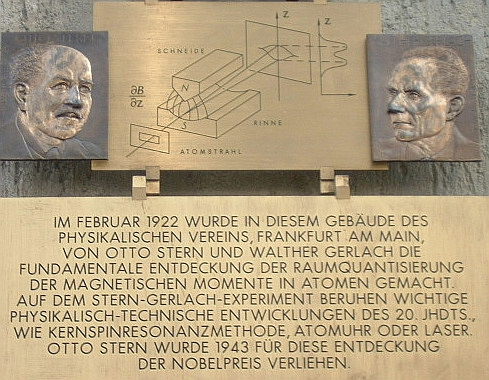
\includegraphics[scale=0.6]{SternGerlach2.jpg}\\
\textit{Plaque commémorative de la dite expérience avec les portraits de Otto Stern et Walther Gerlach. La plaque est située au siège de la Physikalische Verien à Francfort-sur-le-Main (Allemagne).}
\end{center}

\textit{Source : hptts://fr.wikipedia.org/wiki/Exp$\%$C3$\%$A9rience$\_$de$\_$Stern$\_$et$\_$Gerlach}\\
\hline
\end{tabular}\\

Nous allons utiliser un calcul classique en se basant sur le modèle planétaire de l'atome (modèle de Bohr). Ce modèle permet de montrer que le calcul classique ne peut décrire le phénomène de magnétisme quantique.

\section{Magnétisme classique}

La source revient à Ampère\footnote{\label{Ampère} André-Marie Ampère (1755 - 1836) est un mathématicien, physicien, chimiste et philosophe français. Son nom a été donné à l'unité du Système International pour l'intensité du courant électrique : l'Ampère (symbole A).} en 1811. Pour lui, la brique fondamentale du magnétisme est une boucle de courant ampérien. On utilise le modèle planétaire constitué d'un noyau et d'un seul électron en mouvement circulaire (dans la couche s). Soit un électron de masse $m$ et de charge $-e$\footnote{\label{élect} C'est la charge élémentaire de l'électron, où $e$ ayant pour valeur : $e = 1.602 \times 10^{(-19)}$ C (C pour Coulomb). Le proton et l'antiparticule de l'électron, le positron, ont tous les deux la valeur $+e$. \textit{Pour les curieux, la valeur exacte, fixée au 20 mai 2019 est : $e = 1.602~176~364 \times 10^{(-19)}$ Coulomb.}} ($e \sup 0$) autour d'un noyau fixé. Le système est rigide, le mouvement de l'électron résulte de deux forces opposées, centrifuges et électrostatique. Le moment est une constante (mouvement plan). Le mouvement est circulaire de rayon R ; la fréquence de mouvement de l'électron est de $10^{16}$ Hertz soit 10 PHz (Péta-Hertz). L'application du champ $\overrightarrow{B}$ en résulte une force $\overrightarrow{F}$ (force de Lorentz) :
\begin{equation*}
\overrightarrow{F} = e \overrightarrow{v} \wedge \overrightarrow{B}
\end{equation*}
En deux points, diamétralement opposés, l'électron se trouve soumis à deux forces opposées. Le mouvement interne étant supposé rigide, l'application du champ $\overrightarrow{B}$ provoque l'apparition d'un couple qui tend à faire orienter le plan de l'atome de façon à le rendre perpendiculaire à $\overrightarrow{B}$. On rappelle que :
\begin{equation*}
\frac{F_l}{F_{el}} \ll 1
\end{equation*}
Le champ $\overrightarrow{B}$ provoque une perturbation mineure du système atomique. De ce fait, une grandeur qui était une constante du mouvement (moment cinétique) ne l'est plus. Cependant, comme la perturbation est très faible, sa variation sera très lente. On dit que le moment cinétique $\overrightarrow{J}$ va varier dans le temps à cause du champ $\overrightarrow{B}$, c'est la précession de Larmor\footnote{\label{Armor} Nommée d'après le physicien, mathématicien et homme politique irlandais Joseph Larmor (1857 - 1942). À ne pas confondre avec l'Armor (qui désigne en breton le littoral) et aucun rapport avec Larmor-Plages (56, Morbihan).}.\\

Mais d'abord, jetons un \oe{}il à la géométrie utilisée pour le calcul du moment magnétique. Regardons le passage des coordonnées cartésiennes aux coordonnées cylindriques.\\

\begin{figure}[!h]
\begin{center}
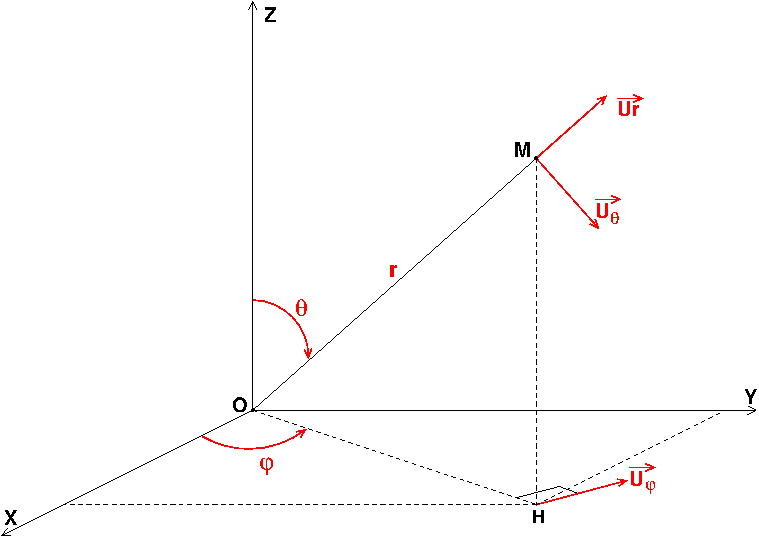
\includegraphics[scale=0.5]{cartesienne_a_cylindriques.png}
\caption{Passage des coordonnées cartésiennes aux coordonnées cylindriques.}
\label{coord1}
\end{center}
\end{figure}

\begin{center}
À noter, pour la suite, que : $\overrightarrow{R}$ est sur l'axe y et $\overrightarrow{v}$ correspond à $\overrightarrow{U_\varphi}$ sur le schéma.
\end{center}

\begin{center}
\[
\overrightarrow{R} = 
\left\lbrace
\begin{matrix}
R ~cos \varphi\\
R ~sin \varphi\\
0
\end{matrix}
\right\rbrace
~~;~~ \overrightarrow{v} =
\left\lbrace
\begin{matrix}
v ~cos (\varphi + \pi /2)\\
v ~sin (\varphi + \pi /2)\\
0
\end{matrix}
\right\rbrace
\]\\

\[
\overrightarrow{F_l} =
\left\lbrace
\begin{matrix}
e ~v ~B ~cos \varphi ~cos \theta\\
e ~v ~B ~cos \varphi ~sin \theta\\
0
\end{matrix}
\right\rbrace
=
\left\lbrace
\begin{matrix}
e ~R ~\omega ~B ~cos \varphi ~cos \theta\\
e ~R ~\omega ~B ~cos \varphi ~sin \theta\\
-e ~R ~\omega ~B ~cos \varphi ~sin \theta
\end{matrix}
\right\rbrace
\]
\end{center}

Le moment vaut donc :

\begin{center}
\[
\overrightarrow{M} = \overrightarrow{R} \wedge \overrightarrow{F} =
\left\lbrace
\begin{matrix}
-e ~R^2 ~B ~cos \varphi ~sin \varphi ~sin \theta\\
e ~R^2 ~cos^2 \varphi ~sin \theta\\
0
\end{matrix}
\right\rbrace
\]
\end{center}

En moyenne dans le temps sur le mouvement rapide, nous avons :

\begin{align*}
\int_0^{2\pi} cos \varphi ~sin \varphi ~d \varphi &= 0\\
cos^2 \varphi &= \frac{1 + cos 2 \varphi}{2}\\
\frac{1}{2\pi} \int_0^{2\pi} e~R~\omega^2~cos^2 \varphi~sin \theta &= \frac{1}{2} e ~R^2 ~\omega ~B ~sin \theta\\
\overrightarrow{M} &= 
\left\lbrace
\begin{matrix}
0 & \frac{1}{2} ~e ~R^2 ~\omega ~B ~sin \theta & 0\\
\end{matrix}
\right\rbrace
\end{align*}

$\overrightarrow{M} \perp \overrightarrow{B}$ et $\overrightarrow{M} \perp \overrightarrow{n}$ et le triède $\left( \overrightarrow{n}, \overrightarrow{M}, \overrightarrow{B} \right)$ est discret. On introduit $J = mvR = mR^2 \omega$, et il est oriente selon Oz. Alors : $\overrightarrow{M} = \frac{e}{2m} \overrightarrow{J} \wedge \overrightarrow{B}$. Plus généralement, pour une particule en mouvement circulaire de charge $Q$ et masse $m$ soumise à un champ $\overrightarrow{B}$ sur $\overrightarrow{M} = \frac{Q}{2m} \overrightarrow{J} \wedge \overrightarrow{B}$. Par identification avec $\overrightarrow{M} = \overrightarrow{\mu} \wedge \overrightarrow{B}$ nous en déduisons que $\overrightarrow{\mu} = \frac{e}{2m} \overrightarrow{J} = \gamma \overrightarrow{J}$ où $\gamma$ est le facteur gyromagnétique.\\

\begin{tabular}{|p{15cm}|}
\hline
\textbf{$\gamma$ le facteur gyromagnétique, aussi appelé rapport gyromagnétique}\\

Il s'agit d'un rapport entre le moment magnétique et le moment cinétique d'une particule. Son unité dans le Système International est le Coulomb par Kilogramme ($C.kg^{-1}$) mais en pratique, il est souvent exprimé en Mégahertz par tesla ($MHz.T^{-1}$), car il est plus commun d'avoir : $\frac{\gamma}{2\pi}$.\\

\textit{Source : hptts://fr.wikipedia.org/wiki/Rapport$\_$gyromagn$\%$C3$\%$A9tique}\\
\hline
\end{tabular}\\

Dans notre cas $\gamma < 0$ car $e < 0$. Donc $\overrightarrow{\mu}$ le moment magnétique et $\overrightarrow{J}$ le moment cinétique sont de sens opposés. Comme $J \approx \hbar$ ; il est usuel d'avoir l'unité naturelle du moment magnétique :
\begin{equation*}
µB = \frac{e \hbar}{2m}
\end{equation*}
\textbf{C'est le magnétisme de Bohr.} Ce couple tend à aligner le moment dans la direction du champ magnétique. Quand le système (atome + champ) est isolé, son énergie est constante, et donc $\theta$ est constant aussi : c'est pourquoi $\overrightarrow{J}$ et $\overrightarrow{\mu}$ précesse autour de $\overrightarrow{B}$. Si maintenant, on applique un couple pour changer l'angle $\theta$ à $\theta + d\theta$, le travail reçu ou cédé par le système sera :
\begin{center}
$dW = µB ~sin \theta ~d\theta$
\[
\begin{matrix}
dW > 0 & d\theta > 0\\
dW < 0 & d\theta < 0
\end{matrix}
\]
\end{center}
La variation correspondante de l'énergie du système est égale à :
\begin{center}
$dW = dE = \vert \mu \vert B ~sin\theta ~d\theta$\\
$dE = -d(\overrightarrow{\mu} \wedge \overrightarrow{B})$\\
$E = -\overrightarrow{\mu} \overrightarrow{B} + \text{cst}$
\end{center}
L'expression de l'énergie montre que la position d'équilibre stable correspond à l'angle $\theta = 0$. $E$ est très bas. Du point de vue macroscopique, le moment magnétique d'un circuit du surface $S$ est parcouru par un courant $I$ est donnée par l'expression : $IS$. Pour la boucle atomique : $I = \frac{dq}{dt} = e \nu$ et $S = \pi R^2$. Donc : $IS = e \nu \pi R^2 = \frac{e}{2} 2 \pi \nu R^2 \omega = \frac{e}{2m} m R^2 \omega = \frac{e}{2m} \overrightarrow{J} = \overrightarrow{\mu}$. Les deux définitions sont identiques ! \textbf{Remarque :} nous retiendrons que la forme du couplage entre un moment magnétique $\overrightarrow{\mu}$ et un champ magnétique $\overrightarrow{B}$ est donné par : $V_{moy} = -\mu B$. 

\section{La précession de Larmor}

On décrit dans cette partie la dynamique du système (atome + champ magnétique). En présence du champ magnétique $\overrightarrow{B}$ et d'après le théorème du moment cinétique.
\begin{equation*}
\frac{d \overrightarrow{J}}{dt} = \overrightarrow{\mu} \wedge \overrightarrow{B} = \frac{e}{2m} \overrightarrow{J} \wedge \overrightarrow{B}
\end{equation*}

Si $B = 0$ ou $\frac{d \overrightarrow{J}}{dt} = 0$, alors $\overrightarrow{J}$ est une constante du mouvement. Cette équation décrit un mouvement gyroscopique. Le vecteur $\overrightarrow{J}$, constante en norme, fait un angle constant avec la direction du champ magnétique et tourne autour de cette dernière. Un tel mouvement s'appelle précession. Le vecteur $\overrightarrow{J}$ tourne à la pulsation $\omega_{L}$ appelée pulsation de Larmor !

\begin{equation*}
\omega_{L} = \vert \gamma \vert B = \frac{\vert e \vert}{2m} B = \hbar^{-1} \vert \mu_{B} \vert B
\end{equation*}

Si nous écrivons :
\begin{equation*}
\overrightarrow{J} \cdot \frac{dJ}{dt} = \overrightarrow{J} \cdot \gamma \overrightarrow{J} \wedge \overrightarrow{B} = 0 = \frac{1}{2} \frac{d}{dt} (J)^2
\end{equation*}

$\Vert J^2 \Vert = $ constante. Par contre, nous savons que : $\frac{d \overrightarrow{J}}{dt} \perp B$. D'où $J_z \Vert B$ est constant. $(B = (0,0,B_z ))$.

\begin{center}
$J^2 (t) = J^2 (t=0)$ et $J_z (t) = J_z (t=0)$\\
D'où $J^2_x (t) + J^2_y (t) = J^2 (t=0) - J_x^2 (t=0)$
\end{center}
$\overrightarrow{J}(t)$ tourne autour de $\overrightarrow{B}$ et fait un angle $x .\theta$ avec $B$. ($\overrightarrow{\mu}$ fait un angle $\theta$ avec $\overrightarrow{B}$) et $cos \theta = \frac{J_z (t=0)}{\vert J \vert (t=0)}$. Le calcul des composantes $J_x (t)$ et $J_y (t)$ : $\frac{dJ_x}{dt} = \gamma B J_y$ et $\frac{dJ_y}{dt} = -\gamma B J_x$. En introduisant : $J_+ (t) = J_x + iJ_y$ et $J_-(t) = J_x -iJ_y$, nous avons donc :
\begin{center}
$\frac{d}{dt} J_+ (t) = i \omega_{L} J_+ (t)$ avec $J_+ (t) = J_+ (t=0) ~exp(-i \omega_{L} t)$\\
$\frac{d}{dt} J_- (t) = i \omega_{L} J_- (t)$ avec $J_- (t) = J_- (t=0) ~exp(-i \omega_{L} t)$
\end{center}
À noter que : $J_+ (0) = J_- (0)$.

\section{Quantification du moment cinétique}
\subsection{Description de l'appareil}

L'expérience de Stern et Gerlach a permis de mettre en évidence la quantification du moment cinétique. Son principe repose sur l'étude de la déviation d'un atome paramagnétique sous l'effet d'un champ magnétique homogène.\\

\begin{center}
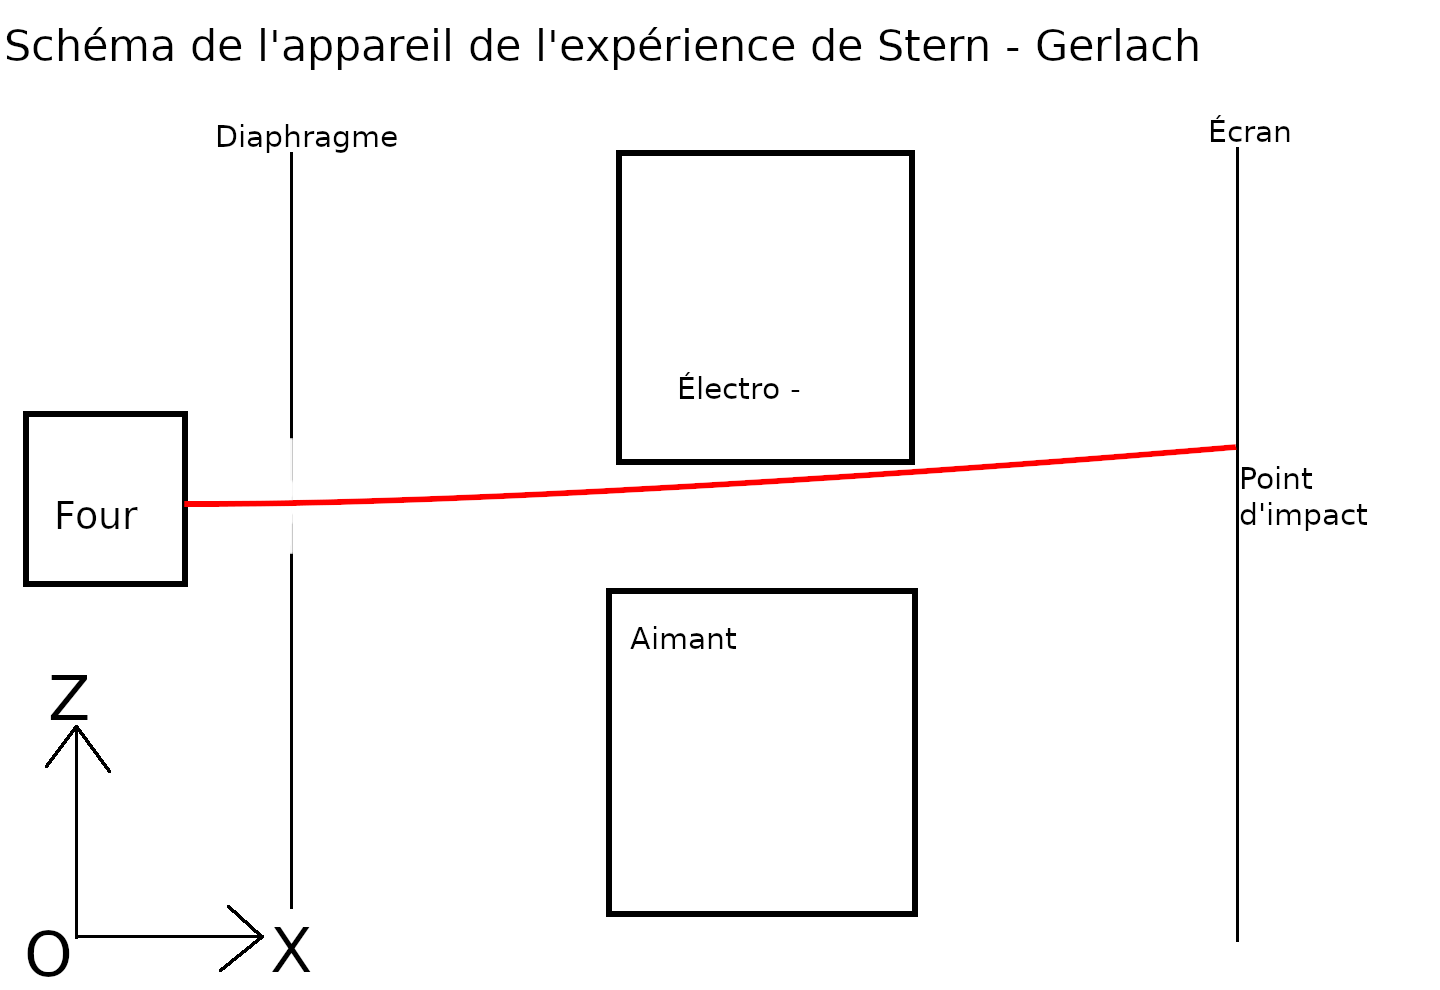
\includegraphics[scale=0.6]{exp_stern_gerlach_zx_pov_y.png}
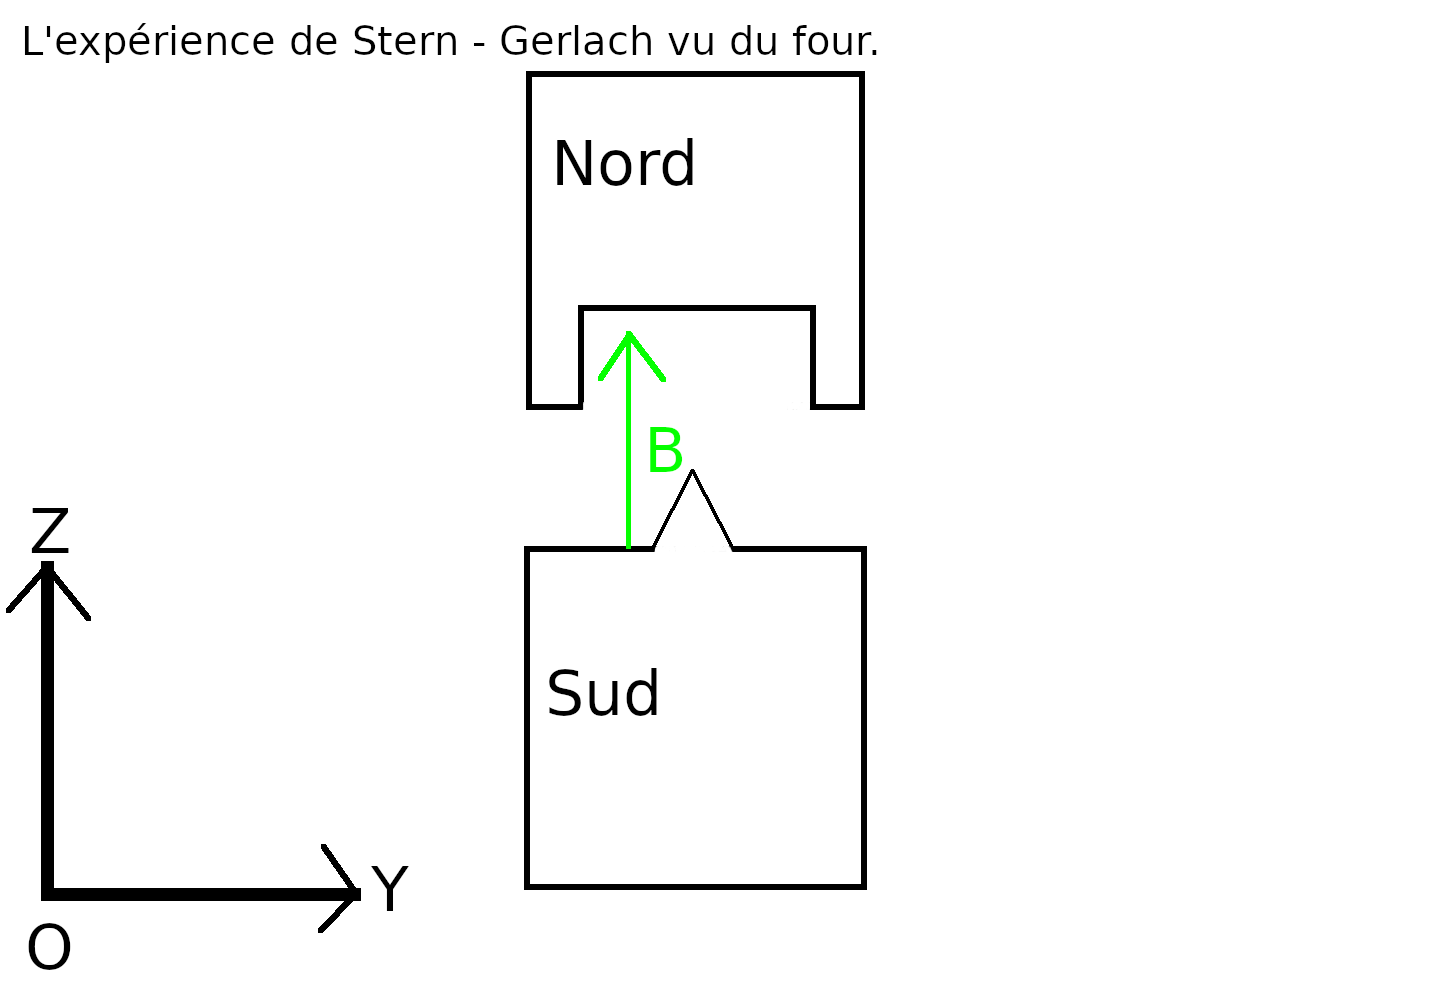
\includegraphics[scale=0.6]{exp_stern_gerlach_zy_pov_x.png}
\end{center}

$B_z$ est positif : $\frac{\partial B}{\partial z} < 0$
Le plan Oxz est un plan de symétrie. $B_x = 0$ ; $\frac{\partial B_y}{\partial y} \neq 0$ ; $\text{div} \overrightarrow{B} = 0$.\\

Mais comment fonctionne cette expérience ?

Les atomes d'argent sont issus d'un four, puis un diaphragme sélectionne les atomes dont la vitesse est parallèle à Ox. Ensuite, les atomes traversent une zone où règne un champ magnétique homogène. Le champ magnétique $B$ a les caractéristiques suivantes :

- sa plus grande composante est selon l'axe z ;

- il est le même en tout point d'un parallèle à l'axe x.

\subsection{Calcul classique de la déviation}
Les atomes d'argent sont neutres et à l'état fondamental. Ils possèdent un moment magnétique permanent $\overrightarrow{\mu}$. Dans la zone où règne le champ magnétique, les atomes d'argent se trouvent soumis à une force :
\begin{equation*}
\overrightarrow{F} = -\overrightarrow{\text{grad}} W ~~;~~ W = - \overrightarrow{\mu} \overrightarrow{B}
\end{equation*}

\paragraph*{Remarque :}

pour un atome, il y a deux origines de l'existence d'un moment magnétique $\overrightarrow{\mu}$ :

- le moment des électrons autour du noyau qui donnent lieu au moment cinétique orbital ;

- le moment cinétique intrinsèque, appelé le spin.

\begin{equation*}
\overrightarrow{\mu} = \gamma \overrightarrow{J} ~~;~~ \overrightarrow{J} = \overrightarrow{L} + \overrightarrow{S} ~~;~~ \overrightarrow{\mu} = \gamma (\overrightarrow{L} + \overrightarrow{S})
\end{equation*}

Avec $\overrightarrow{L}$ le moment cinétique orbital et $\overrightarrow{S}$ le spin.

À l'entrée de la zone où règne le champ magnétique, les moments cinétiques des atomes d'argent sont orientés de manières aléatoire ($\theta$ varie de 0 à $\pi$). On étudie l'effet du champ magnétique sur le cas d'un atome dont le moment magnétique a une orientation quelconque. On sait que :
\begin{center}
$\overrightarrow{F} = - \overrightarrow{\text{grad}} W = - \overrightarrow{\text{grad}} \overrightarrow{\mu} \overrightarrow{B}$\\
$\braket{\mu_x} = \braket{\mu_y} = 0$
\end{center}

\paragraph*{Rappel :}

$\mu_x \propto ~cos(\omega t + \varphi)$ et $\mu_y \propto ~sin(\omega t + \varphi)$

$\overrightarrow{F}$ a une seule composante selon Oz : $F_z = \mu_z \overrightarrow{\text{grad}} B_z = \mu_z \frac{\partial B_z}{\partial z} \overrightarrow{k}$

$B_z$ est indépendante de x et y. La force exercée sur les atomes d'argent est proportionnel à $\mu_z$. Comme cette force est responsable de la déviation des atomes d'argent, mesurer la déviation revient à mesurer $\mu_z$. Comme $\overrightarrow{\mu}$ peut être orienté de manière aléatoire, $\mu_z$ peut prendre toutes les valeurs entre $- \vert \mu \vert$ et $+\mu$, aussi on s'attend à ce que les atomes d'argent se répartissent de manière continue sur l'écran et former une tâche longitudinale selon Oz et symétrique au centre.

\subsection{Résultat et conclusion}

$\blacktriangleright$ Les résultats de l'expérience de Stern et Gerlach contredisent les prévisions de la physique classique.

$\blacktriangleright$ Ces résultats montrent deux tâches distinctes symétriques au centre de l'écran.

\begin{figure}[!h]
\centering
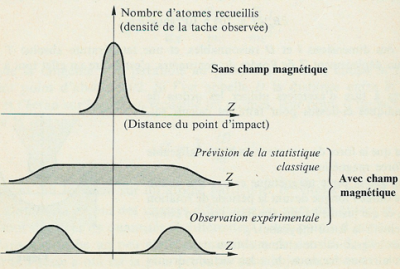
\includegraphics[scale=1]{results-stern-gerlach.png}
\caption{Les différents résultats théoriques et expérimental de l'expérience de Stern et Gerlach.}
\label{fig:resultSG1}
\end{figure}

Pour interpréter ces résultats, on distingue entre les degrés de liberté internes (le moment magnétique et son interaction avec le champ...) qu'on doit traiter quantiquement et les degrés de liberté externe (position et impulsion de l'atome dans l'espace) qu'on peut traiter classiquement (\textit{passage vu en TD}).

Les conclusions de l'expérience de Stern et Gerlach nous conduisent à conclure que la projection du moment cinétique selon Oz possède deux valeurs uniquement. Ces valeurs sont distinctes. Le schéma classique est donc erroné !

- $\mu_z$ ne peut prendre que 2 valeurs, idem pour $J_z$.

- $\mu_z$ et $J_z$ sont deux grandeurs quantiques.

- Pour le moment, on admet que les valeurs de $J_z$ sont $\pm \frac{h}{2}$ et que le moment cinétique de l'atome d'argent correspond au moment cinétique du spin.

\subsection{Description théorique}

Nous savons déjà (postulat 2) que toute grandeur physique mesurable lui correspond une observable. Cette observable n'est pas forcément un ensemble complet d'observables qui commutent. Ainsi, on associe l'opérateur vectoriel $\overrightarrow{S}(S_x , S_y , S_z)$ au spin de l'atome $\mathfrak{S}$\footnote{Oui, c'est un S !}. $S_x$, $S_y$ et $S_z$ sont des observables et aussi des ensembles complet d'observables qui commutent.

\subsection{L'observable $S_z$ et l'espace des états du spin}

$S_z$ est l'observable associée à la composante selon Oz du spin atomique $\mathfrak{S}_z$. Les résultats de Stern et Gerlach montrent que les valeurs propres  de $S_z$ sont $+\frac{\hbar}{2}$ et $-\frac{\hbar}{2}$. Nous admettons que ces valeurs propres ne sont pas dégénérées, d'où :
\begin{align*}
+ \frac{\hbar}{2} \longrightarrow \ket{z+} &= \ket+ \\
- \frac{\hbar}{2} \longrightarrow \ket{z-} &= \ket-
\end{align*}
\begin{center}
$S_z \ket+ = \frac{\hbar}{2} \ket+$ et $S_z \ket- = \frac{-\hbar}{2} \ket-$
\end{center}

$\left\lbrace \ket+ , \ket- \right\rbrace$ forment une base de l'espace des états du spin.

\begin{center}
$\braket{+|+} = \braket{-|-} = 1$ et $\braket{-|+} = 0$
\end{center}
Ainsi, tout état de l'espace des états du spin est décrit comme une superposition de ces deux états.

Soit $\ket\Psi ~\in~ \mathcal{E}_s$ ; $\ket\Psi = \alpha \ket+ + \beta \ket-$ ; $\vert \alpha \vert^2 + \vert \beta \vert^2 = 1$

Dans la base $\left\lbrace \ket+ ; \ket- \right\rbrace$ :
\begin{center}
\[
S_z = \frac{\hbar}{2}
\left\lbrace
\begin{matrix}
1 & 0\\
0 & -1
\end{matrix}
\right\rbrace
= \frac{\hbar}{2} \sigma_z
\]
\end{center}
où $\sigma_z$ est une matrice de Pauli.

\subsection{Les autres composantes $S_x$ et $S_y$}

$S_x$ est l'observable associée à $\mathfrak{S}_x$ ;

$S_y$ est l'observable associée à $\mathfrak{S}_y$.

On a :
\begin{center}
\[
S_x = \frac{\hbar}{2}
\left\lbrace
\begin{matrix}
0 & 1\\
1 & 0
\end{matrix}
\right\rbrace
= \frac{\hbar}{2} \sigma_x
\]\\

\[
S_y = \frac{\hbar}{2}
\left\lbrace
\begin{matrix}
0 & -i\\
i & 0
\end{matrix}
\right\rbrace
= \frac{\hbar}{2} \sigma_y
\]
\end{center}

$\sigma_x$ et $\sigma_y$ sont deux autres matrices de Pauli. On peut considérer une composante de $\overrightarrow{S}$ selon le sens $\overrightarrow{u}$ décrit par ($\theta$ et $\varphi$).

\begin{center}
\[
\overrightarrow{u} =
\left\lbrace
\begin{matrix}
sin \theta ~cos \varphi \\
sin \theta ~sin \varphi \\
cos \theta
\end{matrix}
\right\rbrace
\]
\end{center}

\begin{center}
\[
S_u = \overrightarrow{S} \cdot \overrightarrow{u} = sin \theta ~cos \varphi + S_x + sin \theta ~sin \varphi S_y + cos \theta S_z
\]\\

\[
S_u = \frac{\hbar}{2}
\left[
\left(
\begin{matrix}
0 & sin \theta ~cos \varphi \\
sin \theta ~cos \varphi & 0
\end{matrix}
\right)
+
\left(
\begin{matrix}
0 & -i ~sin \theta ~sin \varphi \\
i ~sin \theta ~sin \varphi & 0
\end{matrix}
\right)
+
\left(
\begin{matrix}
cos \theta & 0 \\
0 & -cos \theta
\end{matrix}
\right)
\right]
\]\\

\[
S_u = \frac{\hbar}{2}
\left(
\begin{matrix}
cos \theta & sin \theta ~e^{-i \varphi} \\
sin \theta ~e^{i \varphi} & -cos \theta
\end{matrix}
\right)
\]
\end{center}

\begin{tabular}{|p{15cm}|}

\hline
\textbf{Exercice d'application pour la maison :}\\
\hline
- chercher les valeurs propres de $S_x$, $S_y$, $S_z$ ;

- trouver les vecteurs propres dans la base $\lbrace \ket+ ; \ket- \rbrace$ ;

- donner chaque matrice dans la base des vecteurs propres.\\
\hline
\end{tabular}

\subsection{Évolution d'un spin 1/2 dans un champ magnétique uniforme}
\subsubsection{A : Hamiltonien d'intersection et équation de Schrödinger}

Considérons une particule d'un spin $\frac{1}{2}$ plongée dans un champ magnétique uniforme $B_0 \overrightarrow{k}$ (selon Oz). Le potentiel d'interaction du moment magnétique avec le champ $B$ est $W$ :
\begin{equation*}
W = -\mu B = -\mu_{B} B_0 = -\gamma S_z B_0
\end{equation*}
Soit $\omega_0 = -\gamma B_0$ ($\gamma < 0$ ; $\omega_0 > 0$)
\begin{equation*}
H = \omega_0 S_z = \frac{\hbar}{2} \omega_0 \sigma_z
\end{equation*}

$H$ ne dépend pas du temps, d'où l'équation de Schrödinger se résume à l'équation aux valeurs propres. On sait que $[H,S_z] = 0$. $H$ et $S_z$ ont les mêmes vecteurs propres.

\begin{align*}
H_0 \ket+ &= \frac{\hbar}{2} \omega_0 \ket+ \\
H_0 \ket- &= \frac{-\hbar}{2} \omega_0 \ket-
\end{align*}

$S_z$ est une constante du mouvement : $\frac{d}{dt} \braket{S_z} = 0$ et $\braket{S_z} = $constante. Ce n'est pas le cas pour $S_x$ et $S_y$. Vérifions $[S_x, S_z] [S_y, S_z]$ et $[S_x, S_y]$.

\paragraph*{Rappel : }

le choix de l'orientation de $B$ est arbitraire, on peut choisir $B$ selon Ox, Oy ou selon la direction d'un vecteur $\overrightarrow{u}$ quelconque. Dans toute les situations $H$ possède deux valeurs propres.

\begin{align*}
E_+ &= \frac{\hbar}{2} \omega_0 \\
E_- &= -\frac{\hbar}{2} \omega_0
\end{align*}

Les vecteurs propres dépendent de l'orientation de $\overrightarrow{B}$.

\subsubsection{B : Précession de Larmor}

Considérons une particule de spin $\frac{1}{2}$ plongée dans un champ magnétique uniforme $\overrightarrow{B} = B_0 \overrightarrow{k}$.
\begin{equation*}
H = -\overrightarrow{\mu} \overrightarrow{B} = \omega_0 S_z
\end{equation*}
Les états $\ket+$ et $\ket-$ sont des vecteurs propres associés aux valeurs propres $+\frac{\hbar}{2} \omega_0$ et $-\frac{\hbar}{2} \omega_0$ respectivement.

Considérons une particule dans l'état $\ket{\Psi(0)} = \ket{U_+}$ où $\ket{U_+}$ est un vecteur propre de $S_u$ associé à $\frac{\hbar}{2}$, idem pour $\ket{U_-}$ mais avec $-\frac{\hbar}{2}$.

\begin{align*}
\ket{U_+} &= cos \frac{\theta}{2} ~exp \left(-i \frac{\varphi}{2} \right) \ket+ + sin \frac{\theta}{2} exp \left(i \frac{\theta}{2} \right) \ket- \\
\ket{U_-} &= -sin \frac{\theta}{2} ~exp \left(-i \frac{\varphi}{2} \right) \ket+ + cos \frac{\theta}{2} exp \left(i \frac{\theta}{2} \right) \ket-
\end{align*}

À $t=0$ : $\ket{\Psi (t)} = \ket{U_+}$ ;\\

À $t$ : $\ket{\Psi (t)} = cos \frac{\theta}{2} ~exp \left(-i \frac{\theta}{2} \right) ~exp \left(-i \frac{E_+ t}{\hbar} \right) \ket{U_+} + sin \frac{\theta}{2} ~exp \left(+i \frac{\varphi}{2} \right) ~exp \left(-i \frac{E_- t}{\hbar} \right) \ket-$ ;\\

Donc : $\ket{\Psi (t)} = cos \frac{\theta}{2} ~exp \left(+i \frac{\varphi + \omega_0 t}{2} \right) \ket+ + sin \frac{\theta}{2} ~exp \left(+i \frac{\varphi + \omega_0 t}{2} \right) \ket-$\\

En comparant $\ket{\Psi (t=0)}$ et $\ket{\Psi (t)}$, nous remarquons que l'orientation du vecteur $\overrightarrow{u}$ garde le même écart angulaire avec l'axe Oz. Cependant l'angle $\varphi$ varie à la pulsation $\omega_0 = \vert \gamma \vert B_0$. Cette variation montre que le vecteur $\overrightarrow{u}$ et donc l'état $\ket{U_+}$ de $S_z$ précesse autour de Oz (champ magnétique). On retrouve le mouvement prédit par la mécanique classique. Bien évidemment, $S_z$ est une constante du mouvement.

\begin{align*}
\braket{\Psi (t) | S_z | \Psi (t)} &= \frac{\hbar}{2} ~cos^2 \frac{\theta}{2} + \frac{\hbar}{2} ~sin^2 \frac{\hbar}{2} = \frac{\hbar}{2}\\
\\
\braket{\Psi(0) | S_z | \Psi(0)} &= \frac{\hbar}{2} ~cos^2 \frac{\theta}{2} + \frac{\hbar}{2} ~sin^2 \frac{\hbar}{2} = \frac{\hbar}{2}
\end{align*}

$S_x$ et $S_y$ ne sont pas des constantes de mouvement. Calcul des valeurs moyennes de $\braket{S_x}(t)$ et $\braket{S_y}(t)$.

\begin{center}
$\braket{\Psi (t) \vert S_x \vert \Psi (t)} = \frac{\hbar}{2} ~cos \left( \varphi + \omega_0 t \right)$\\
$\braket{\Psi (t) \vert S_y \vert \Psi (t)} = \frac{\hbar}{2} ~sin \theta ~sin \left( \varphi + \omega_0 t \right)$
\end{center}

Les valeurs propres $\braket{S_x} (t)$ et $\braket{S_y} (t)$ se comportent comme le prédit la théorie classique, elle précessent autour de l'axe du champ $\overrightarrow{B}$ à la pulsation $\omega_0 = \vert \omega \vert B_0$.

\chapter{OUTILS MATHÉMATIQUES 2}

\section{Introduction de bases n'appartenant pas à $\mathfrak{F}$}

\subsection{Onde plane}

Une onde plane de vecteur d'onde $\overrightarrow{k} = \frac{\overrightarrow{P}}{\hbar}$ (d'impulsion $\overrightarrow{p}$) est décrite par la fonction :
\begin{equation*}
V_p (x) = \frac{1}{\sqrt{2 \pi \hbar}} ~exp \left( i \frac{\overrightarrow{p} \cdot \overrightarrow{x}}{\hbar} \right)
\end{equation*}
On remarque que $V_p (x)$ est une fonction qui n'est pas de carré sommable et donc n'appartient pas à $\mathfrak{F}$.

$\lbrace V_p (x) \rbrace$ est une base continue de fonctions d'ondes planes ; p variant de $- \infty$ à $+ \infty$ de manière continue : $\overrightarrow{p} ~\in~ ]-\infty ; + \infty[$.

\subsection{Rappel sur la transformée de Fourier}

Soit $\Psi (x)$ est une fonction d'onde, sa transformée de Fourier $\overline{\Psi} (p)$ est définie par :

\begin{equation*}
\overline{\Psi} (p) = \frac{1}{\sqrt{2 \pi \hbar}} \int_{- \infty}^{+ \infty} exp \left( \frac{-i px}{\hbar} \right) \Psi (x) dx = \int_{- \infty}^{+ \infty} V_p^{*} (x) \Psi (x) dx 
\end{equation*}

la formule inverse :

\begin{equation*}
\Psi (x) = \int_{-\infty}^{+\infty} V_p (x) \overline{\Psi} (p) ~dp = \frac{1}{\sqrt{2 \pi \hbar}} \int_{-\infty}^{+\infty} ~exp \left( i \frac{px}{\hbar} \right) \overline{\Psi}(p) ~dp
\end{equation*}

La dernière relation exprime que toute fonction d'onde $\Psi (t)$ est développable d'une seule manière sur les fonctions $V_p (x)$ ; l'indice $p$ varie de façon continue.

$\overline{\Psi} (p)$, la transformée de $\Psi (x)$, est la composante de $\Psi (x)$ sur l'onde plane $\Psi_p (x)$. $\overline{\Psi} (p)$ est donnée par le produit scalaire de $\Psi (x)$ sur l'onde plane $V_p (x)$. Dans le cas des bases continue, on remplace la somme par l'intégration sur $dp$.

\subsection{La base $\lbrace v_p (x) \rbrace$ vérifie la relation de fermeture}

Soit $\delta (x-x_0)$ est la fonction de Dirac.
\begin{center}
$\delta (x-x_0) = 0$ si $x \neq x_0$\\
$\delta (x-x_0) = \infty$ si $x = x_0$
\end{center}

Soit $\delta_{x_0} (p)$ est la transformée de Fourier de $\delta (x-x_0)$.
\begin{equation*}
\delta_{x_0} (p) = \int_{- \infty}^{+ \infty} V_p^* (x) \delta (x-x_0) dx = \frac{1}{\sqrt{2 \pi \hbar}} \int_{- \infty}^{+ \infty} ~exp \left( -i \frac{px}{\hbar} \right) \delta (x-x_0) = \frac{1}{\sqrt{2 \pi \hbar}} ~exp \left( -i \frac{px_0}{\hbar} \right)
\end{equation*}

La formule inverse :
\begin{align*}
\delta (x-x_0) &= \int_{- \infty}^{+ \infty} \frac{1}{(\sqrt{2 \pi \hbar})^2} ~exp \left( i \frac{px}{\hbar} \right) ~exp \left( -i \frac{px_0}{\hbar} \right) dp \\
&= \frac{1}{(\sqrt{2 \pi \hbar})^2} \int_{- \infty}^{+ \infty} ~exp \left( i (x-x_0)p \right) dp\\
&= \int_{- \infty}^{+ \infty} V_p^* (x_0) V_p (x) dp
\end{align*}

Cette relation constitue la relation de fermeture dans la base $\lbrace V_p (x) \rbrace$.

Calcul du produit scalaire $\left( V_p (x), V_{p'} (x) \right)$.

\begin{align*}
\left( V_p (x), V_{p'} (x) \right) &= \frac{1}{\sqrt{2 \pi \hbar}} \int_{- \infty}^{+ \infty} ~exp \left( i \frac{(p'-p)x}{\hbar} \right) dx = \delta (p-p')\\
\delta (p-p') &= 0 ~\text{si}~ p \neq p'\\
&= \infty ~\text{si}~ p = p'
\end{align*}

Dans un abus de langage, on désigne cette relation comme une relation d'orthonormalisation. On dit aussi que les fonctions $V_p (x)$ sont orthonormées au sens du Dirac.

\subsection{La généralisation aux fonctions à trois dimensions}

\begin{align*}
V_p (\overrightarrow{x}) &= \frac{1}{(2 \pi \hbar)^{3/2}} ~exp \left( i \frac{\overrightarrow{p} \cdot \overrightarrow{x}}{\hbar} \right)\\
\Psi (\overrightarrow{x}) &= \int_{- \infty}^{+ \infty} d^3 p \overline{\Psi} (p) V_p (\overrightarrow{x})\\
&= \int_{- \infty}^{+ \infty} d^3 p V_p^* (\overrightarrow{x}) V_p (\overrightarrow{x'})\\
&= \delta (\overrightarrow{x} - \overrightarrow{x'})\\
\overline{\Psi} (p) &= \int_{- \infty}^{+ \infty} V_p^* (\overrightarrow{x}) \Psi (\overrightarrow{x}) d^3 x\\
&= \int_{- \infty}^{+ \infty} d^3 x V_p^* (\overrightarrow{x}) V_{p'} (\overrightarrow{x})\\
&= \delta (\overrightarrow{p} - \overrightarrow{p'})
\end{align*}

La correspondance entre la base discrète et la base continue :
\begin{center}
$i \longleftrightarrow p$ ; $\sum\limits_i \longleftrightarrow \int_{- \infty}^{+ \infty} d^3 p$ et $\delta_{ij} \longleftrightarrow \delta (p-p')$
\end{center}

\section{La fonction delta}

\subsection{Introduction}

Considérons la fonction $\delta^{\varepsilon} (x)$ donnée par le schéma :

% reproduire le schéma dans le cours !

\begin{center}
$\delta^{\varepsilon} (x) = \frac{1}{\varepsilon}$ si $-\frac{\varepsilon}{2} \leq x \leq \frac{\varepsilon}{2}$\\
$\delta^{\varepsilon} (x) = 0$ si $\vert x \vert > \frac{\varepsilon}{2}$\\
$\varepsilon$ est positif.
\end{center}

Calculons l'intégrale : $\int_{- \infty}^{+ \infty} dx \delta^{\varepsilon} f(x)$

$f(x)$ est une fonction bien définie au point $x=0$. Si $\varepsilon$ est suffisamment petit, la variation de $f(x)$ dans l'intervalle $\left[ -\frac{\varepsilon}{2} ; \frac{\varepsilon}{2} \right]$ est négligeable et $f(x) = f(0)$.\\

Ainsi : $\int_{- }^{+ \infty} \delta^{\varepsilon} (x) f(x) dx = \int_{- \frac{\varepsilon}{2}}^{+ \frac{\varepsilon}{2}} \delta^{\varepsilon} (x) f(x) dx = f(0) \int_{- \frac{\varepsilon}{2}}^{+ \frac{\varepsilon}{2}} \delta^{\varepsilon} (x) dx = f(0)$\\

L'approximation est d'autant meilleur que $\varepsilon$ est petit. Nous pouvons, donc, à la limite $\varepsilon = 0$, définir la fonction $\delta (x)$ (delta) par la relation :
\begin{equation*}
\int_{- \infty}^{+ \infty} f(x) \delta (x) = f(0)
\end{equation*}
Cette relation est valable pour toute fonction définie à l'origine. De façon générale, la fonction $\delta (x-x_0)$ est définie, telle que :
\begin{equation*}
\int_{- \infty}^{+ \infty} \delta (x-x_0) f(x) dx = f(x_0)
\end{equation*}

\subsection{Propriété de la fonction delta}

$\blacktriangleright \delta(-x) = \delta (x)$\\

$\blacktriangleright \delta (cx) = \frac{1}{\vert c \vert} \delta (x)$\\

$\blacktriangleright x \delta(x) = 0 $ / $x \delta (x-x_0) = x_0 \delta (x-x_0)$\\

$\blacktriangleright \int_{- \infty}^{+ \infty} \delta (x-y) \delta (x-z) dx = \delta (y-z)$\\

Considérons un ensemble de fonction de $\overrightarrow{r} ~ \left\lbrace \xi_{\overrightarrow{r_0}} (\overrightarrow{x}) \right\rbrace $ repérées par l'indice continue $\overrightarrow{r_0} (x_0 , y_0 , z_0)$ et définie par :

\begin{equation*}
\xi_{\overrightarrow{r_0}} (\overrightarrow{r}) = \delta (\overrightarrow{r} - \overrightarrow{r_0})
\end{equation*}

$\left\lbrace \xi_{\overrightarrow{r_0}} (\overrightarrow{x}) \right\rbrace$ représente l'ensemble des fonctions delta centrées aux différentes positions $\overrightarrow{r_0}$ de l'espace ($\overrightarrow{r_0}$ est une variable continue) ; $ \xi_{\overrightarrow{r_0}} (\overrightarrow{x})$ évidemment n'est pas de carré sommable et donc n'appartient pas à $\mathfrak{F}$.

\begin{align*}
\int_{- \infty}^{+ \infty} \vert \delta (x) \vert^2 &= \delta (0) \longrightarrow \text{de hauteur} ~\frac{1}{\varepsilon} ~\text{et}~ \varepsilon \longrightarrow 0\\
&= \infty
\end{align*}

Considérons les égalités suivantes :
\begin{align*}
\Psi (\overrightarrow{r}) &= \int_{- \infty}^{+ \infty} \delta (\overrightarrow{r} - \overrightarrow{r_0}) \Psi (\overrightarrow{r_0}) d^3 \overrightarrow{r_0}\\
\Psi (\overrightarrow{r_0}) &= \int_{- \infty}^{+ \infty} \delta (\overrightarrow{r} - \overrightarrow{r_0}) \Psi (\overrightarrow{r}) d^3 \overrightarrow{r}
\end{align*}
ou
\begin{align*}
\Psi (\overrightarrow{r}) &= \int_{- \infty}^{+ \infty} \xi_{\overrightarrow{r_0}} (\overrightarrow{r}) \Psi (\overrightarrow{r_0}) d^3 \overrightarrow{r_0}\\
\Psi (\overrightarrow{r_0}) &= \int_{- \infty}^{+ \infty} \xi_{\overrightarrow{r_0}} (\overrightarrow{r}) \Psi (\overrightarrow{r}) d^3 \overrightarrow{r}\\
&= \left( \xi_{\overrightarrow{r_0}} (\overrightarrow{r}) ; \Psi (\overrightarrow{r}) \right)
\end{align*}
Les deux dernières relations expriment que toute fonction $\Psi (\overrightarrow{r}) ~\in~ \mathfrak{F}$ est développable de façon unique sur les fonctions $\xi_{\overrightarrow{r_0}}$ ($\overrightarrow{r_0}$ est une variable continue). $\Psi (\overrightarrow{r_0})$ est la composante de $\Psi (\overrightarrow{r})$ sur la fonction $\xi_{\overrightarrow{r_0}}$.

Relation de fermeture :
\begin{equation*}
\int_{- \infty}^{+ \infty} \xi_{\overrightarrow{r_0}}^* (\overrightarrow{r}) \xi_{\overrightarrow{r_0}} (\overrightarrow{r'}) d^3 \overrightarrow{r_0} = \delta (\overrightarrow{r} - \overrightarrow{r'})
\end{equation*}

Relation d'orthogonalisation :
\begin{equation*}
\int_{- \infty}^{+ \infty} \xi_{\overrightarrow{r_0}}^* (\overrightarrow{r}) \xi_{\overrightarrow{r_0 '}} (\overrightarrow{r}) d^3 \overrightarrow{r_0} = \delta (\overrightarrow{r_0} - \overrightarrow{r_0 '})
\end{equation*}

Orthogonalisation au sens de Dirac. La correspondance entre la base discrète et la base continue :
\begin{center}
$i \longleftrightarrow \overrightarrow{r_0}$ ; $\sum\limits_i \longleftrightarrow \int_{- \infty}^{+ \infty} d^3 \overrightarrow{r_0}$ et $\delta_{ij} \longleftrightarrow \delta (\overrightarrow{r_0}-\overrightarrow{r_0}')$
\end{center}

\section{Deux exemples important de représentations et d'observables}

\subsection{Les représentation $\lbrace \ket r \rbrace$ et $\lbrace \ket p \rbrace$}

\subsubsection{A : Définition}

On associe par définition la fonction :
\begin{center}
$\xi_{\overrightarrow{r_0}} (\overrightarrow{r}) \longrightarrow \ket{\overrightarrow{r_0}}$\\
$V_{\overrightarrow{p_0}} (\overrightarrow{p}) \longrightarrow \ket{\overrightarrow{p_0}}$
\end{center}
A tout ket correspond naturellement un bra. On admet $\bra{\overrightarrow{r_0}}$ et $\bra{\overrightarrow{p_0}}$.

\subsubsection{B : Relation d'orthogonalisation et de fermeture}

Soit $\braket{\overrightarrow{r_0} \vert \overrightarrow{r_0}'}$ un produit scalaire.

\begin{center}
$\braket{\overrightarrow{r_0} \vert \overrightarrow{r_0}'} = \int_{- \infty}^{+ \infty} \xi_{\overrightarrow{r_0}}^{*} (\overrightarrow{r}) \xi_{\overrightarrow{r_0}'} (\overrightarrow{r}) d^3 \overrightarrow{r} = \delta (\overrightarrow{r_0} - \overrightarrow{r_0}')$\\
$\braket{\overrightarrow{p_0} \vert \overrightarrow{p_0}'} = \int_{- \infty}^{+ \infty} V_{\overrightarrow{p_0}}^{*} (\overrightarrow{r}) V_{\overrightarrow{p_0}'} (\overrightarrow{r}) d^3 \overrightarrow{r} = \delta (\overrightarrow{p_0} - \overrightarrow{p_0}')$
\end{center}
Nous avons aussi les relations fondamentales :
\begin{center}
$\braket{\overrightarrow{r_0} \vert \overrightarrow{r_0}'} = \delta (\overrightarrow{r_0} - \overrightarrow{r_0}')$ ; $\braket{\overrightarrow{p_0} \vert \overrightarrow{p_0}'} = \delta (\overrightarrow{p_0} - \overrightarrow{p_0}')$\\
$I = \int_{- \infty}^{+ \infty} d^3 \overrightarrow{r_0} \ket{\overrightarrow{r_0}} \bra{\overrightarrow{r_0}}$ et $I = \int_{- \infty}^{+ \infty} d^3 \overrightarrow{p_0} \ket{\overrightarrow{p_0}} \bra{\overrightarrow{p_0}}$
\end{center}

\subsubsection{C : Composante d'un ket $\ket{\Psi}$}

En représentation $\lbrace \ket{\overrightarrow{r}} \rbrace$ :
\begin{align*}
\ket\Psi = I \ket\Psi &= \int_{- \infty}^{+ \infty} \ket{\overrightarrow{r_0}} \braket{\overrightarrow{r_0} \vert \Psi} d^3 \overrightarrow{r_0}\\
&= \int_{- \infty}^{+ \infty} \Psi (\overrightarrow{r_0}) \ket{\overrightarrow{r_0}} d^3 \overrightarrow{r_0}
\end{align*}
et $\Psi (\overrightarrow{r_0}) = \braket{\overrightarrow{r_0} \vert \Psi}$\\

En représentation $\lbrace \ket{p} \rbrace$ :
\begin{align*}
\ket\Psi = I \ket\Psi &= \int_{- \infty}^{+ \infty} \ket{\overrightarrow{p_0}} \braket{\overrightarrow{p_0} \vert \Psi} d^3 \overrightarrow{p_0}\\
&= \int_{- \infty}^{+ \infty} \Psi (\overrightarrow{p_0}) \ket{\overrightarrow{p_0}} d^3 \overrightarrow{p_0}
\end{align*}
et $\Psi (\overrightarrow{p_0}) = \braket{\overrightarrow{p_0} \vert \Psi}$\\

Aussi :\\
\begin{align*}
\braket{\overrightarrow{r_0} \vert \Psi} = \braket{\overrightarrow{r_0} \vert I \vert \Psi} &= \int_{- \infty}^{+ \infty} d^3 \overrightarrow{r} \braket{\overrightarrow{r_0} \vert \overrightarrow{r}} \braket{\overrightarrow{r} \vert \Psi}\\
&= \int_{- \infty}^{+ \infty} d^3 \overrightarrow{r} \delta (\overrightarrow{r} - \overrightarrow{r_0}) \Psi (\overrightarrow{r})\\
&= \Psi (\overrightarrow{r_0})
\end{align*}

D'où $\Psi (\overrightarrow{r_0})$ est la composante de $\ket{\Psi (\overrightarrow{r})}$ sur le ket $\ket{\overrightarrow{r_0}}$ qui est un vecteur de la base $\lbrace \ket{\overrightarrow{r}} \rbrace$.\\

De même :
\begin{align*}
\braket{\overrightarrow{p_0} \vert \Psi} = \braket{\overrightarrow{p_0} \vert I \vert \Psi} &= \int_{- \infty}^{+ \infty} d^3 \overrightarrow{p} \braket{\overrightarrow{p_0} \vert \overrightarrow{p}} \braket{\overrightarrow{p} \vert \Psi}\\
&= \int_{- \infty}^{+ \infty} d^3 \overrightarrow{p} \delta (\overrightarrow{p} - \overrightarrow{p_0}) \Psi (\overrightarrow{p})\\
&= \Psi (\overrightarrow{p_0})
\end{align*}

Si nous prenons maintenant $\ket\Psi = \ket{\overrightarrow{p_0}}$ une particule dont l'impulsion est $\overrightarrow{p_0}$ et définie avec précision.

\begin{equation*}
\braket{\overrightarrow{r_0} \vert \Psi} = \braket{\overrightarrow{r_0} \vert \overrightarrow{p_0}} = \frac{1}{(2 \pi \hbar)^{3/2}} ~exp \left( i \frac{\overrightarrow{p_0} \overrightarrow{r_0}}{\hbar} \right)
\end{equation*}

C'est la fonction d'une onde plane dont l'étendue est infinie, d'où $\Delta x$, $\Delta y$ et $\Delta z$ sont infinie. Pour alléger l'écriture, on omet l'écriture de l'indice \enquote{0} et on note $\lbrace \ket{r} \rbrace$ et $\lbrace \ket{p} \rbrace$ comme étant les représentations position et impulsion. On rappelle que $\overrightarrow{r}$ a trois composantes $x,y,z$ de même que $\overrightarrow{p}$ : $px,py,pz$. Ainsi : $\ket{\overrightarrow{r}} = \ket{x,y,z}$ et $\ket{\overrightarrow{p}} = \ket{px,py,pz}$. Chaque ket est un produit tensoriel de trois kets !
\begin{align*}
\ket{\overrightarrow{r}} &= \ket{x} \otimes \ket{y} \otimes \ket{z} = \ket{x} \ket{y} \ket{z}\\
\ket{\overrightarrow{p}} &= \ket{px} \otimes \ket{py} \otimes \ket{pz} = \ket{px} \ket{py} \ket{pz}
\end{align*}

Chaque ket : $\ket{\overrightarrow{r}}$ et $\ket{\overrightarrow{p}}$ est un produit de trois variables continues.

\subsubsection{D : Produit scalaire de deux kets}

Soit $\ket\Psi$ et $\ket\varphi$ deux kets de l'espace des états. On peut calculer le produit scalaire dans chacune des représentations.\\

En représentation $\lbrace \ket{\overrightarrow{r}} \rbrace$ :
\begin{align*}
\braket{\varphi \vert \Psi} = \braket{\varphi \vert I \vert \Psi} &= \int_{- \infty}^{+ \infty} \braket{\varphi \vert \overrightarrow{r}} \braket{\overrightarrow{r} \vert \Psi} d^3 \overrightarrow{r}\\
&= \int_{- \infty}^{+ \infty} \varphi^* (\overrightarrow{r}) \Psi (\overrightarrow{r}) d^3 \overrightarrow{r}
\end{align*}

En représentation $\lbrace \ket{\overrightarrow{p}} \rbrace$ :
\begin{align*}
\braket{\varphi \vert \Psi} = \braket{\varphi \vert I \vert \Psi} &= \int_{- \infty}^{+ \infty} \braket{\varphi \vert \overrightarrow{p}} \braket{\overrightarrow{p} \vert \Psi} d^3 \overrightarrow{p}\\
&= \int_{- \infty}^{+ \infty} \varphi^* (\overrightarrow{p}) \Psi (\overrightarrow{p}) d^3 \overrightarrow{p}
\end{align*}

\subsubsection{E : Passage d'une représentation à l'autre}

Considérons $\ket\Psi$ un ket de l'espace des états.

Dans la représentation $\lbrace \ket{\overrightarrow{r}} \rbrace$, on écrit : $\braket{\overrightarrow{r} \vert \Psi} = \Psi (\overrightarrow{r})$.

Dans la représentation $\lbrace \ket{\overrightarrow{p}} \rbrace$, on écrit : $\braket{\overrightarrow{p} \vert \Psi} = \Psi (\overrightarrow{p})$.

Le passage d'une représentation à l'autre est facile à réaliser en utilisant la relation de fermeture :
\begin{align*}
\braket{\overrightarrow{r} \vert \Psi} &= \Psi (\overrightarrow{r}) = \braket{\overrightarrow{r} \vert I \vert \Psi}\\
&= \int_{- \infty}^{+ \infty} \braket{\overrightarrow{r} \vert \overrightarrow{p}} \braket{\overrightarrow{p} \vert \Psi} d^3 \overrightarrow{p} \\
&= \frac{1}{(2 \pi \hbar)^{3/2}} \int_{- \infty}^{+ \infty} ~exp \left( i \frac{\overrightarrow{p} \overrightarrow{r}}{\hbar} \right) \overline{\Psi} (\overrightarrow{p}) d^3 \overrightarrow{p}
\end{align*}
Inversement :
\begin{align*}
\braket{\overrightarrow{p} \vert \Psi} &= \braket{\overrightarrow{p} \vert I \vert \Psi}\\
&= \int_{- \infty}^{+ \infty} \braket{\overrightarrow{p} \vert \overrightarrow{r}} \braket{\overrightarrow{r} \vert \Psi} d^3 \overrightarrow{r} \\
&= \frac{1}{(2 \pi \hbar)^{3/2}} \int_{- \infty}^{+ \infty} ~exp \left( i \frac{\overrightarrow{p} \overrightarrow{r}}{\hbar} \right) \overline{\Psi} (\overrightarrow{r}) d^3 \overrightarrow{r}
\end{align*}

Considérons maintenant un opérateur $A$. Dans la représentation $\lbrace \ket{\overrightarrow{r}} \rbrace$, cet opérateur est donnée par l'expression : $\braket{\overrightarrow{r}' \vert A \vert \overrightarrow{r}}$. Dans la représentation $\lbrace \ket{\overrightarrow{p}} \rbrace$, ce même opérateur est donnée par l'expression : $\braket{\overrightarrow{p}' \vert A \vert \overrightarrow{p}}$.

Passage d'une représentation à l'autre :
\begin{align*}
\braket{\overrightarrow{r}' \vert A \vert \overrightarrow{r}} &= \braket{\overrightarrow{r} \vert I A I \vert \overrightarrow{r}'}\\
&= \int \int \braket{\overrightarrow{r} \vert \overrightarrow{p}} \braket{\overrightarrow{p} \vert A \vert \overrightarrow{p}'} \braket{\overrightarrow{p}' \vert \overrightarrow{r}'} d^3 \overrightarrow{p}' d^3 \overrightarrow{p}\\
&= \int \frac{1}{(2 \pi \hbar)^{3/2}} ~exp \left( i \frac{\overrightarrow{p} \overrightarrow{r}}{\hbar} \right) \braket{\overrightarrow{p} \vert A \vert \overrightarrow{p}'} \frac{1}{(2 \pi \hbar)^{3/2}} ~exp \left( i \frac{\overrightarrow{r}' \overrightarrow{p}'}{\hbar} \right) d^3 \overrightarrow{p} d^3 \overrightarrow{p}'\\
&= \frac{1}{(2 \pi \hbar)^{3/2}} \int ~exp \left( \frac{i}{\hbar} (\overrightarrow{p} \overrightarrow{r} - \overrightarrow{p}' \overrightarrow{r}') \right) \braket{\overrightarrow{p} \vert A \vert \overrightarrow{p}'} d^3 \overrightarrow{p} d^3 \overrightarrow{p}'
\end{align*}

\section{Les opérateurs R et P}

\subsection{Définition}

On définit l'opérateur $\overrightarrow{R}$ par ses composantes $X$, $Y$ et $Z$. Son action en représentation $\lbrace \ket{\overrightarrow{r}} \rbrace$ est définie comme suit :
\begin{align*}
\braket{\overrightarrow{r} \vert X \vert \Psi} &= x \braket{\overrightarrow{r} \vert \Psi} = x \Psi (\overrightarrow{r}) = x \Psi (x,y,z)\\
\braket{\overrightarrow{r} \vert Y \vert \Psi} &= y \braket{\overrightarrow{r} \vert \Psi} = y \Psi (\overrightarrow{r}) = y \Psi (x,y,z)\\
\braket{\overrightarrow{r} \vert Z \vert \Psi} &= z \braket{\overrightarrow{r} \vert \Psi} = z \Psi (\overrightarrow{r}) = z \Psi (x,y,z)
\end{align*}
De même, on définit l'opérateur $\overrightarrow{P}$ par ses composantes Px, Py, Pz. Son action en représentation $\lbrace \ket{\overrightarrow{p}} \rbrace$ est définie comme suit :
\begin{align*}
\braket{\overrightarrow{p} \vert Px \vert \Psi} &= Px \braket{\overrightarrow{p} \vert \Psi} = Px \overline{\Psi} (\overrightarrow{p})\\
\braket{\overrightarrow{p} \vert Py \vert \Psi} &= Py \braket{\overrightarrow{p} \vert \Psi} = Py \overline{\Psi} (\overrightarrow{p}) \\
\braket{\overrightarrow{p} \vert Pz \vert \Psi} &= Pz \braket{\overrightarrow{p} \vert \Psi} = Pz \overline{\Psi} (\overrightarrow{p})
\end{align*}

\subsection{Action de l'opérateur P en représentation $\lbrace \ket r \rbrace$}

\begin{align*}
\braket{\overrightarrow{r} \vert Px \vert \Psi} &= \braket{r \vert Px I \vert \Psi}\\
&= \int_{- \infty}^{+ \infty} \braket{r \vert Px \vert p} \braket{p \vert \Psi} d^3 \overrightarrow{p}\\
&= \int_{- \infty}^{+ \infty} Px \braket{\overrightarrow{r} \vert \overrightarrow{p}} \braket{\overrightarrow{p} \vert \Psi} d^3 \overrightarrow{p}\\
&= \frac{1}{(2 \pi \hbar)^{3/2}} \int_{- \infty}^{+ \infty} Px ~exp \left( i \frac{\overrightarrow{p} \overrightarrow{r}}{\hbar} \right) \overline{\Psi} (\overrightarrow{p}) d^3 \overrightarrow{p}\\
&= \frac{\hbar}{i} \frac{\partial}{\partial x} \int_{- \infty}^{+ \infty} \frac{1}{(2 \pi \hbar)^{3/2}} ~exp \left( i \frac{\overrightarrow{p} \overrightarrow{r}}{\hbar} \right) \overline{\Psi} (\overrightarrow{p}) d^3 \overrightarrow{p}\\
&= \frac{\hbar}{i} \frac{\partial}{\partial x} \int_{- \infty}^{+ \infty} \braket{\overrightarrow{r} \vert \overrightarrow{p}} \braket{\overrightarrow{p} \vert \Psi} d^3 \overrightarrow{p}\\
&= \frac{\hbar}{i} \frac{\partial}{\partial x} \braket{\overrightarrow{r} \vert \Psi}\\
&= \frac{\hbar}{i} \frac{\partial}{\partial x} \Psi (\overrightarrow{r})
\end{align*}

\subsection{Action de l'opérateur X en représentation $\lbrace \ket p \rbrace$}

\begin{align*}
\braket{p \vert X \vert \Psi} &= \int_{- \infty}^{+ \infty} \braket{p \vert X \vert \overrightarrow{r}} \braket{\overrightarrow{r} \vert \Psi} d^3 \overrightarrow{r}\\
&= \int_{- \infty}^{+ \infty} x \braket{\overrightarrow{p} \vert \overrightarrow{r}} \braket{\overrightarrow{r} \vert \Psi} d^3 \overrightarrow{r}\\
&= \int_{- \infty}^{+ \infty} x \frac{1}{(2 \pi \hbar)^{3/2}} ~exp \left( -i \frac{\overrightarrow{p} \overrightarrow{r}}{\hbar} \right) \Psi (\overrightarrow{r}) d^3 \overrightarrow{r}\\
&= -\frac{\hbar}{i} \frac{\partial}{\partial px} \int_{- \infty}^{+ \infty} \frac{1}{(2 \pi \hbar)^{3/2}} ~exp \left( -i \frac{\overrightarrow{p} \overrightarrow{r}}{\hbar} \right) \Psi (\overrightarrow{r}) d^3 \overrightarrow{r}\\
&= - \frac{\hbar}{i} \frac{\partial}{\partial px} \int_{- \infty}^{+ \infty} \braket{\overrightarrow{p} \vert \overrightarrow{r}} \braket{\overrightarrow{r} \vert \Psi} d^3 \overrightarrow{r}\\
&= -\frac{\hbar}{i} \frac{\partial}{\partial px} \braket{\overrightarrow{p} \vert \Psi}\\
&= -\frac{\hbar}{i} \frac{\partial}{\partial px} \overline{\Psi} (\overrightarrow{p})
\end{align*}

\subsection{Calcul des commutateurs $[X, P_x]$, $[Y, P_y]$ et $[Z, P_z]$}

Nous nous limitons au calcul de $[X, P_x]$ et on se garde le soin de calculer les autres commutateurs à la maison. Posons la quantité :
\begin{align*}
\braket{\overrightarrow{r} \vert [X, P_x] \vert \Psi} &= \braket{\overrightarrow{r} \vert X P_x - P_x X \vert \Psi}\\
&= \braket{\overrightarrow{r} \vert X P_x \vert \Psi} - \braket{\overrightarrow{r} \vert P_x X \vert \Psi}\\
&= \int_{- \infty}^{+ \infty} \braket{\overrightarrow{r} \vert X \vert \overrightarrow{r}'} \braket{\overrightarrow{r}' \vert P_x \vert \Psi} d^3 \overrightarrow{r}' - \bra{\overrightarrow{r}} P_x (X \ket{\Psi})\\
&= \int_{- \infty}^{+ \infty} x' \delta (\overrightarrow{r} - \overrightarrow{r}') \left( \frac{\hbar}{i} \frac{\partial}{\partial x'} \Psi \overrightarrow{r}' \right) d^3 \overrightarrow{r}' - \frac{\hbar}{i} \frac{\partial}{\partial x} \braket{\overrightarrow{r} \vert X \vert \Psi}\\
&= x \frac{\hbar}{i} \frac{\partial}{\partial x} \Psi (\overrightarrow{r}) - \frac{\hbar}{i} \frac{\partial}{\partial x} x \Psi (\overrightarrow{r})\\
&= x \frac{\hbar}{i} \frac{\partial}{\partial x} \Psi (\overrightarrow{r}) - \frac{\hbar}{i} \Psi (\overrightarrow{r}) - \frac{\hbar}{i} x \frac{\partial}{\partial x} \Psi (\overrightarrow{r})\\
&= i \hbar \Psi (\overrightarrow{r})
\end{align*}
d'où $\braket{\overrightarrow{r} \vert [X, P_x] \vert \Psi} = i \hbar \braket{\overrightarrow{r} \vert \Psi} = \braket{\overrightarrow{r} \vert i \hbar \vert \Psi}$ et $[X, P_x] = i \hbar$. De même : $[Y, P_y] = [Z, P_z] = i \hbar$.

\subsection{R et P sont hermitiques}

Ici, on parle des composantes $X,Y,Z$ et $P_x, P_y, P_z$ ! 

\begin{align*}
\braket{\varphi \vert X \vert \Psi} &= \int \braket{\varphi \vert X \vert \overrightarrow{r}} \braket{\overrightarrow{r} \vert \Psi} d^3 \overrightarrow{r}\\
&= \int x \varphi^* (\overrightarrow{r}) \Psi (\overrightarrow{r}) d^3 \overrightarrow{r}\\
&= \left[ \int x \varphi (\overrightarrow{r}) \Psi^* (\overrightarrow{r}) d^3 \overrightarrow{r} \right]^*\\
&= \braket{\Psi \vert X \varphi}^*
\end{align*}
D'où $X = X^\dagger$

$P_x$ est aussi hermitique ; démonstration :

\begin{align*}
\braket{\varphi \vert P_x \vert \Psi} &= \int \braket{\varphi \vert \overrightarrow{r}} \braket{\overrightarrow{r} \vert P_x \vert \Psi} d^3 \overrightarrow{r}\\
&= \int \varphi^* (\overrightarrow{r}) \frac{\hbar}{i} \frac{\partial}{\partial x} \Psi (\overrightarrow{r}) d^3 \overrightarrow{r}\\
&= \left[ - \int \varphi (\overrightarrow{r}) \frac{\hbar}{i} \frac{\partial}{\partial x} \Psi^* (\overrightarrow{r}) d^3 \overrightarrow{r} \right]^*\\
&= -\left[ \frac{\hbar}{i} \int \frac{\partial}{\partial x} \varphi (\overrightarrow{r}) \Psi^* (\overrightarrow{r}) - \Psi^* (\overrightarrow{r}) \frac{\partial}{\partial x} \Psi (\overrightarrow{r}) d^3 \overrightarrow{r} \right]^*\\
&= \frac{\hbar}{i} \frac{\partial}{\partial x} \int_{- \infty}^{+ \infty} \varphi (\overrightarrow{r}) \Psi (\overrightarrow{r})^* d^3 \overrightarrow{r} + \frac{-\hbar}{i} \left[ \int \Psi^* (\overrightarrow{r}) \frac{\partial}{\partial x} \varphi (\overrightarrow{r}) d^3 \overrightarrow{r} \right]^*
\end{align*}
D'où $\braket{\varphi \vert P_x \vert \Psi} = \left[ \frac{\hbar}{i} \int \Psi^* (\overrightarrow{r}) \frac{\partial}{\partial x} \varphi (\overrightarrow{r}) d^3 \overrightarrow{r} \right]^* = \braket{\Psi \vert P_x \vert \varphi}^*$

D'où $P_x = P_x^\dagger$. Il en est de même pour $P_y = P_y^\dagger$ et $P_z = P_z^\dagger$.

\subsection{Vecteurs propres de R et P}

$\braket{\overrightarrow{r} \vert X \vert \overrightarrow{r_0}} = x \delta (\overrightarrow{r} - \overrightarrow{r_0}) = x_0$ \textit{voir les propriétés de la fonction delta.}

D'où :
\begin{align*}
X \ket{\overrightarrow{r_0}} &= x_0 \ket{\overrightarrow{r_0}}\\
Y \ket{\overrightarrow{r_0}} &= y_0 \ket{\overrightarrow{r_0}}\\
Z \ket{\overrightarrow{r_0}} &= z_0 \ket{\overrightarrow{r_0}}
\end{align*}
$X,Y,Z$ sont des ensembles complet d'observables qui commutent.

De même pour l'opérateur $\overrightarrow{P}$.

\begin{align*}
P_x \ket{\overrightarrow{r_0}} &= Px_0 \ket{\overrightarrow{r_0}}\\
P_y \ket{\overrightarrow{r_0}} &= Py_0 \ket{\overrightarrow{r_0}}\\
P_z \ket{\overrightarrow{r_0}} &= Pz_0 \ket{\overrightarrow{r_0}}
\end{align*}

$P_x , P_y$ et $P_z$ sont des ensembles complet d'observables qui commutent.

\chapter{PRODUIT TENSORIEL}

\section{Introduction}

Le produit tensoriel est adapté pour traiter des problèmes impliquant des systèmes pouvant interagir. Dans notre cas, on considère les espaces des états $\mathcal{E}_1$ et $\mathcal{E}_2$. À grande distance, le système global est décrit par les états respectifs de chaque atome. À courte distance, les deux systèmes en forment un seul, dont l'espace des états est décrit par $\mathcal{E}$. \\

\begin{tabular}{|p{15cm}|}
\hline
\textbf{Le produit tensoriel, exemple basique}\\
\hline\\
Prenons un exemple basique mais détaillé pour comprendre le fonctionnement du produit tensoriel : \\

Soit les trois vecteurs suivants :\\

\begin{center}
\[
\mathbf{x} = 
\left[
\begin{matrix}
x_1\\
x_2
\end{matrix}
\right]
, \mathbf{y} =
\left[
\begin{matrix}
y_1\\
y_2
\end{matrix}
\right]
, \mathbf{z} =
\left[
\begin{matrix}
z_1\\
z_2
\end{matrix}
\right]
\]
\end{center}

$$
\mathbf{x} \otimes \mathbf{y} \otimes \mathbf{z}=
\begin{aligned}
\left[\begin{array}{l}
x_{1} \\
x_{2}
\end{array}\right] \otimes\left[\begin{array}{l}
y_{1} \\
y_{2}
\end{array}\right] \otimes\left[\begin{array}{l}
z_{1} \\
z_{2}
\end{array}\right]=\left[\begin{array}{l}
x_{1} \\
x_{2}
\end{array}\right] \otimes\left[\begin{array}{l}
y_{1} z_{1} \\
y_{1} z_{2} \\
y_{2} z_{1} \\
y_{2} z_{2}
\end{array}\right] =\left[\begin{array}{l}
x_{1} y_{1} z_{1} \\
x_{1} y_{1} z_{2} \\
x_{1} y_{2} z_{1} \\
x_{1} y_{2} z_{2} \\
x_{2} y_{1} z_{1} \\
x_{2} y_{1} z_{2} \\
x_{2} y_{2} z_{1} \\
x_{2} y_{2} z_{2}
\end{array}\right]
\end{aligned}
$$\\

\textit{Source : https://math-linux.com/latex-26/faq/latex-faq/article/latex-produit-tensoriel}\\

\hline
\end{tabular}\\

\section{Définition et propriétés du produit tensoriel}

Soit $\mathcal{E}_1$ un espace de dimension $N_1$.

Soit $\mathcal{E}_2$ un espace de dimension $N_2$.

Par définition : $\mathcal{E} = \mathcal{E}_1 \otimes \mathcal{E}_2$.

À tout couple $\ket{\varphi (1)} \in \mathcal{E}_1$ et $\ket{\varphi (2)} \in \mathcal{E}_2$, on associe $\ket\Psi = \ket{\varphi (1)} \otimes \ket{\varphi (2)} = \ket{\varphi (1), \varphi (2)}$. Le produit tensoriel est linéaire à la multiplication par un complexe.
\begin{equation*}
\lambda \ket{\varphi (1)} \otimes \ket{\varphi (2)} = \ket{\varphi (1)} \otimes \lambda \ket{\varphi (2)}
\end{equation*}

Le produit tensoriel est linéaire par rapport à l'addition de vecteur.
\begin{equation*}
\ket{\varphi (1)} \otimes \left[ \lambda_a \ket{\varphi_a (2)} + \lambda_b \ket{\varphi_b (2)} \right] \longrightarrow \lambda_a \ket{\varphi (1)} \ket{\varphi_a (2)} + \lambda_b \ket{\varphi (1)} \ket{\varphi_b (2)}
\end{equation*}

Si $\lbrace \ket{u_1} \rbrace$ est une base de $\mathcal{E}_1$ de dimension $N_1$.

Si $\lbrace \ket{u_2} \rbrace$ est une base de $\mathcal{E}_2$ de dimension $N_2$.

La base $\lbrace \ket{u_1} \otimes \ket{u_2} \rbrace$ est de dimension de l'espace des états $\mathcal{E}$ de dimension $N_1 \times N_2$.

Soit $\ket{\varphi (1)} \in \mathcal{E}_1$ et $\ket{u_i (1)}$ sa base.
\begin{equation*}
\ket{\varphi (1)} = \sum a_i \ket{U_i (1)}
\end{equation*}

Soit $\ket{\varphi (2)} \in \mathcal{E}_2$ et $\lbrace U_j (2) \rbrace$ sa base :

\begin{equation*}
\ket{\varphi (2)} = \sum b_j \ket{U_j (2)}
\end{equation*}

Donc :

\begin{align*}
\ket{\varphi (1)} \ket{\varphi (2)} \in \mathcal{E} &= \mathcal{E}_1 \otimes \mathcal{E}_2\\
\ket{\varphi (1)} \ket{\varphi (2)} &= \sum\limits_{i j} a_i b_j \ket{U_i (1)} \ket{U_j (2)}
\end{align*}

Il existe des kets $\ket\Psi \in \mathcal{E}_1 \otimes \mathcal{E}_2$ et qui ne sont pas un produit tensoriel de deux états appartenant respectivement à $\mathcal{E}_1$ et $\mathcal{E}_2$.

\begin{center}
$\ket\Psi = \sum\limits_{i j} C_{i j} \ket{U_i (1)} \ket{U_j (2)}$\\
$C_{i j} \neq a_i b_j$
\end{center}

Cependant : $\lbrace \ket{U_i (1)}, \ket{U_j (2)} \rbrace$ est la base de vecteurs propres de $\mathcal{E}$.

\subsection{Produit scalaire}

\begin{align*}
\ket\Psi &= \sum\limits_{i j} C_{i j} \ket{U_i (1)} \ket{U_j (2)}\\
\ket\varphi &= \sum\limits_{k l} C_{k l} \ket{U_k (1)} \ket{U_l (2)}\\
\braket{\varphi \vert \Psi} &= \sum\limits_{i j k l} C_{k l}^* C_{i j} \bra{U_l (2)} \braket{U_k (1) \vert U_i (1)} \ket{U_j (2)}\\
&= \sum\limits_{i j} C_{k l}^* C_{i j} \underbrace{\braket{U_l (2) \vert U_j (2)}}_{\delta_{l j}} \underbrace{\braket{U_k (1) \vert U_i (1)}}_{\delta_{i k}}
\end{align*}

\subsection{Produit tensoriel d'opérateurs}

Soit $A(1)$ un opérateur agissant sur les kets appartenant à $\mathcal{E}_1$. On lui associe $\tilde{A}(\alpha)$ agissant sur $\mathcal{E}$ que l'on appelle le prolongement de $A(1)$ dans $\mathcal{E}$.
\begin{center}
$\tilde{A} \ket{\varphi (1)} \ket{\Psi (1)} = \left( \tilde{A} (1) \ket{\varphi (1)} \right) \ket{\varphi (2)}$\\
$\delta_i \ket\Psi \in \mathcal{E}$\\
$\ket\Psi = \sum\limits_{i j} C_{i j} \ket{U_i (1)} \ket{U_j (2)}$\\
$\tilde{A}(1) \ket\Psi = \sum\limits_{i j} C_{i j} \left( \tilde{A} \ket{U_i (1)} \right) \ket{U_j (\alpha)}$
\end{center}
La cas est analogue pour un opérateur $B(2)$ agissant sur les kets de l'espace $\mathcal{E}_2$, $B(2)$ est associé à $\tilde{B} (\alpha)$ agissant sur $\mathcal{E}$. Le produit tensoriel $A(1) \otimes B(2)$ est un opérateur linéaire agissant sur $\mathcal{E}$. Son action sur les kets appartenant à $\mathcal{E}$ est donnée comme suit :
\begin{equation*}
A(1) \otimes B(2) \ket\Psi = \sum\limits_{i j} C_{i j} \left( A(1) \ket{U_i (1)} \right) \otimes \left( B(2) \ket{U_j (2)} \right)
\end{equation*}

À partir de cette propriété, on peut écrire : $\tilde{A} (\alpha) = A(1) \otimes I$ et $\tilde{B} (\alpha) = B(2) \otimes I$.

\paragraph*{Remarque :}

$[A(1), B(2)] = 0$  $\forall A$ et $B$. Le projecteur sur $\mathcal{E}$. Si $P$ est un projecteur sur le ket $\ket{U_i (1)} \ket{U_j (2)}$:
\begin{align*}
P &= \ket{U_i (1)} \ket{U_j (2)} \bra{U_i (1)} \bra{U_j (2)}\\
&= \ket{U_i (1)} \bra{U_i (1)} \otimes \ket{U_j (2)} \bra{U_j (2)}\\
&= P_1 \otimes P_2
\end{align*}
Il existe des projecteurs qui ne sont pas le produit tensoriel d'un projecteur agissant sur $\mathcal{E}_1$ pour un autre agissant sur $\mathcal{E}_2$.

\subsection{Notation}

\begin{equation*}
\ket{\varphi (1)} \otimes \ket{\varphi (\alpha)} = \ket{\varphi (1)} \ket{\varphi (\alpha)} = \ket{\varphi (1) \varphi (\alpha)}
\end{equation*}
Mais : $\ket{\varphi (1)} \notin \mathcal{E}$, $\ket{\varphi (\alpha)}$ sans plan !

Ainsi $A(1) \otimes B(2) = A(1)B(2)$

$\tilde{A} (1) = A(1) \otimes I = A (1)$ ; $\tilde{B} = I \otimes B(2) = B (2)$

On allège l'écriture et on veille à respecter la notation.

\section{Équations aux valeurs propres}

\subsection{Valeurs et vecteurs propres d'opérateurs prolongés}

\subsubsection{A : Équations aux valeurs propres de $A(1)$}

Soit $A(1)$ est un opérateur dont on connaît les vecteurs propres et les valeurs propres dans $\mathcal{E}_1$.
\begin{equation*}
A \ket{U_n^i (1)} = a_n \ket{U_n^i (1)}
\end{equation*}
Avec $i = 1, \ldots, g_n$. Dans $\mathcal{E}$, tous les vecteurs de la forme $\ket{U_n^i (1)} \ket{U_n (2)}$ sont des vecteurs propres de $A(1)$ avec la même valeur propre $\forall \ket{U_m (2)}$. Si $\lbrace \ket{U_m (2)} \rbrace$ forme une base dans $\mathcal{E}_2$, $\lbrace \ket{U_n^i (1)}, \ket{U_m (2)} \rbrace$ forme une base dans $\mathcal{E}$. D'où, si $A(1)$ est une observable dans $\mathcal{E}_1$, $A(1)$ l'est aussi dans $\mathcal{E}_i$, le spectre de $A(1)$ est le même dans $\mathcal{E}_1$ et $\mathcal{E}_2$ et est de dimension $N_2$, alors $a_n$ est $g_n \cdot N_2$ fois dégénéré dans $\mathcal{E}_1$. Le projecteur sur le sous-espace de vecteurs propres associé à $a_n P_n$ :
\begin{align*}
P_n &= \sum\limits_{i j} \ket{U_n^i (1)} \ket{U_m (2)} \bra{U_n^i (1)} \bra{U_m (2)}\\
&= \sum\limits_{i j} \ket{U_n^i (1)} \bra{U_n^i (1)} \otimes \ket{U_m (2)} \bra{U_m (2)} \\
&= \sum\limits_{i j} \ket{U_n^i (1)} \bra{U_n^i (1)} \otimes \underbrace{\sum\limits_m \ket{U_m (2)} \bra{U_m (2)}}_{I}
\end{align*}
car $\lbrace \ket{U_m (2)} \rbrace$ est une base dans $\mathcal{E}_2$.
\begin{equation*}
P_n = \sum\limits_i \ket{U_n^i (1)} \bra{U_n^i (1)}
\end{equation*}

\subsubsection{B : Équations aux valeurs propres de $A(1) + B(2)$}

Si $A(1)$ est un opérateur dans $\mathcal{E}_1$ et $a_n$ et $\ket{U_n^i (1)}$ sont ses valeurs propres et vecteurs propres.
\begin{equation*}
A(1) \ket{U_n^i (1)} = a_n \ket{U_n^i (1)}
\end{equation*}
Si $B(2)$ est un opérateur hermitique dans $\mathcal{E}_2$ et $b_m$ et $\ket{U_n^i (2)}$ sont ses valeurs propres et vecteurs propres. $A(1)$ et $B(2)$ commutent pour tout $A$ et $B$ et $\lbrace \ket{U_n^i (1)} \ket{U_n^i (2)} \rbrace$ forment une base commune à $A(1)$ et $B(2)$.
\begin{align*}
A(1) \ket{U_n^i (1)} \ket{U_n^i (2)} &= a_n \ket{U_n^i (1)} \ket{U_n^i (2)}\\
B(2) \ket{U_n^i (1)} \ket{U_n^i (2)} &= b_m \ket{U_n^i (1)} \ket{U_n^i (2)}\\
(A(1) + B(2)) \ket{U_n^i (1)} \ket{U_n^i (2)} &= (a_n + b_m) \ket{U_n^i (1)} \ket{U_n^i (2)}
\end{align*}

\section{Ensemble Complet d'Observables qui Commutent dans $\mathcal{E}_1$}

Soit $A(1)$ est une ensemble complet d'observables qui commutent dans $\mathcal{E}_1$ de dimension $N_2$.

Soit $B(2)$ est une ensemble complet d'observables qui commutent dans $\mathcal{E}_2$ de dimension $N_2$.

Dans $\mathcal{E}_1$ chaque valeur propre de $A(1)$ est $N_2$ fois dégénérées.

Dans $\mathcal{E}_2$ chaque valeur propre de $B(2)$ est $N_2$ fois dégénérées.

Or, le couple $(a_n, b_n)$ désigne un seul vecteur propre que le produit tensoriel des vecteurs propres associés à $a_n$ et $b_n$ respectivement.

\chapter{POTENTIEL A UNE DIMENSION CONSTANT PAR MORCEAU}

\section{Introduction}

Ce chapitre est consacré à la résolution de l'équation de Schrödinger dans le cas simple à une dimension où les effets quantiques sont spectaculaires. Ces phénomènes se manifestent quand le potentiel $V(x)$ varie sur une distance de l'ordre de la longueur de DeBroglie : c'est le cas où $V(x)$ présente des sauts d'ampleurs finies.

\underline{Exemple :}

$\blacktriangleright$ une particule incidente sur un puits de potentiel ; quantiquement, la particule peut être réfléchie. Classiquement, les particules passent toujours.

\begin{center}
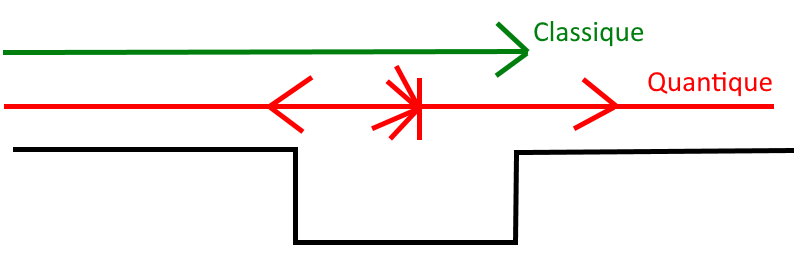
\includegraphics[scale=0.3]{6-1-puits-de-potentiel-ok.png}
\end{center}

$\blacktriangleright$ une particule incidente avec une petite énergie $E_k$ sur un mur ou une marche de potentiel. Quantiquement, la particule traverse par effet tunnel. Classiquement, la particule rebondit toujours.

\begin{center}
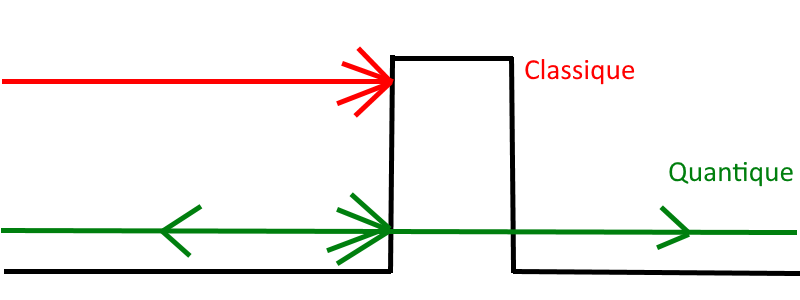
\includegraphics[scale=0.3]{6-1-effet-tunnel-ok.png}
\end{center}

$\blacktriangleright$ une particule arrivant sur un mur ou une marche de potentiel avec une énergie $E_k$ suffisamment grande, supérieure à l'énergie $E_p$ (à la \enquote{hauteur} de la marche ou du mur). Quantiquement, la particule peut rebondir. Classiquement, elle passe toujours.

\begin{center}
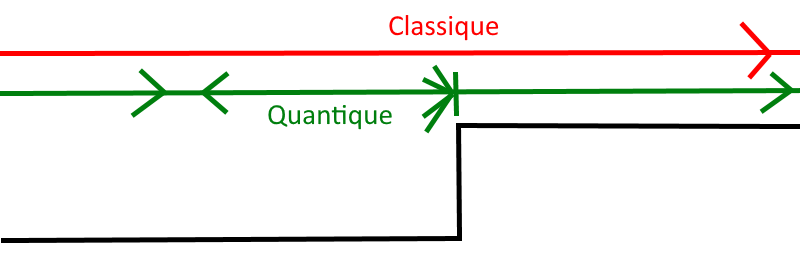
\includegraphics[scale=0.3]{6-1-marche-potentiel-ok.png}
\end{center}

\paragraph*{Remarque :}

Dans cette partie, on découvre le lien indissociable entre les conditions imposées à la fonction d'onde, solution de l'équation de Schrödinger et l'apparition spontanée de la quantification de l'énergie.

Trois cas sont à étudier : le mur, le puits et la barrière de potentiel.

\section{Propriété générale des problèmes à une dimension}

On s'intéresse uniquement aux états stationnaires, fonctions propres de $H$. Elles sont de la forme :
\begin{equation*}
\Psi (x,t) = exp \left( \frac{-i E t}{\hbar} \right) \Psi (x)
\end{equation*}
L'équation de Schrödinger se résume à l'équation aux valeurs propres. L'équation de Schrödinger : $H \ket\Psi = E \ket\Psi$.

On choisit la représentation $\lbrace \ket{x} \rbrace$, on projette l'équation vectorielle sur le bra $\bra{x}$ :
\begin{equation*}
\braket{x \vert H \vert \Psi} = \braket{x \vert E \vert \Psi}
\end{equation*}
Ce qui nous donne :
\begin{equation*}
\braket{x \vert \frac{p^2}{2m} + V(x) \vert \Psi} = E \braket{x \vert \Psi} = E \Psi (x)
\end{equation*}
Nous savons également que : $\braket{x \vert P \vert \Psi} = \frac{- \hbar^2}{i} \frac{\partial}{\partial x} \Psi (x) $

D'où :
\begin{align*}
\braket{x \vert \frac{p^2}{2m} \vert \Psi} &= \frac{- \hbar^2}{2 m} \frac{d^2}{dx^2} \Psi (x)\\
\braket{x \vert V(x) \vert \Psi} &= V(x) \Psi (x)
\end{align*}

L'équation de Schrödinger :
\begin{equation*}
\left[ \frac{- \hbar^2}{2m} \frac{d^2}{dx^2} + V(x) \right] \Psi (x) = E \Psi (x)
\end{equation*}
On fait un changement de variable :
\begin{center}
$V(x) = \frac{\hbar^2}{2m} U(x)$ et $E = \frac{\hbar^2}{2m} \mathcal{E}$
\end{center}

\underline{Étude dimensionnelle :}

\begin{align*}
[V] &= [E] = [M L^2 T^{-2}]\\
[h] &= \frac{[E]}{[\omega]} = [E] \times [T] = [M L^2 T^{-1}]\\
[U] &= \frac{[V][M]}{[\hbar]^2} = \frac{[M]}{[E][T][T]} = \frac{[M]}{[M L^2 T^{-2}][T]^2} = [L]^{-2}
\end{align*}
De même $[\mathcal{E}] = [L^{-2}]$

L'équation devient :
\begin{equation*}
-\frac{d^2}{dx^2} \Psi (x) + (\mathcal{E} - U(x)) \Psi(x) = 0
\end{equation*}
C'est une équation de Sturm-Liouville. Une équation linéaire homogène du second ordre. On ne s'intéresse qu'aux solution de carré sommable. Ces solutions sont des fonctions propres de $H$.

\subsection{La continuité de la fonction d'onde et de sa dérivée}

Quand $V(x)$ est continu, aucun problème ne se pose pour la continuité de $\Psi''(x)$. Analysons le cas où $V(x)$ présente un saut d'amplitude finie.\\

\begin{center}
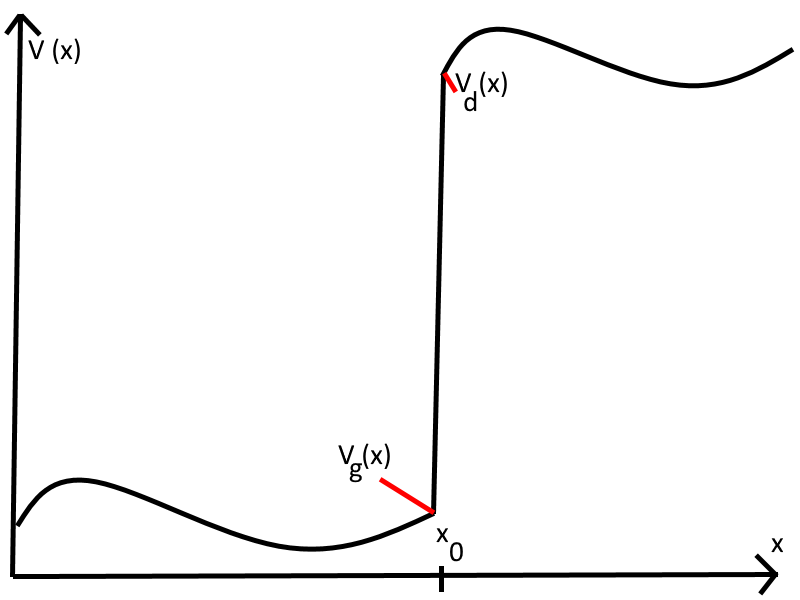
\includegraphics[scale=0.4]{6_2_1-V-x.png}
\end{center}

Pour étudier $\Psi (x)$ et sa dérivée, on intègre l'équation différentielle au voisinage de $x_0$.

\begin{equation*}
\Psi' (x_0 - \delta_x) - \Psi' (x_0 + \delta_x) = \int_{x_0 - \delta_x}^{x_0 + \delta_x} \left( U (x) - \mathcal{E} \right) \Psi (x) dx
\end{equation*}

À la limite quand $\delta_x$ tend vers 0, cela nous donne $\Psi' (x_0 - \delta_x) - \Psi' (x_0 + \delta_x) = 0$. $\Psi' (x)$ est continue au point $x_0$ où le potentiel effectue un saut d'amplitude finie. La continuité de $\Psi' (x)$ entraîne la continuité de $\Psi (x)$. $\Psi'' (x)$ est discontinue, cette propriété apparaît dans l'équation différentielle.

\begin{align*}
\Psi_{I}'' (x_0) + ( \mathcal{E} - V_g (x_0) ) \Psi_{I} (x_0) &= 0\\
\Psi_{II}'' (x_0) + ( \mathcal{E} - V_d (x_0) ) \Psi_{II} (x_0) &= 0\\
\Psi_{II}'' (x_0) - \Psi_{II} (x_0) &= ( V_d (x_0) - V_g (x_0) ) \Psi (x_0)
\end{align*}
Car : $\Psi_{I} (x_0) = \Psi_{II} (x_0)$

Classiquement, la discontinuité de $\Psi''$ est comprise comme étant une variation instantanée de l'énergie $E_k$.

\begin{equation*}
\frac{p^2}{2m} \Psi (x) = \frac{\Psi'' \hbar^2}{2m} = \braket{x \vert \frac{p^2}{2m} \vert \Psi}
\end{equation*}

Sachant que $E = E_k + V(x)$ ; l'énergie mécanique est égale à la valeur propre de $H$, elle est constante, toute variation brusque de $V(x)$ entraîne la variation de l'énergie $E_k$, à la hausse comme à la baisse.

\paragraph*{Remarque :} Nous traiterons à part, en Travaux Dirigés, le cas où $V(x)$ effectue un saut infinie : le puits de potentiel infinie et le cas où $V(x) = \delta (x)$. 

\subsection{Le théorème de Wronshien}

Soit deux fonctions solutions de l'équation de Schrödinger $\Psi_1 (x)$ et $\Psi_2 (x)$ associées à deux valeurs $E_1$ et $E_2$.
\begin{center}
\textbf{a)} $\Psi_1 '' (x) + (E_1 - U(x)) \Psi_1 (x) = 0 \cdot \Psi_2 (x)$\\

\textbf{b)} $\Psi_2 '' (x) + (E_2 - U(x)) \Psi_2 (x) = 0 \cdot \Psi_1 (x)$
\end{center}

Le Wronshien est définit comme suit : 
\begin{center}
\[
W [\Psi_1 (x) , \Psi_2 (x)] = \Psi_1 (x) \Psi_2 ' (x) - \Psi_1 ' (x) \Psi_2 (x) \longrightarrow
\left\lbrace
\begin{matrix}
\Psi_1 (x) & \Psi_2 (x)\\
\Psi_1 ' (x) & \Psi_2 ' (x)
\end{matrix}
\right\rbrace
\]
\end{center}
On calcule $(a) - (b)$.
\begin{equation*}
\Psi_1 '' (x) \Psi_2  (x) - \Psi_2 '' (x) \Psi_1 (x) = (E_1 - E_2) \Psi_1 (x) \Psi_2 (x)
\end{equation*}
On ajoute et on retranche $\Psi_1 ' (x) \Psi_2 ' (x)$ et on intègre l'égalité entre \textbf{a)} et \textbf{b)} ; on trouve :
\begin{equation*}
\left[ \Psi_1 (x) \Psi_2 ' (x) - \Psi_1 ' (x) \Psi_2 (x) \right]_a^b = (E_1 - E_2) \int_a^b \Psi_1 (x) \Psi_2 (x) dx
\end{equation*}
Cette relation constitue la formulation simplifiée du théorème de Wronshien.

\subsection{Tout état lié à une dimension est non dégénérée}

Considérons le cas où : $E_1 = E_2$. On obtient : $\left[ \Psi_1 ' (x) \Psi_2 (x) - \Psi_1 \Psi_2 ' (x) \right]_a^b = 0$. Comme $a$ et $b$ sont des points arbitraires, on peut affirmer que le \enquote{Wronshien} de deux solutions indépendantes associées à une même valeur propre est constante. Or, un état lié est forcément nul à infinie, enfin sa fonction d'onde... . D'où le Wronshien à sa définition est forcément nul à infinie et prend la même valeur partout pour tout $x$. $W[\Psi_1 (x) \Psi_2 (x)]=0$ d'où $\Psi_1 ' (x) \Psi_2 (x) = \Psi_1 (x) \Psi_2 ' (x)$. La résolution de cette équation est simple :
\begin{center}
$Ln \Psi_1 (x) = Ln \Psi_2 (x) + k$ et $\Psi_1 (x) = \alpha \Psi_2 (x)$
\end{center}
D'où la propriété : a une dimension, tout état lié est non-dégénéré !

\subsection{Les états liés sont deux à deux orthogonaux entre eux}

En effet, en choisissant pour $a$ et $b$ les limites du domaines du confinement. Le Wronshien est nul, l'intégrale entre $a$ et $b$ de $\Psi_1 (x)$ et $\Psi_2 (x) dx = 0$ ; donc $\Psi_1 (x) \perp \Psi_2 (x)$.

\begin{center}
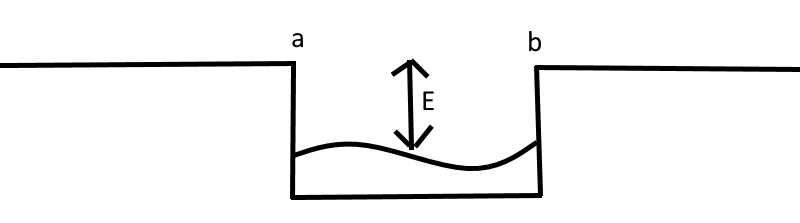
\includegraphics[scale=0.4]{6-2-4-Confinement.png}
\end{center}

\subsection{Toute valeur propre de $H$ ne peut être inférieure au minimum de V(x)}

Supposons que $V(x)$ est borné inférieur uniformément et son minimum est $V_{min}$ (ici nous considérons un puits de potentiel fini) et on s'intéresse aux états liés. On suppose que $E < V_{min}$, dans cette solution, l'équation de Schrödinger est :
\begin{center}
$\Psi'' = \underbrace{-E + V(x)}_{> 0} \Psi$ ; $-E + V(x) > 0$ et $V(x) > 0$
\end{center}
Donc $\Psi''$ et $\Psi$ sont de même signe.

\begin{center}
\includegraphics[scale=0.4]{6_2_5-figure1.png}
\end{center}

Or les fonctions représentées par ces courbes ne sont pas de carré sommable, ce qui est absurde, donc $E > V(x)$. Pour le puits de potentiel fini :

\begin{center}
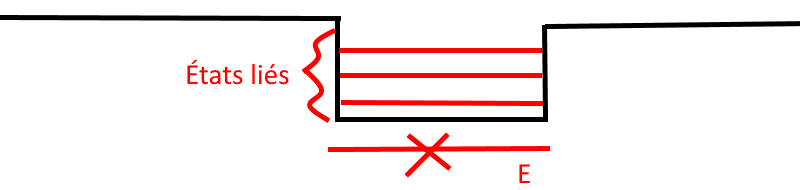
\includegraphics[scale=0.4]{6-2-5-figure2-ok.png}
\end{center}

\section{Cas des puits symétriques V(x) = V(-x)}

Rappel sur l'opérateur parité $\Pi$. Son action sur une fonction d'onde $\Pi \Psi (x) = \Psi (-x)$ avec $\Pi^2 = I$ et les valeurs propres de $\Pi$ sont $\lambda = \pm 1$. Les fonctions associées à $\lambda = 1$ sont les fonctions paires : $\Pi \Psi (x) = \Psi (-x) = \Psi (x)$. Les fonctions associées à $\lambda = -1$ sont les fonctions impaires : $\Pi \Psi (x) = \Psi (-x) = -\Psi (x)$. Montrons que $\Pi$ commute avec $p^2 = -\hbar^2 \frac{\partial^2}{\partial x^2}$.
\begin{equation*}
\frac{\hbar}{i} \frac{\partial}{\partial x} \left( \Pi \Psi (x) \right) = \frac{\hbar}{i} \frac{\partial}{\partial x} \Psi (-x) = \frac{\hbar}{i} \Psi' (-x)
\end{equation*}
On arrive à : $\left[ \Pi \frac{\hbar}{i} \frac{\partial}{\partial x} \right] = 0$.

Testons les commutations entre $\Pi$ et $p^2$ :
\begin{align*}
- \hbar^2 \frac{\partial^2}{\partial x^2} \Pi \Psi (x) &= \frac{\hbar}{\partial x^2} \Psi (-x) = -\hbar^2 \Psi'' (-x)\\
\Pi \left( -\hbar^2 \frac{\partial}{\partial x} \Psi (x) \right) &= -\hbar \Psi'' (-x)
\end{align*}
Donc $[\Pi ; p^2] = 0$.\\

Analysons la commutation de $\Pi$ avec $V(x)$, calcul de $\Pi V(x) \Psi (x) = V(-x) \Psi (-x) = V(x) \Psi (-x)$ ; $V(x)$ est une fonction paire. Calculons $V(x) \Pi \Psi (x) = V(x) \Psi (-x)$, d'où $[V(x) , \Pi] = 0$ et $[H , \Pi] = 0$. $\Pi$ commute avec $H$, d'où ils possèdent des fonctions propres communes. Les fonctions propres de $H$ sont aussi des fonctions propres de $\Pi$ donc elles ont aussi une parité définie : elles sont des fonctions paires ou impaires.

\chapter{L'OSCILLATEUR HARMONIQUE}

Ce chapitre porte sur la bête noire de tout apprenti physicien : l'oscillateur harmonique. Mais ici, dans le cadre de la mécanique quantique !

\newpage
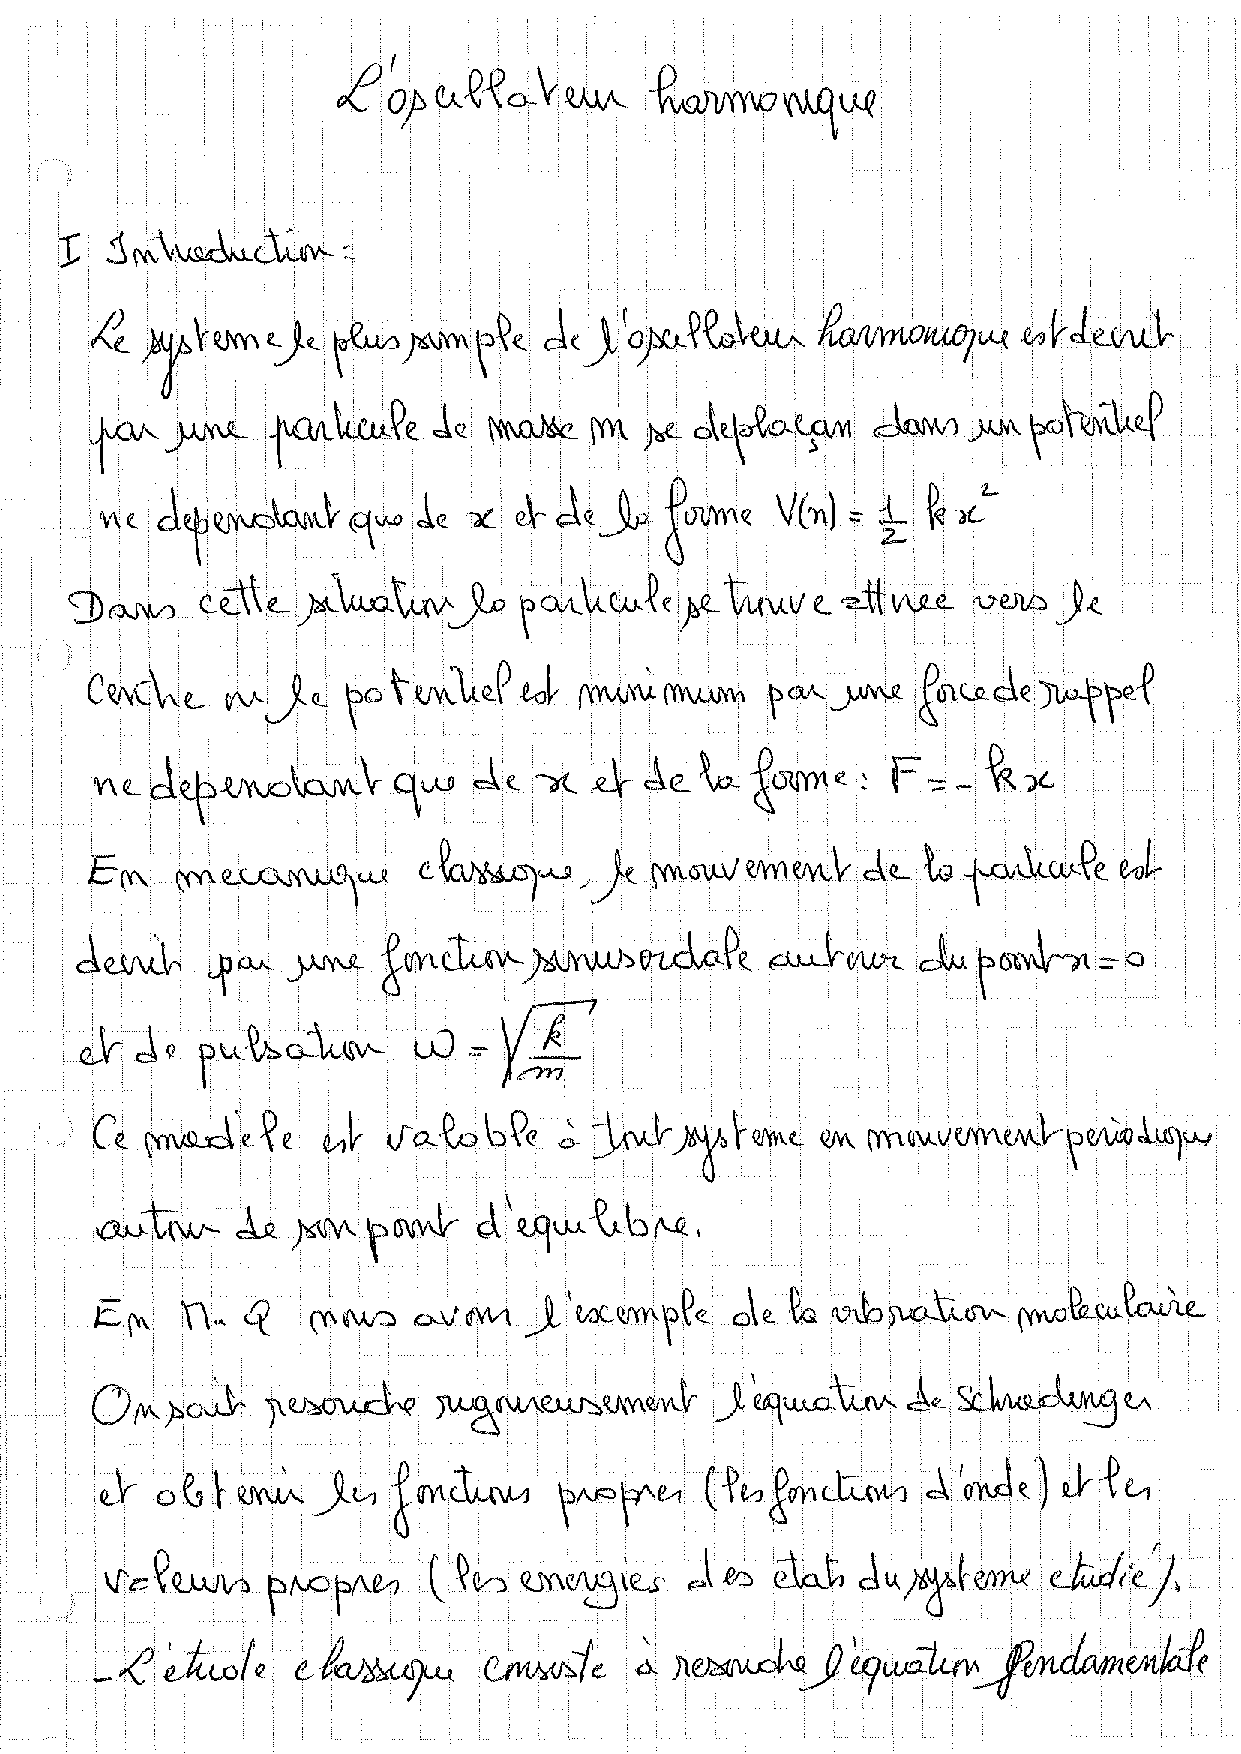
\includepdf[scale=0.95,pages=1-7]{cours-oscillateur-part1.pdf}
\newpage
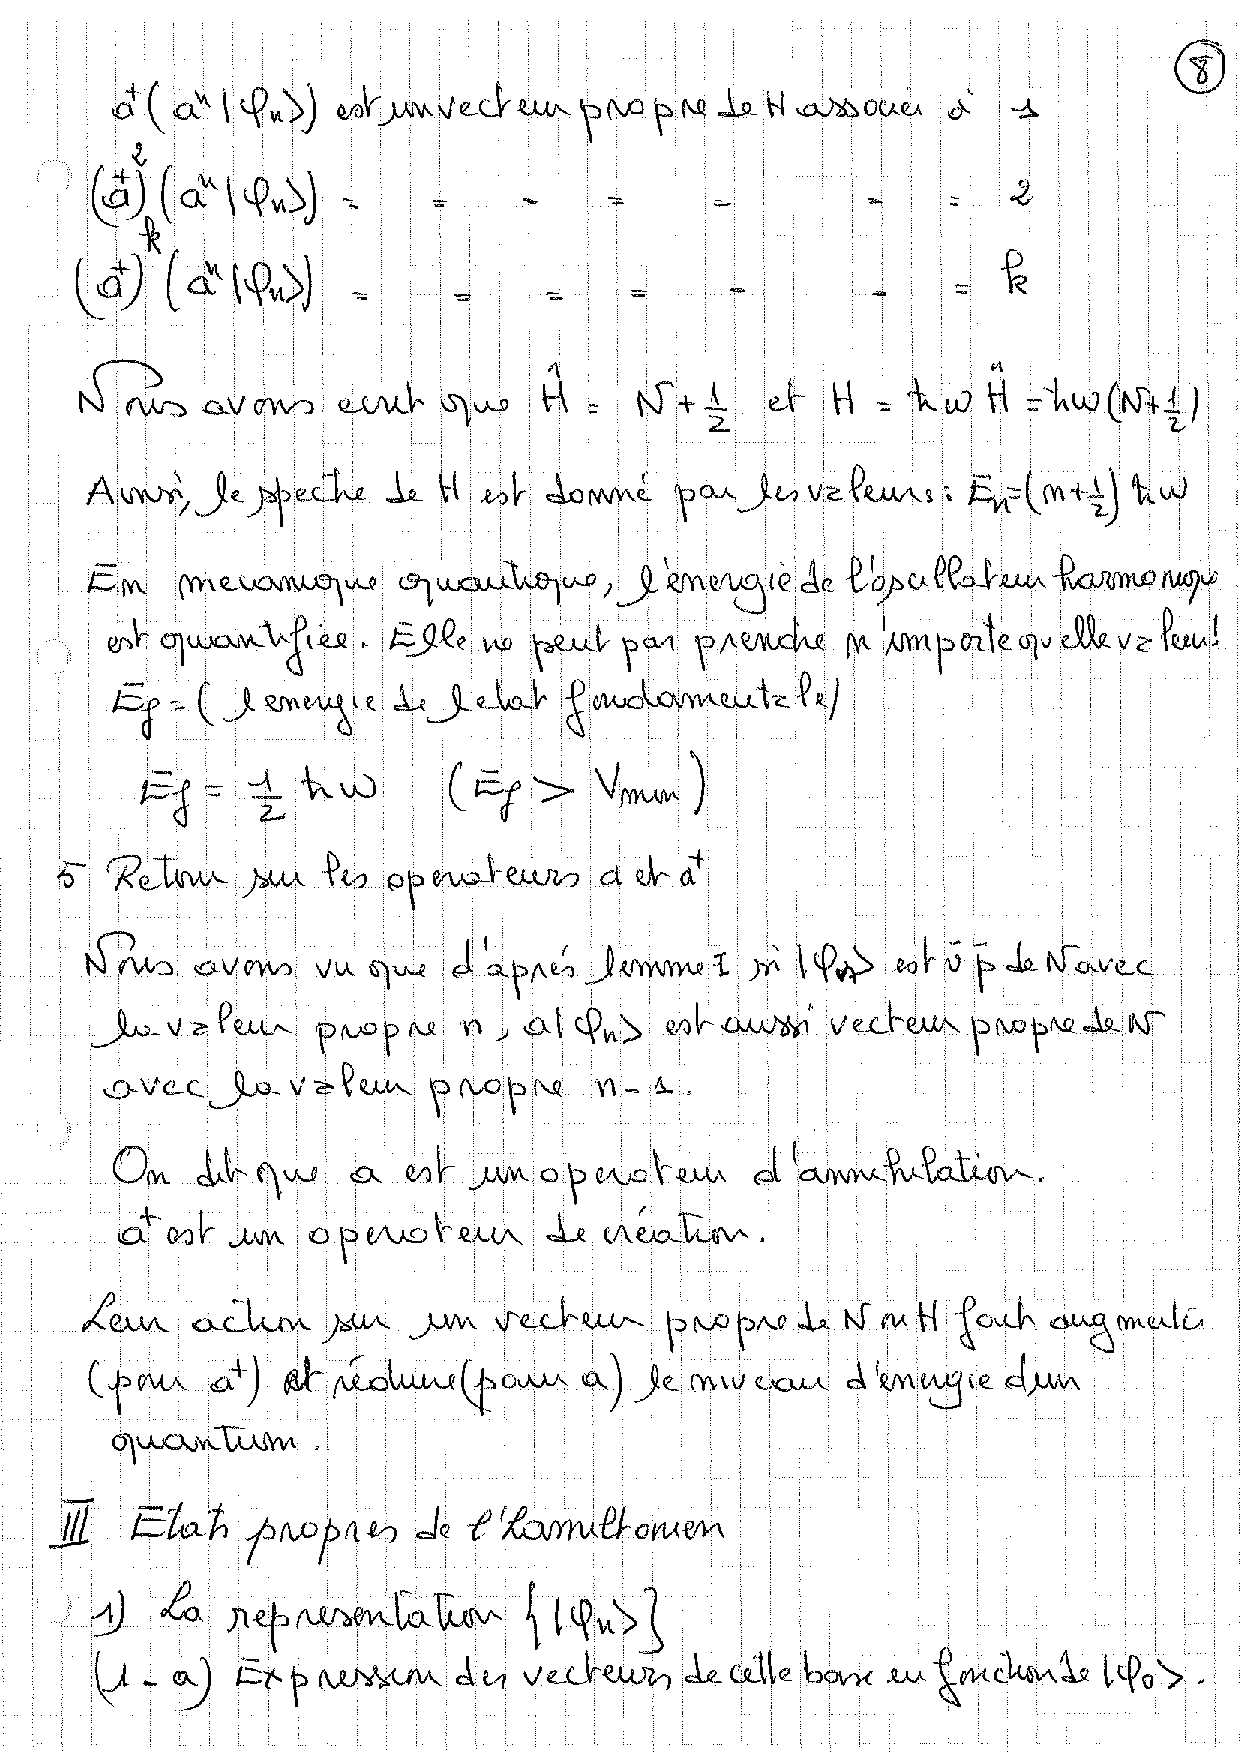
\includepdf[scale=0.95,pages=1-8]{cours-oscillateur-part2.pdf}

\chapter{LES ÉTATS NON LIÉS}

\newpage
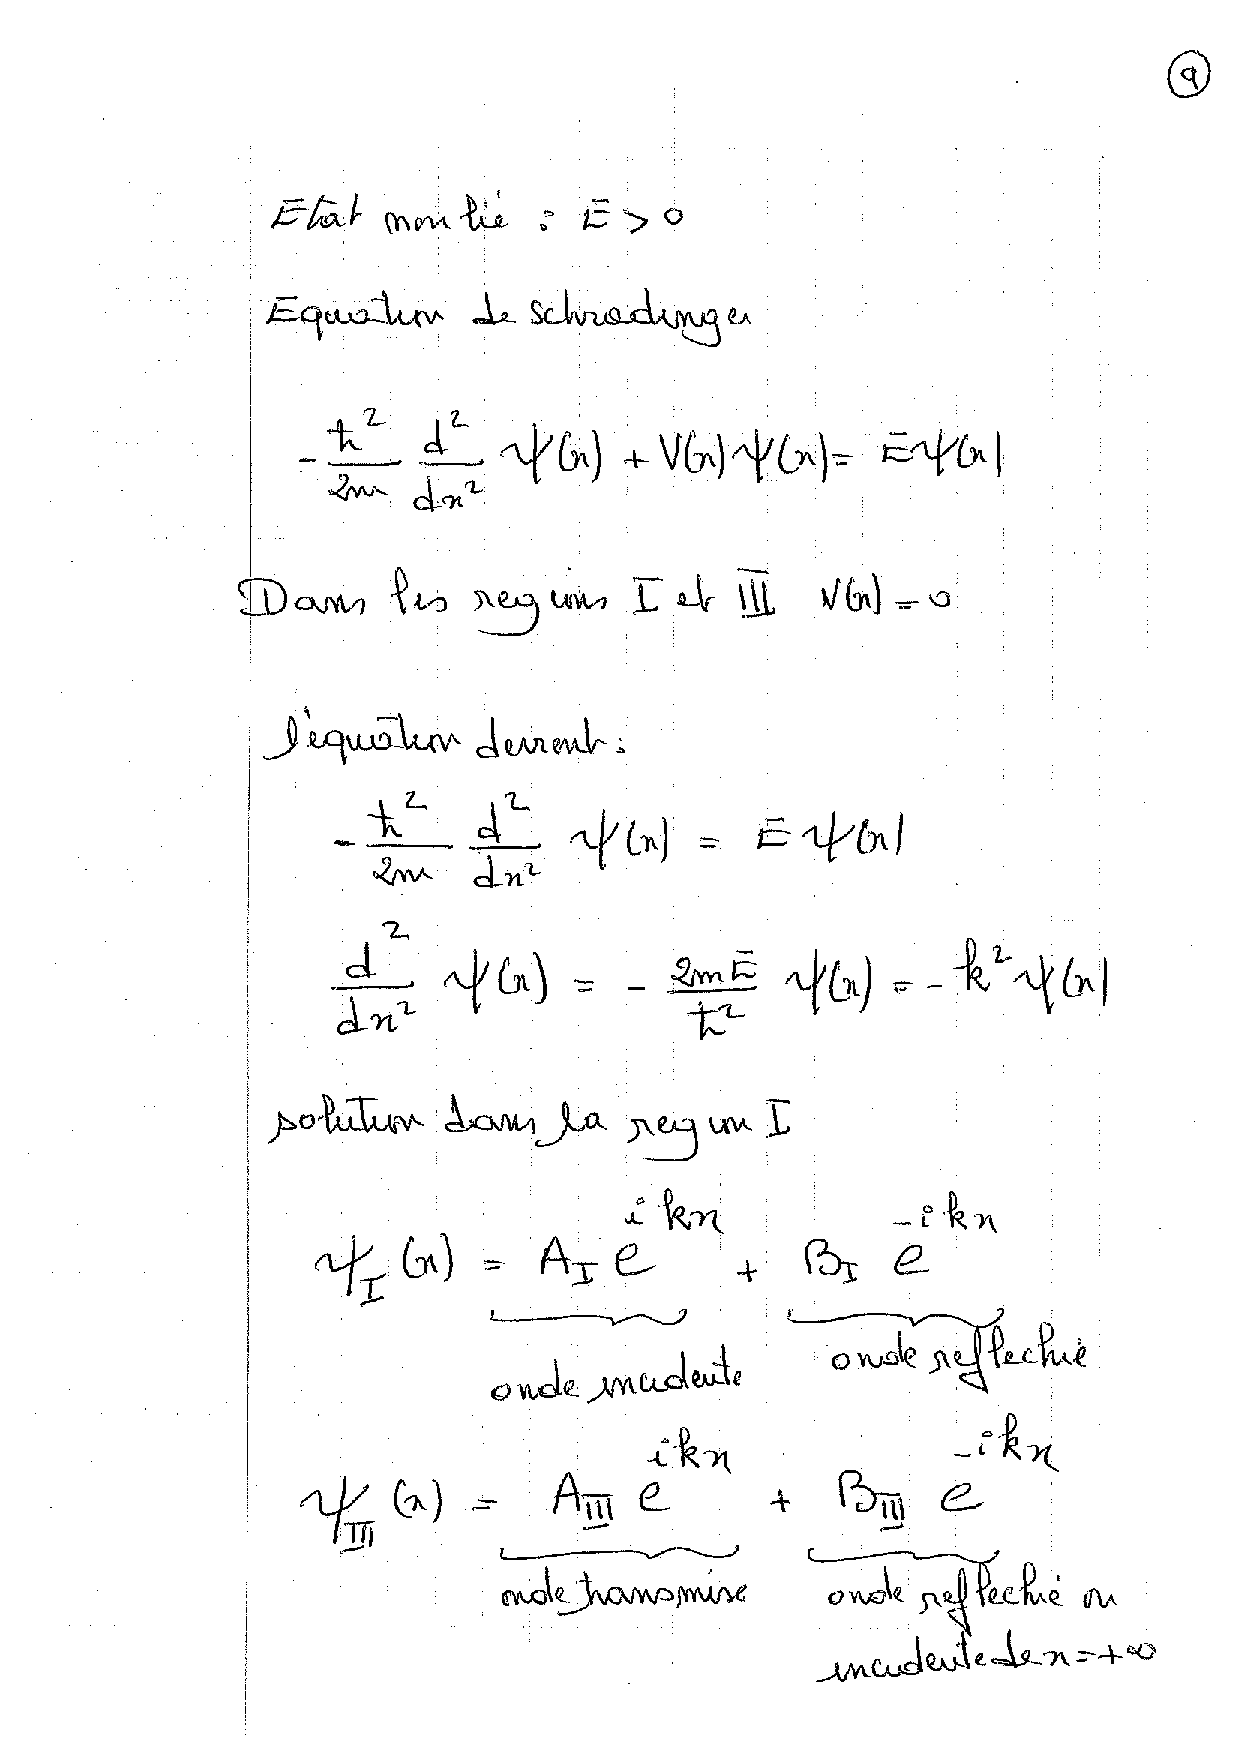
\includepdf[scale=0.95,pages=1-7]{Etat-non-lie.pdf}

\chapter{LE MOMENT CINÉTIQUE}

\newpage
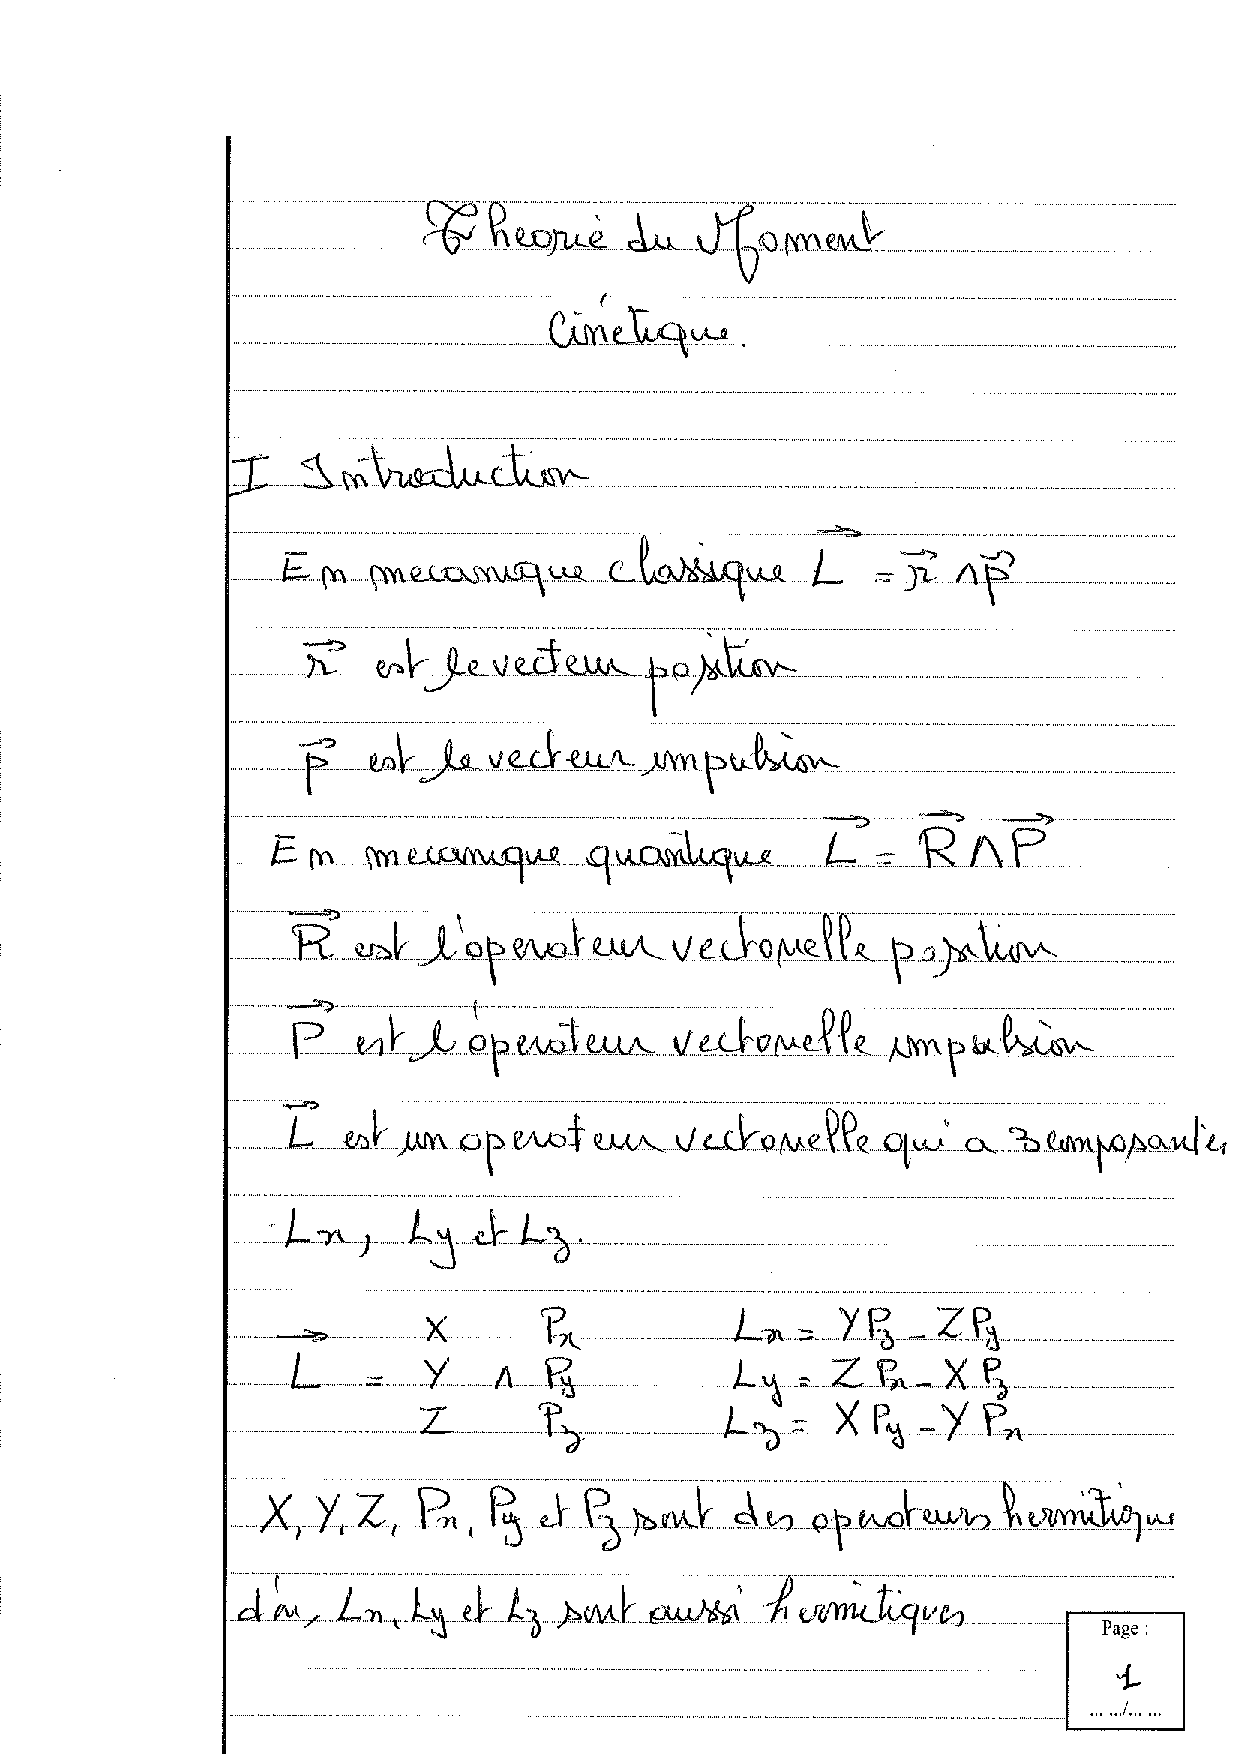
\includepdf[scale=0.95,pages=1-8]{momentcinetique-1.pdf}
\newpage
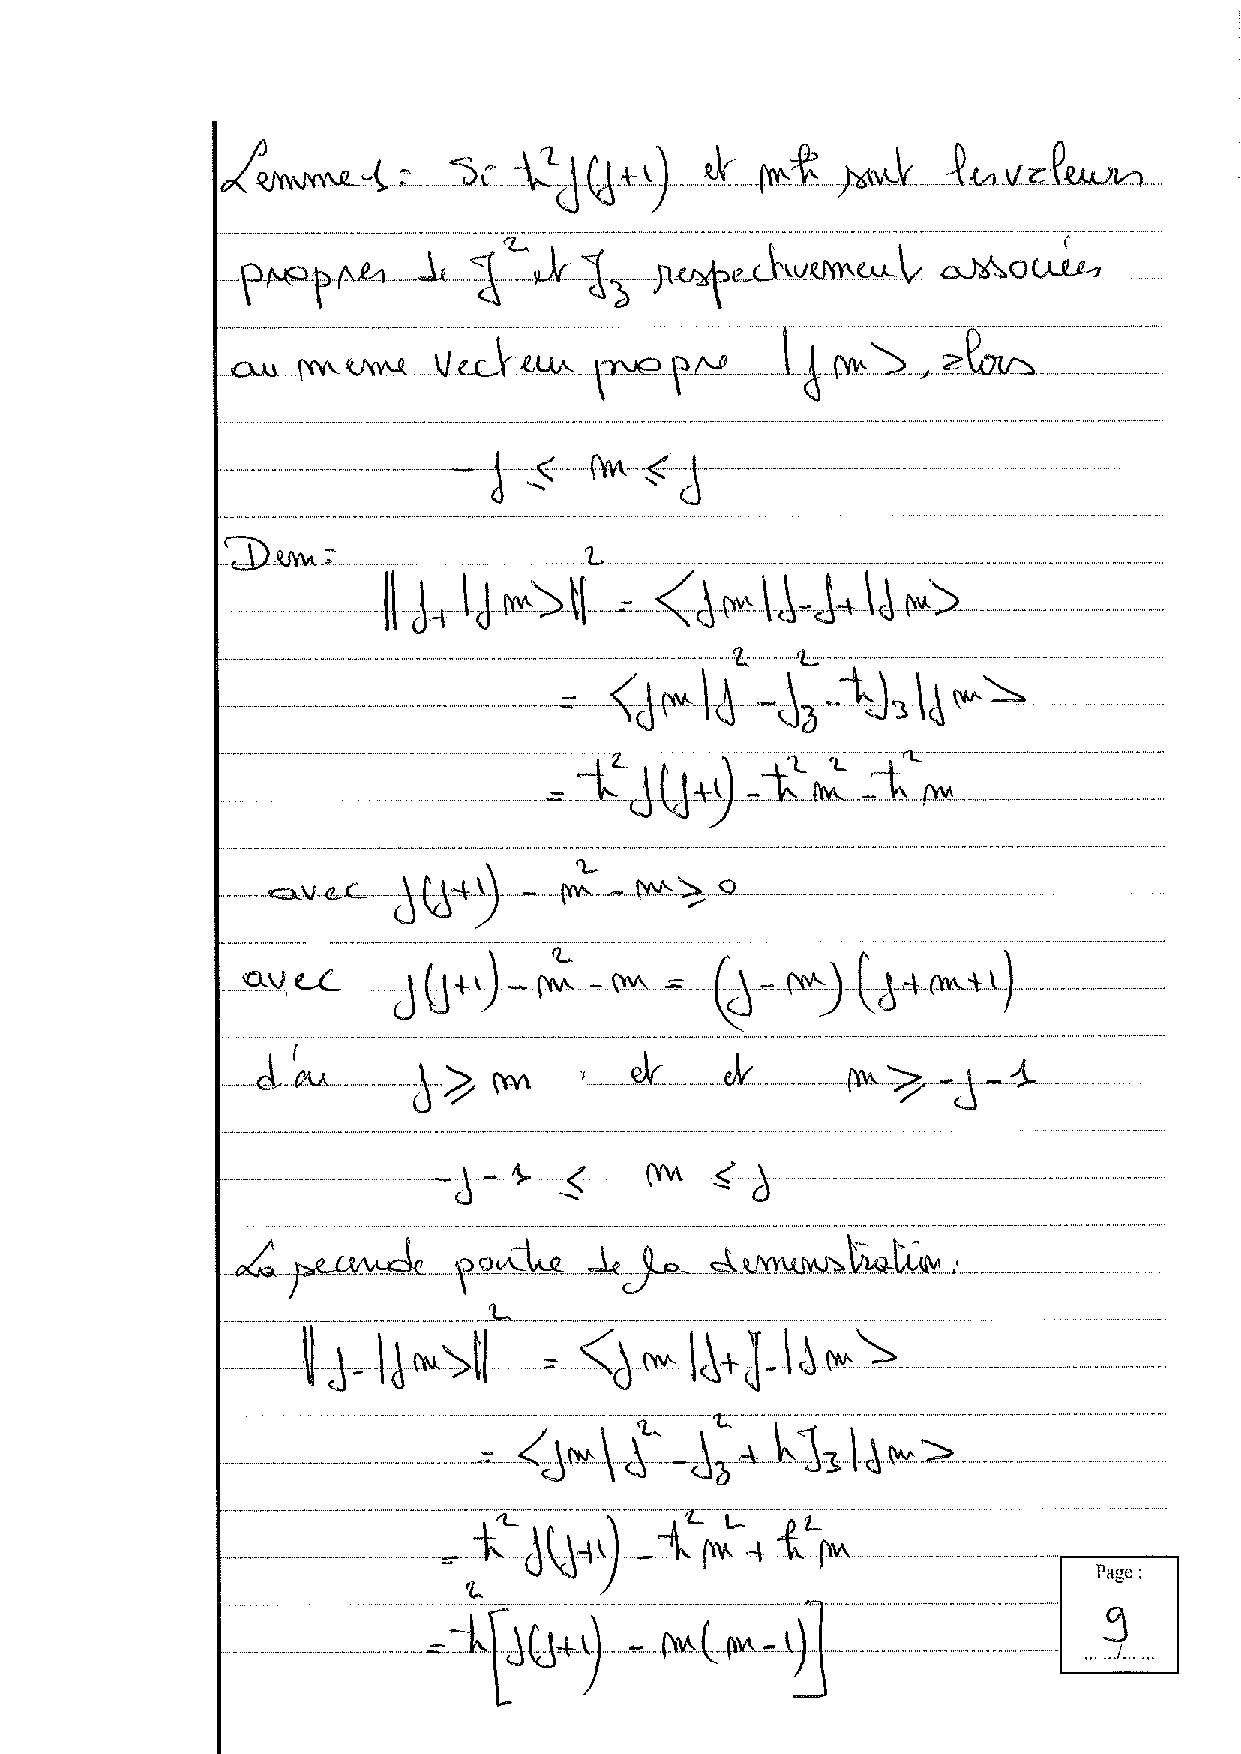
\includepdf[scale=0.95,pages=1-7]{momentcinetique-2.pdf}
\newpage
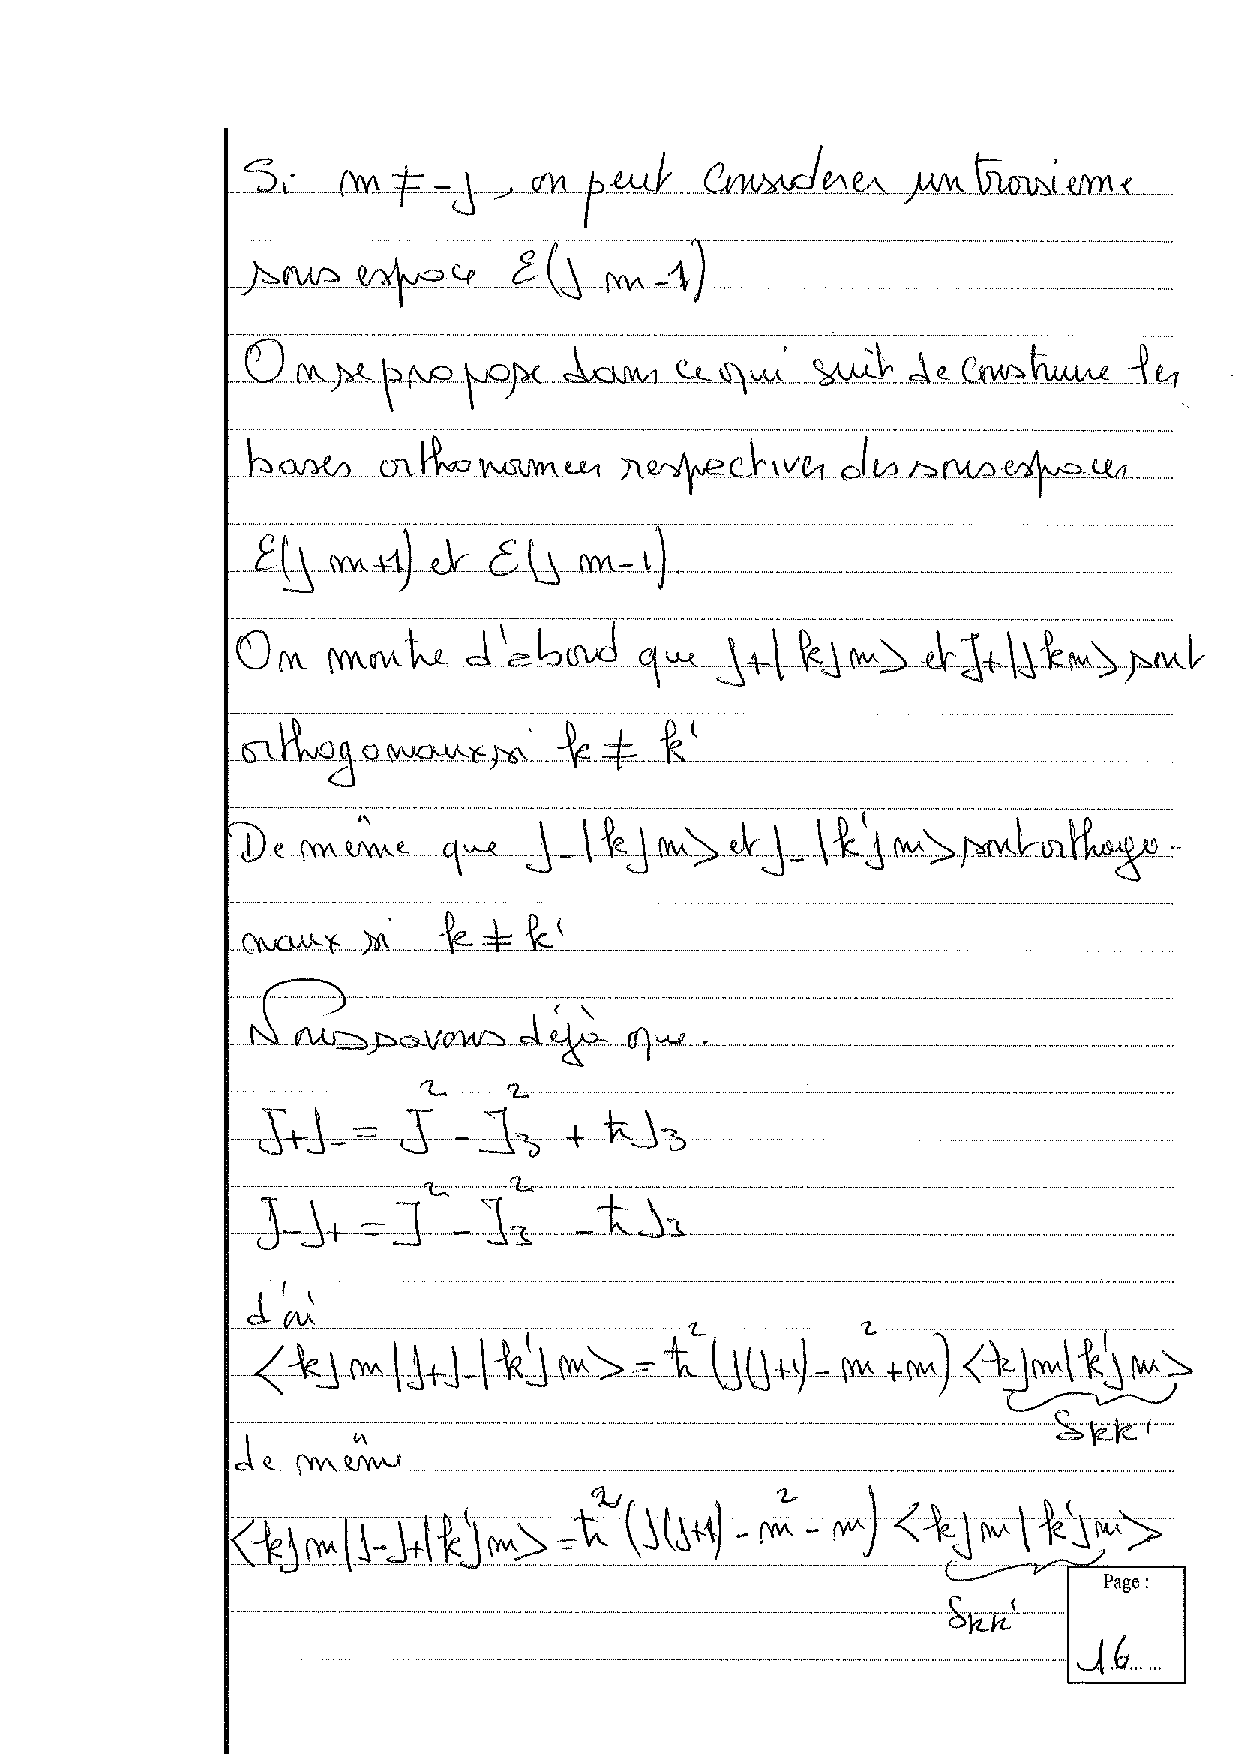
\includepdf[scale=0.95,pages=1-9]{momentcinetique-3.pdf}

\chapter{LA THÉORIE DES PERTURBATIONS}

Ce chapitre consiste en une résolution de l'exercice, dont l'énoncé se trouve à la page suivante. Cette résolution a été fourni par le professeur via \enquote{Moodle} en format pdf.

\newpage
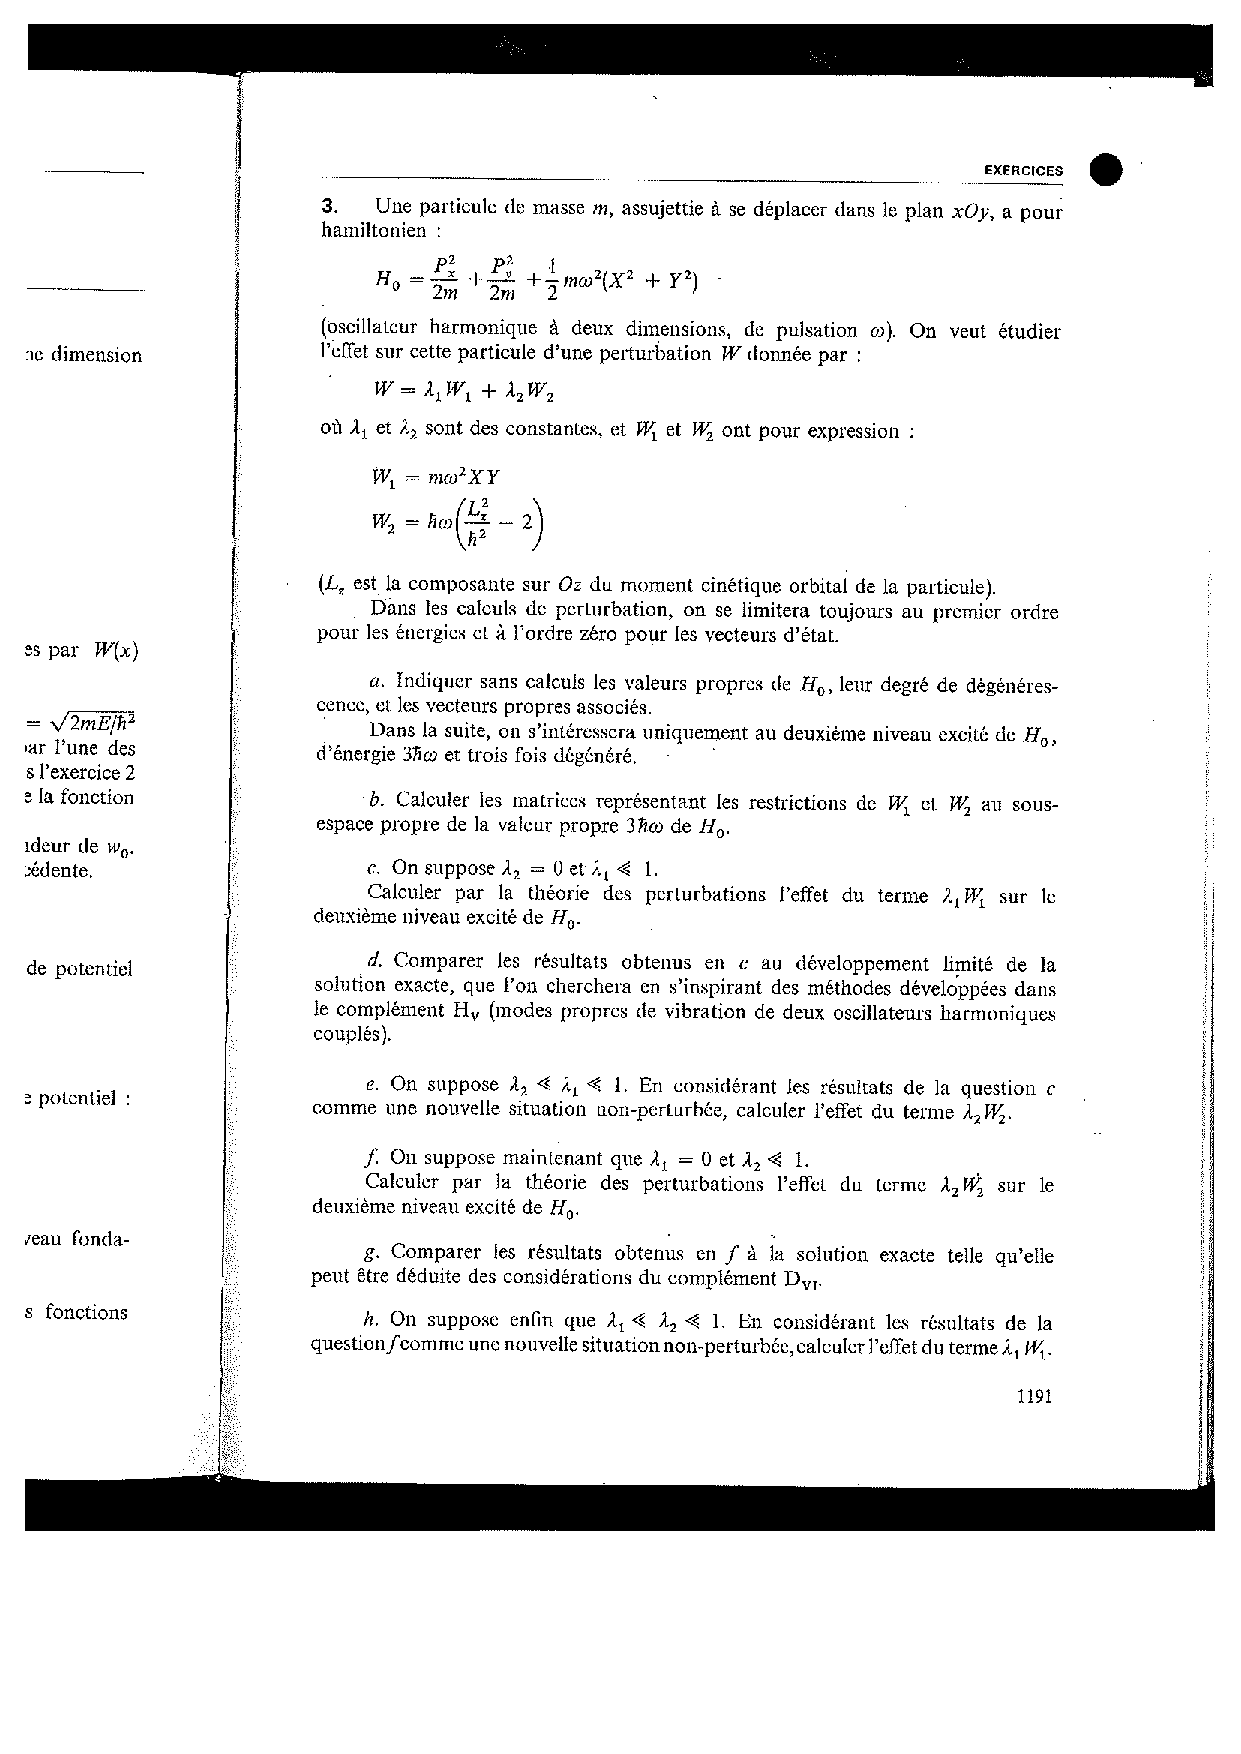
\includepdf[scale=0.95,pages=1-19]{theorie des Perturbations.pdf}

\chapter{L'ESSENTIEL DU COURS}

\section{Outils Mathématiques 1}

\section{Les postulats}

\section{Le magnétisme atomique}

\section{Outils Mathématiques 2}

\section{Produit tensoriel}

\section{Potentiel à une dimension constant par morceau}

\section{L'oscillateur harmonique}

\section{Les états non liés}

\section{Le moment cinétique}

\end{document}